% ****** Start of file apssamp.tex ******
%
%   This file is part of the APS files in the REVTeX 4.2 distribution.
%   Version 4.2a of REVTeX, December 2014
%
%   Copyright (c) 2014 The American Physical Society.
%
%   See the REVTeX 4 README file for restrictions and more information.
%
% TeX'ing this file requires that you have AMS-LaTeX 2.0 installed
% as well as the rest of the prerequisites for REVTeX 4.2
%
% See the REVTeX 4 README file
% It also requires running BibTeX. The commands are as follows:
%
%  1)  latex apssamp.tex
%  2)  bibtex apssamp
%  3)  latex apssamp.tex
%  4)  latex apssamp.tex
%
\maxdeadcycles=1000

\documentclass[%
 reprint,
%superscriptaddress,
%groupedaddress,
%unsortedaddress,
%runinaddress,
%frontmatterverbose, 
%preprint,
%preprintnumbers,
%nofootinbib,
%nobibnotes,
%bibnotes,
 amsmath,amssymb,
 aps,
 prd,
%prb,
%rmp,
%prstab,
%prstper,
floatfix,
twocolumn,
%linenumbers
]{revtex4-1}

\usepackage{graphicx}% Include figure files
\usepackage{dcolumn}% Align table columns on decimal point
\usepackage{bm}% bold math
\usepackage{multirow}
\usepackage{subfigure}

\usepackage{hyperref}
\hypersetup{
    bookmarks=true,
    colorlinks=true,
    citecolor=blue,
    filecolor=black,
    linkcolor=blue,
    linktoc=page,
    urlcolor=blue
}

\begin{document}

\preprint{APS/123-QED}

\title{Searth for right-handed neutrino with solar neutrino experiment}% 

\author{Yutao Zhu}
\author{Shaomin Chen}
\author{Zhicai Zhang}%
 \email{zhicaizhang@tsinghua.edu.cn}
\affiliation{%
 Department of Engineering Physics, Tsinghua University, Beijing 100084, China
}%

\date{\today}

\begin{abstract}
A searth for right-handed neutrino with solar neutrino experiment is presented.
\end{abstract}

\maketitle

\section{\label{sec:intro}  Introduction }
\section{\label{sec:productionAndDecay} Production and decay of right-handed neutrino }


\begin{figure}[!htbp]
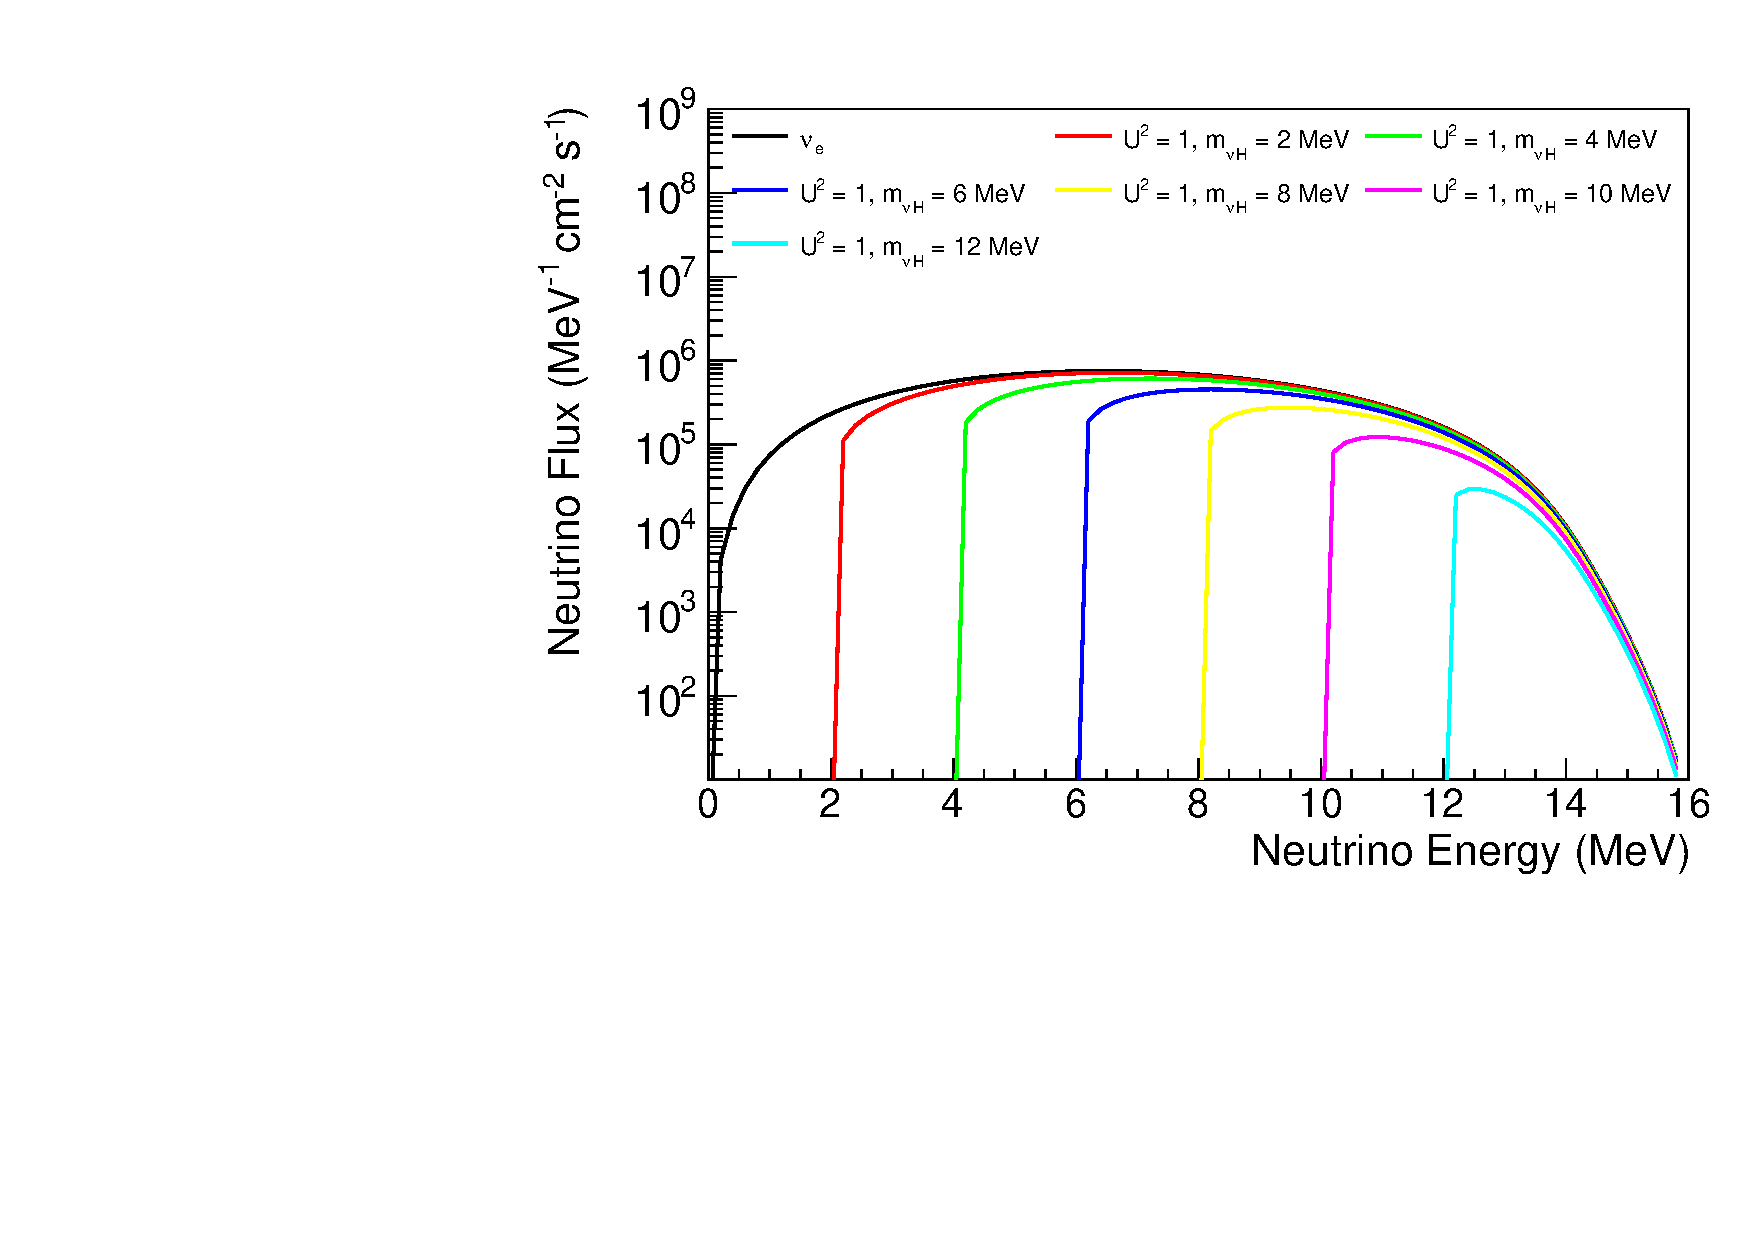
\includegraphics[width=0.99\columnwidth]{../plots/RHNSpectrum_U1.0_AllMass_linXlogY.pdf}
\caption{Energy spectra of right-handed neutrinos with different masses emitted from $^8$B decay in the Sun. The right-handed neutrino spectra are based on $^8B$ left-handed solar neutrino spectrum ($\nu_e$ in the plot, taken from~\cite{bahcall1996B8Spectrum}) and are suppressed by the mixing parameter $|U_{eH}|^2$ by $\Phi(E_{\nu H}) = |U_{eH}|^2\sqrt{1-(\frac{m_{\nu H}}{E_{\nu H}})^2}\Phi_{^8B}(E_{\nu})$, where $|U_{eH}|^2$ is 1.0 in this plot.}
\label{fig:RHNSpectrum} 
\end{figure}
%nuL numerical source: https://www.sns.ias.edu/~jnb/SNdata/Export/B8spectrum/b8spectrum.txt

\begin{figure}[!htbp]
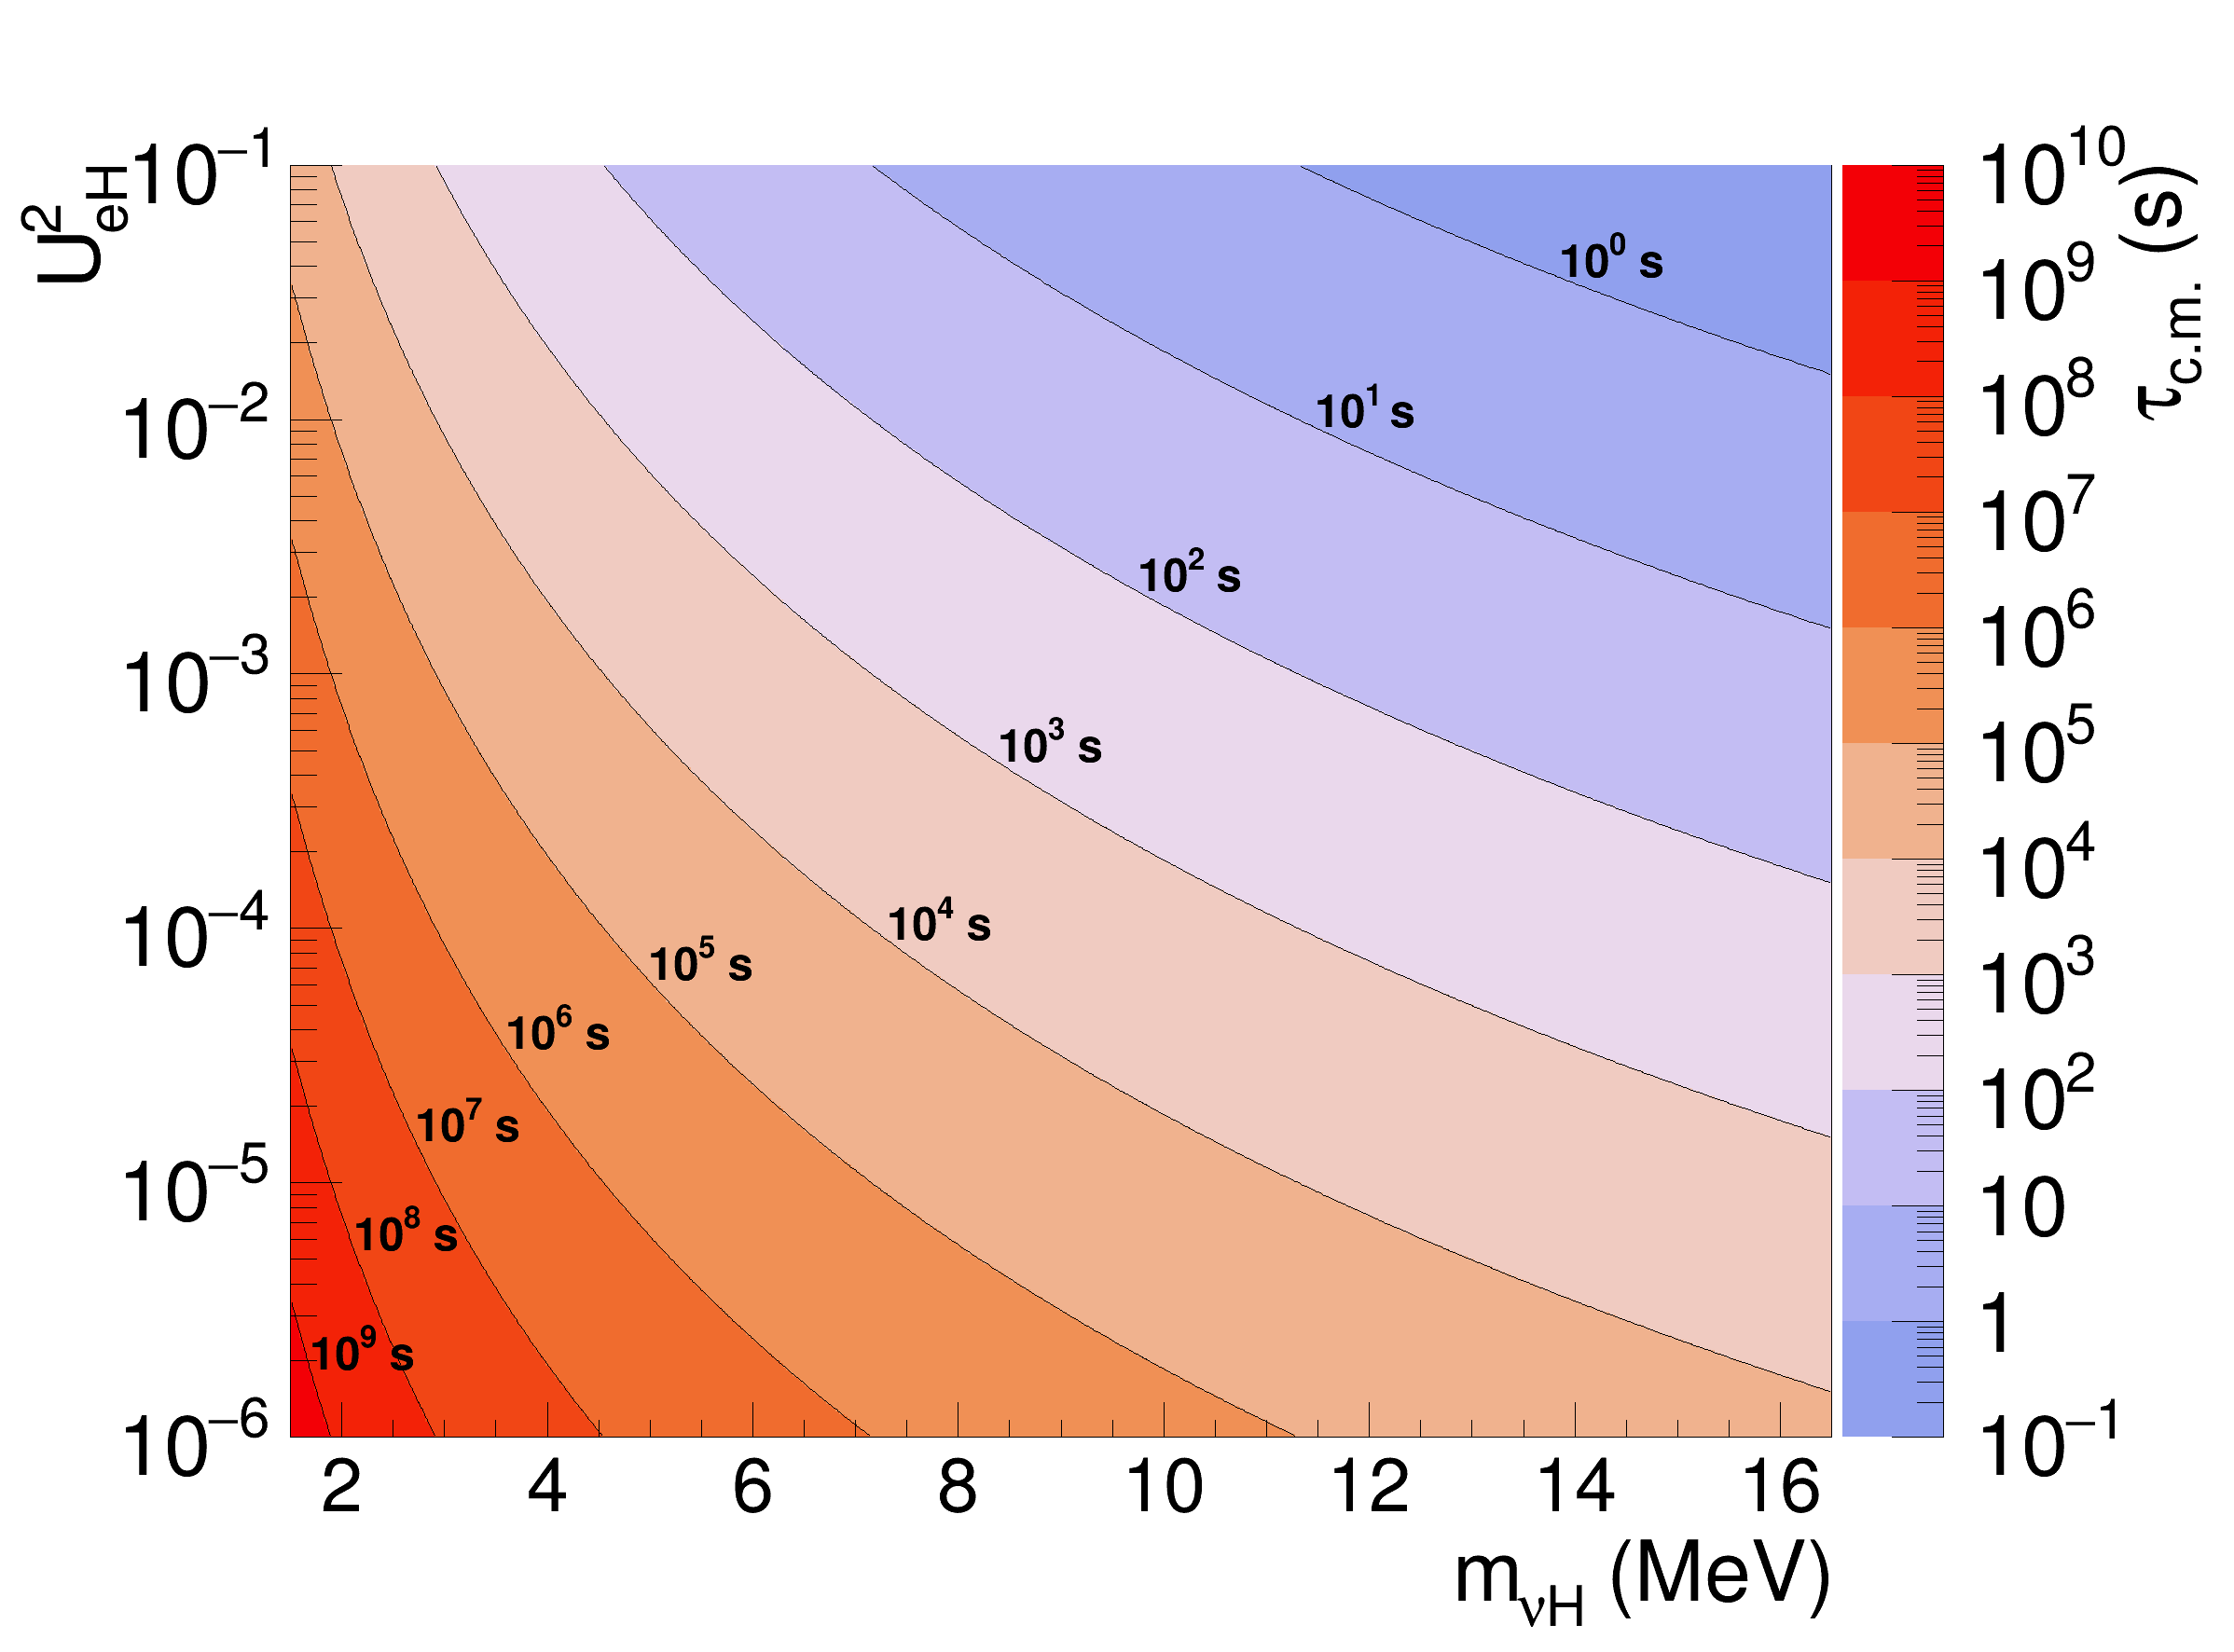
\includegraphics[width=0.99\columnwidth]{../plots/RHNTauCM_vs_M_U2_contour_linXlogYlogZ.png}
\caption{Proper lifetime ($\tau_{c.m}=1.0/\Gamma_{c.m.}^{tot}$) of right-handed neutrinos with different masses and different mixing parameter $|U_{eH}|^2$. The total width $\Gamma_{c.m.}^{tot}$ includes decays by both $W$ and $Z$ bosons, and is defined by $\Gamma_{c.m.}^{tot} = \frac{G_F^2}{192\pi^3}m_{\nu H}^5 |U_{eH}|^2 (1 + h\left[\frac{m_e^2}{m_{\nu H}^2}\right])$, where $h\left[\frac{m_e^2}{m_{\nu H}^2}\right])$ is the phase-space taken from~\cite{gorbunov2007TauCM}.}
\label{fig:RHNCTau} 
\end{figure}

\begin{figure}[!htbp]
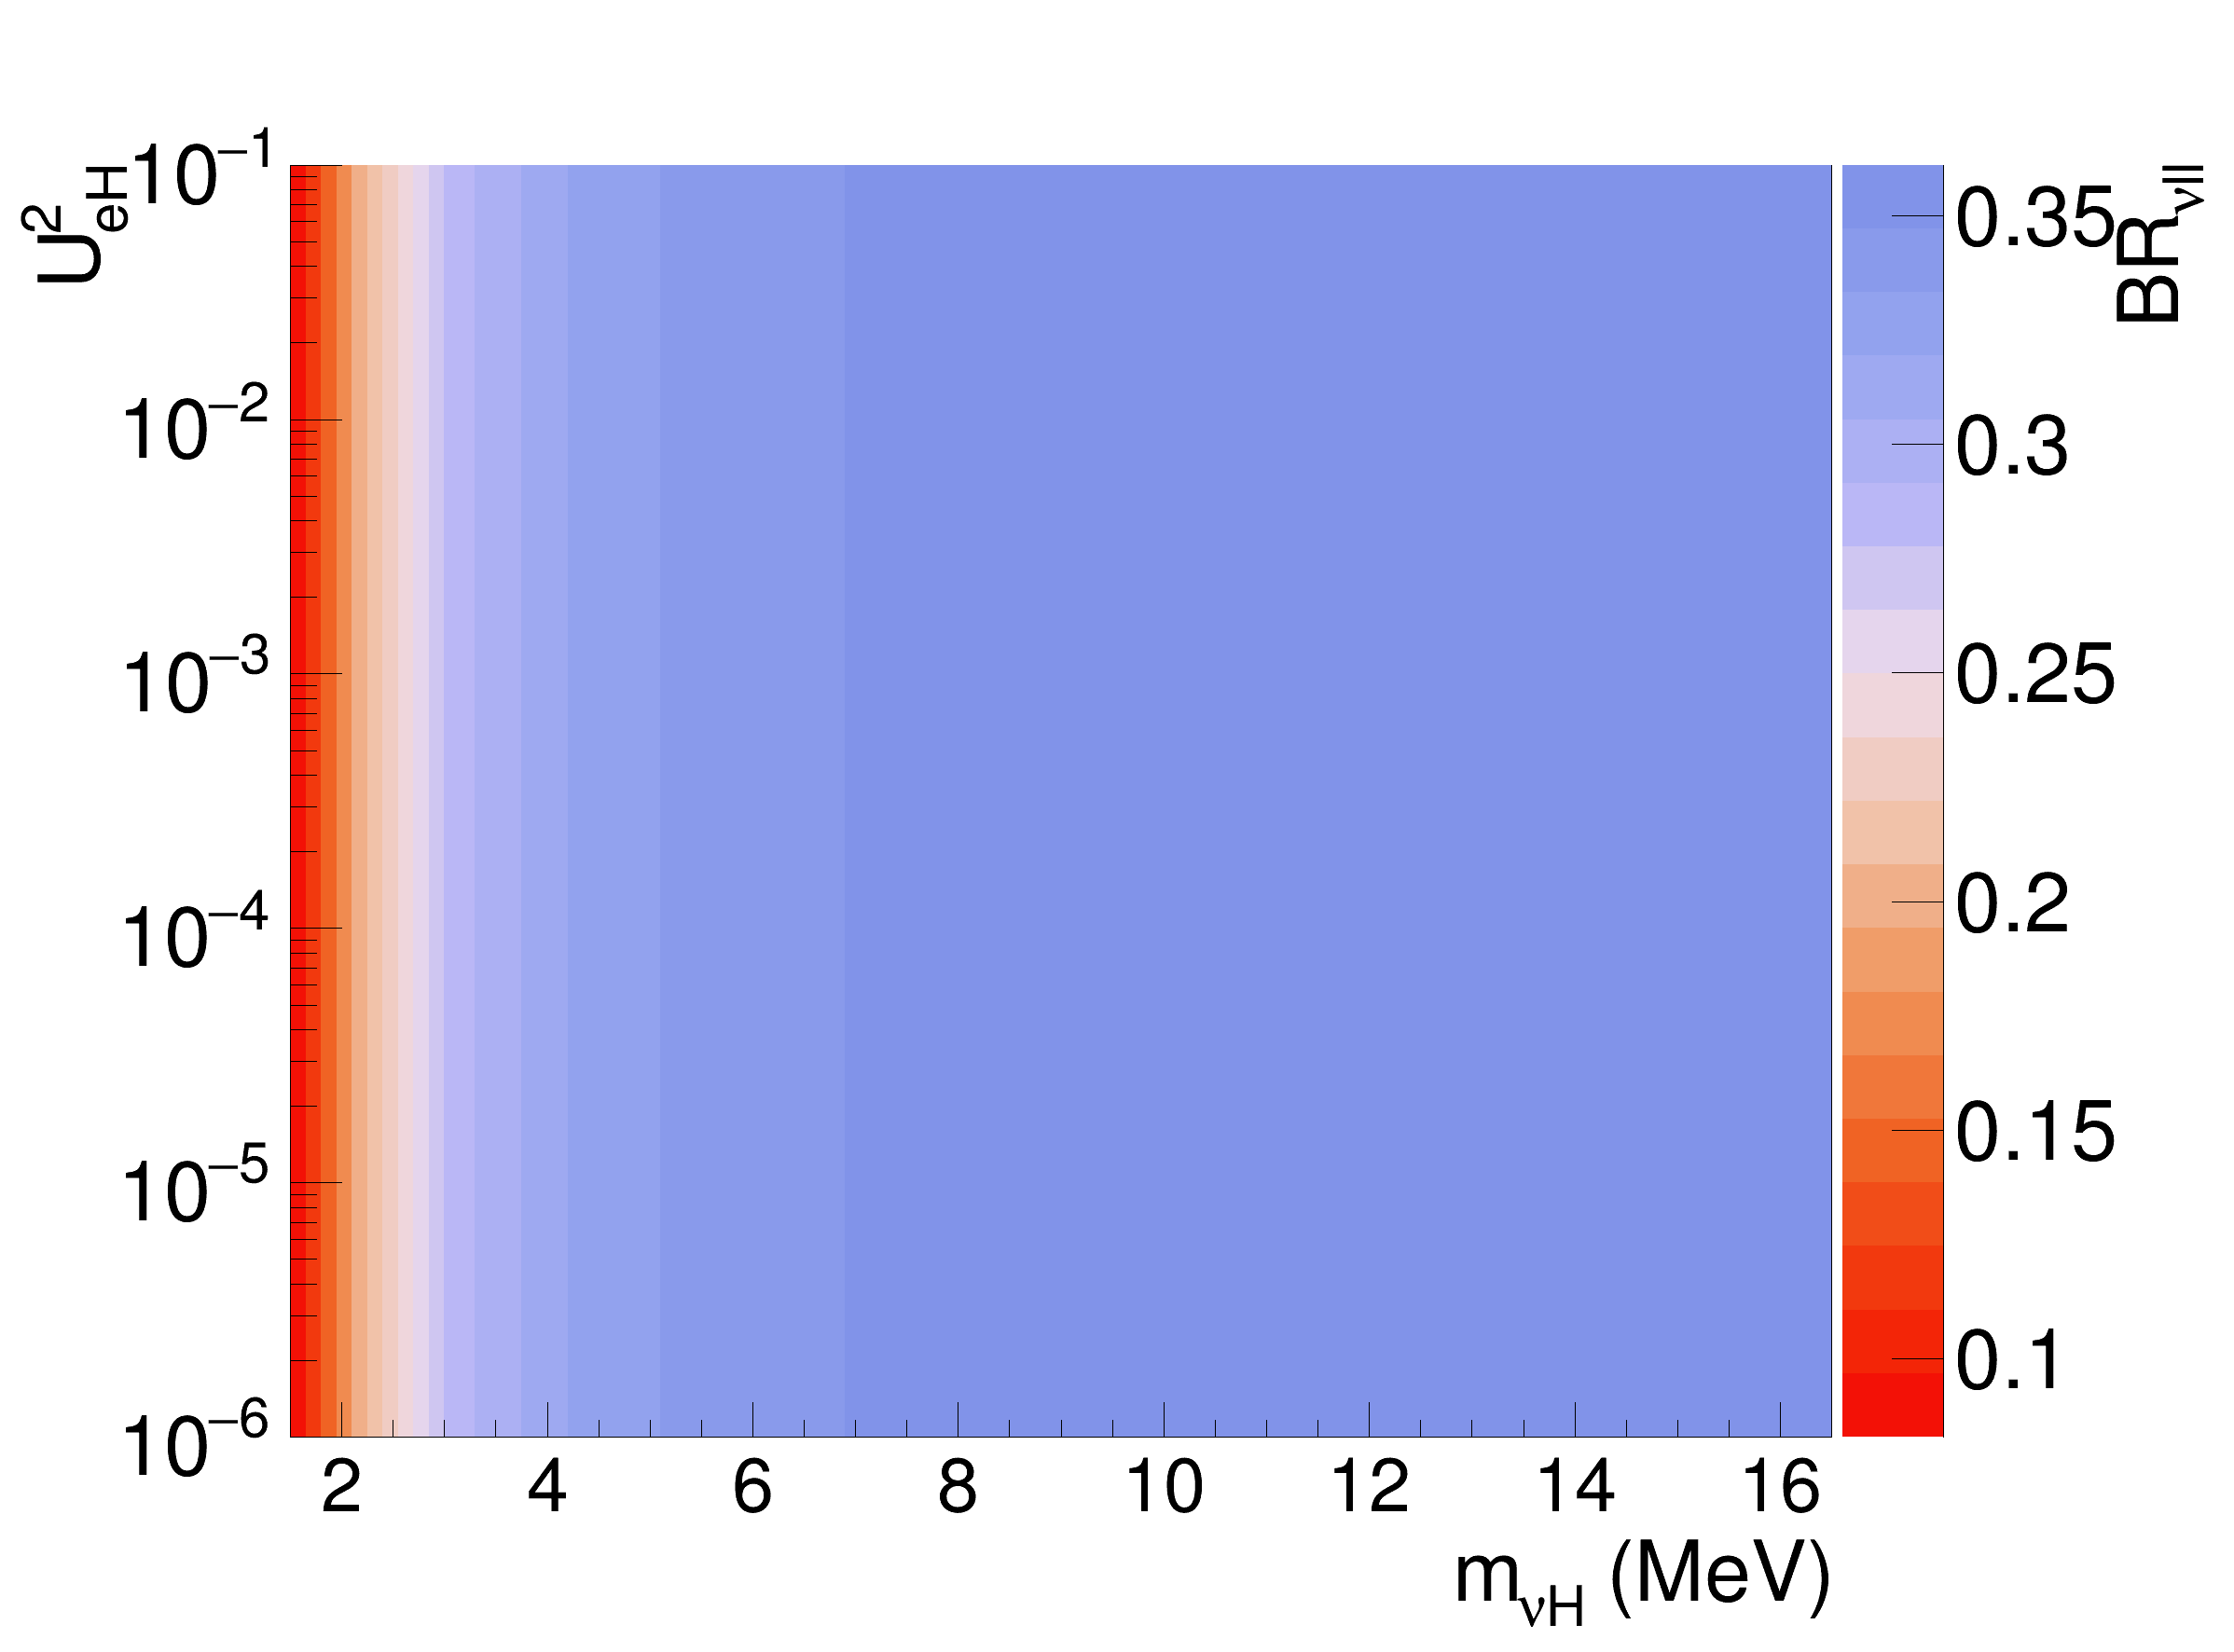
\includegraphics[width=0.99\columnwidth]{../plots/RHNBRvll_vs_M_U2_linXlogYlinZ.png}
\caption{Branching ratio of $\nu_H$ decay to $\nu_e e^+ e^-$ for different masses and different mixing parameter $|U_{eH}|^2$. }
\label{fig:RHNBRvll} 
\end{figure}


\begin{figure}[!htbp]
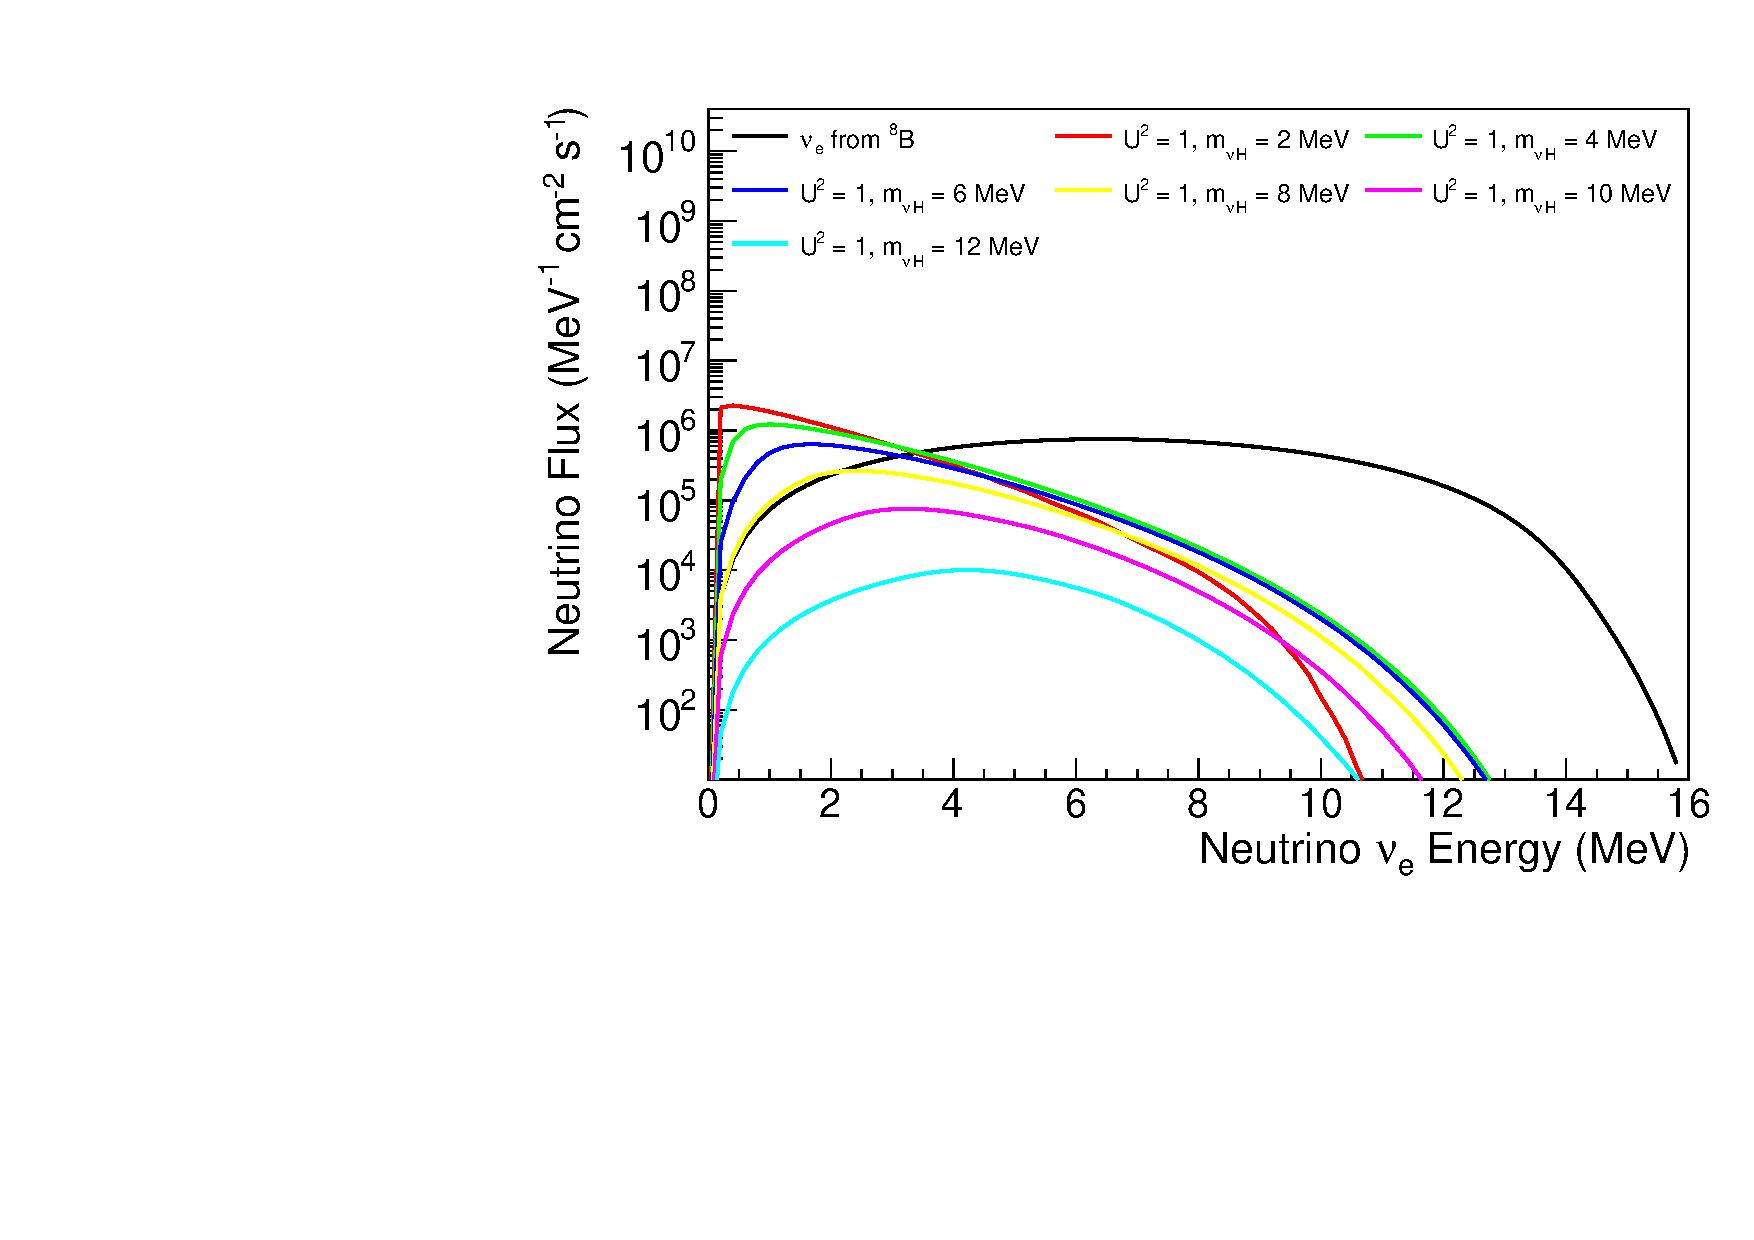
\includegraphics[width=0.99\columnwidth]{../plots/nuLSpectrum_U1.0_AllMass_linXlogY.pdf}
\caption{Energy spectra of left-handed neutrinos ($\nu_e$) in the lab frame from $\nu_H$ to $\nu_e e^+ e^-$ decay for different $\nu_H$ masses. The spectra shown in this plot include all $\nu_H$ decay (regardless of where they decay). The original solar neutrino energy spectrum from  $^8B$ in the Sun is also shown in the plot (black curve). }
\label{fig:nuLSpectrum_all_decay} 
\end{figure}

\begin{figure}[!htbp]
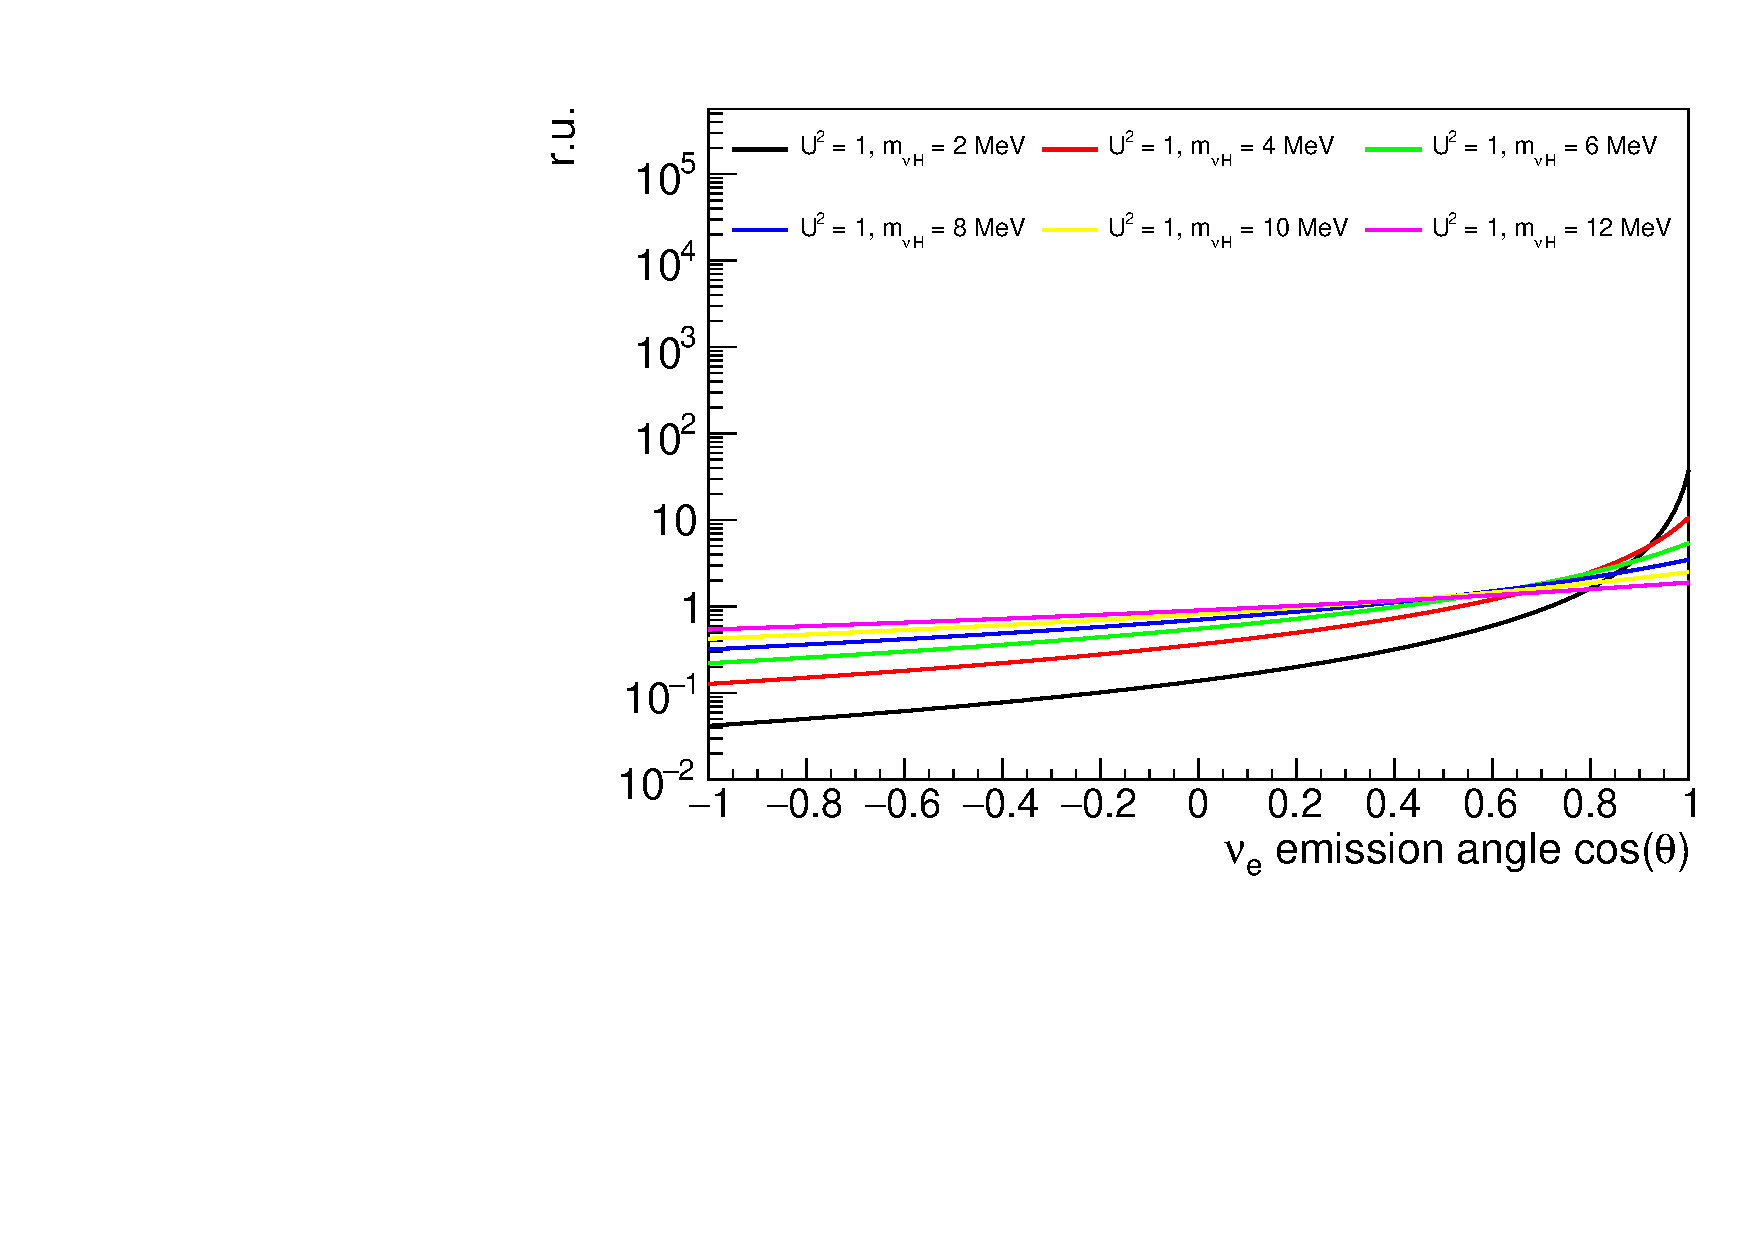
\includegraphics[width=0.99\columnwidth]{../plots/nuLEmissionAngle_U1.0_AllMass_linXlogY.pdf}\\
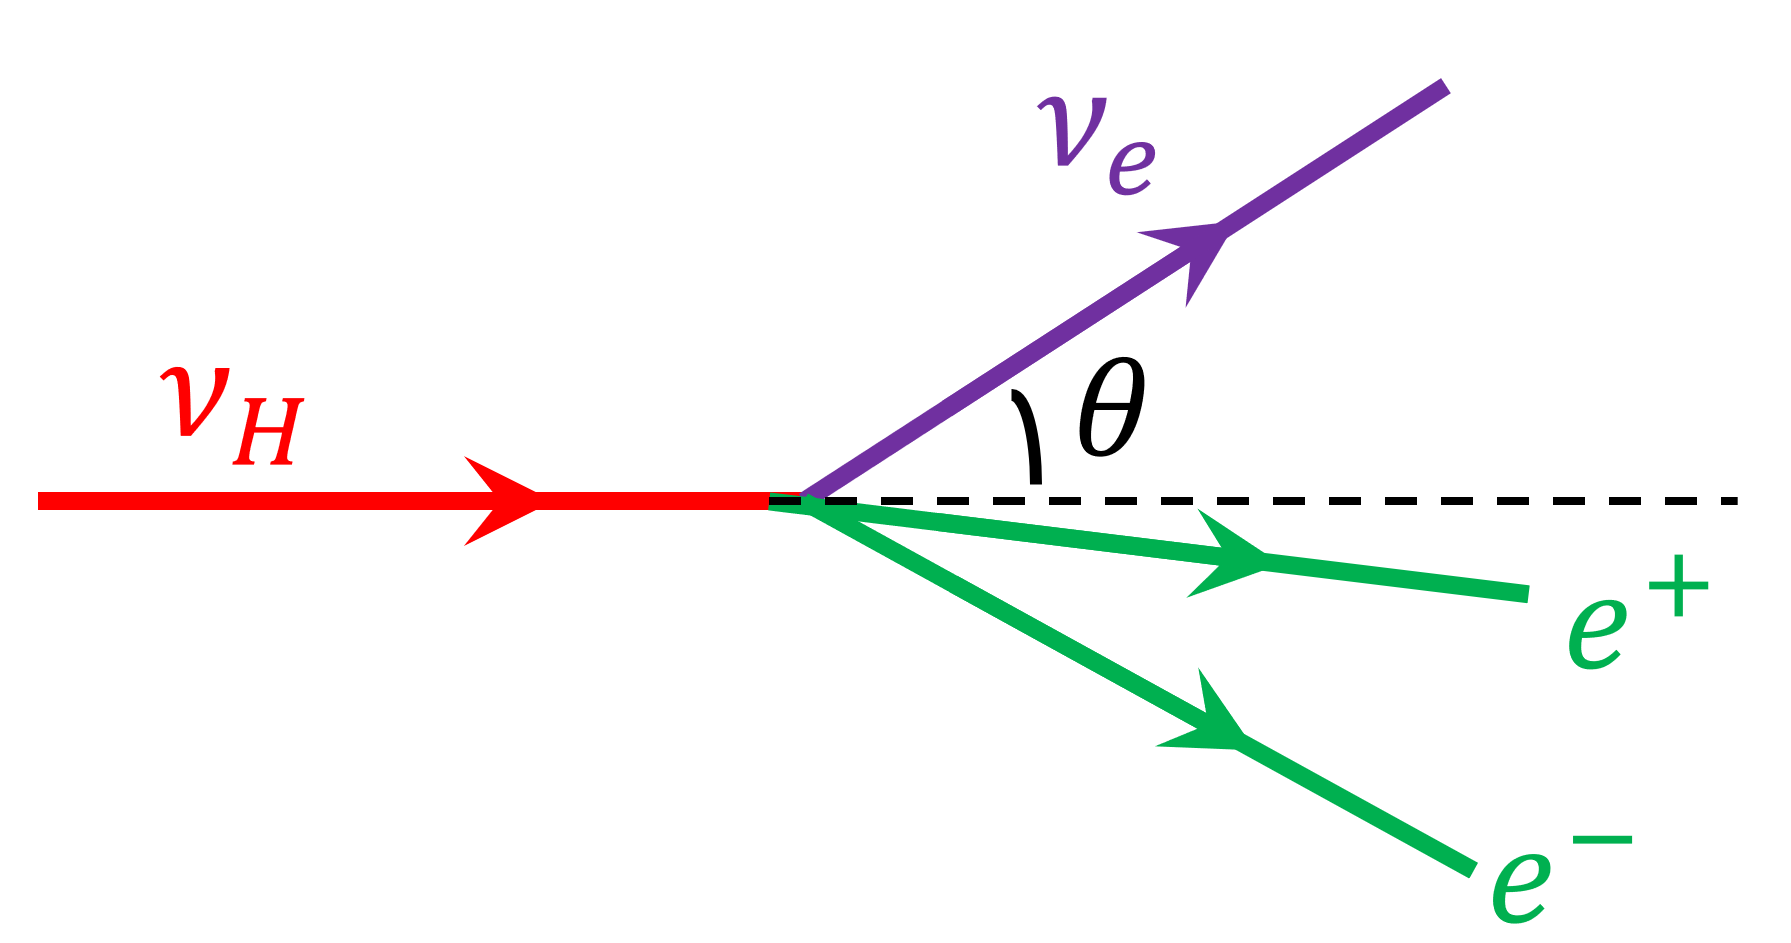
\includegraphics[width=0.7\columnwidth]{figs/emission_angle_sketch.png}
\caption{Top: emission angle $\cos(\theta)$ distribution of left-handed neutrinos ($\nu_e$) in the lab frame from $\nu_H$ to $\nu_e e^+ e^-$ decay for different $\nu_H$ masses. The plots shown in this plot include all $\nu_H$ decay (regardless of where they decay). Bottom: sketch of definition of emission angle $\theta$.}
\label{fig:nuLEmissionAngle_all_decay} 
\end{figure}

\clearpage
\section{\label{sec:EeSpectrum} Search for $\nu_H$ with $e^+e^-$ spectrum}

\begin{figure}[!htbp]
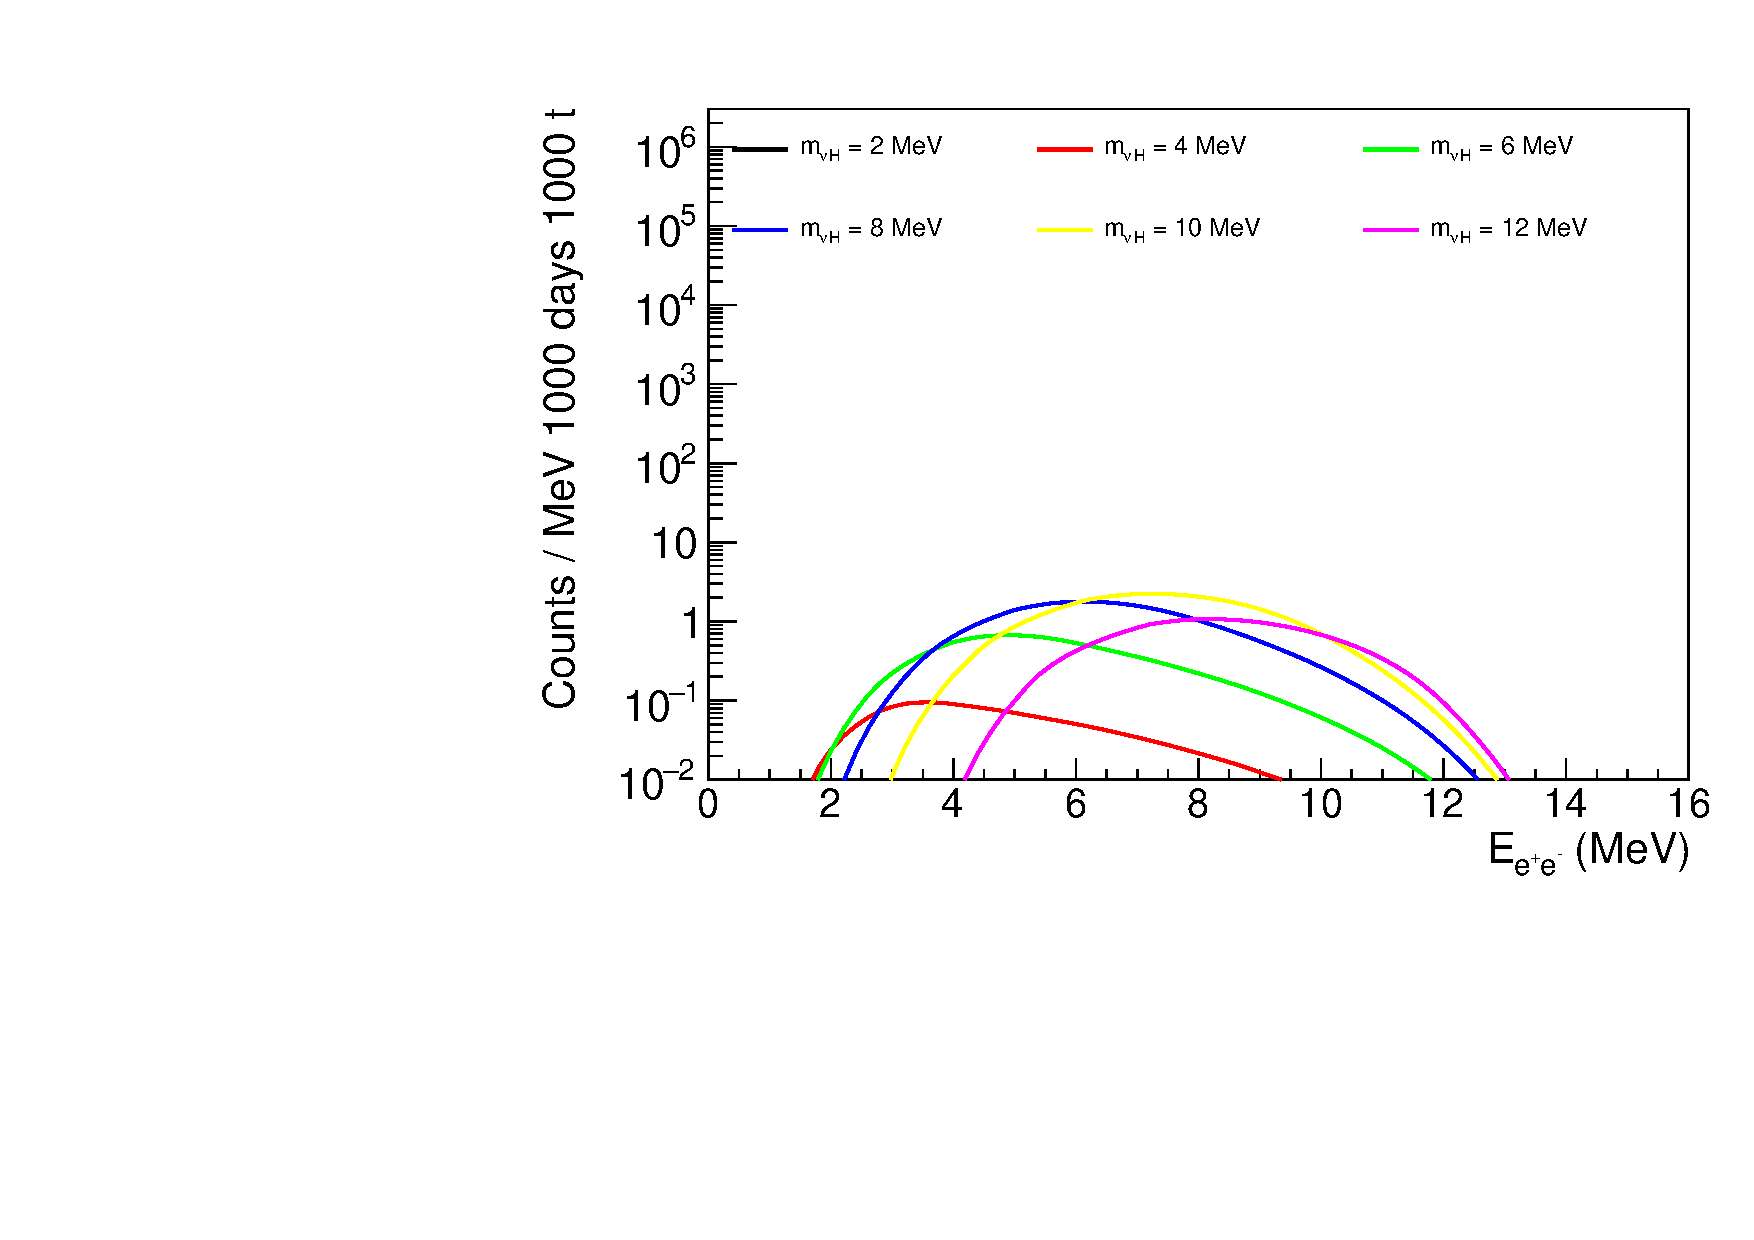
\includegraphics[width=0.99\columnwidth]{../plots/EeeSpectrum_decay_in_detector_integrate_U1e-06_AllMass_linXlogY.pdf}
\caption{The expected energy spectra of of $e^+e^-$ pairs in the lab frame from $\nu_H$ to $\nu_e e^+ e^-$ decay for  different $\nu_H$ masses. 
The spectra only include $\nu_H$'s that decay inside a 1000-ton detector placed on earth over 1000 days. 
The mixing parameter $|U_{eH}|^2$ is  $10^{-6}$ in this plot.}
\label{fig:EeeSpectrum_in_detector_U1em6} 
\end{figure}

\begin{figure}[!htbp]
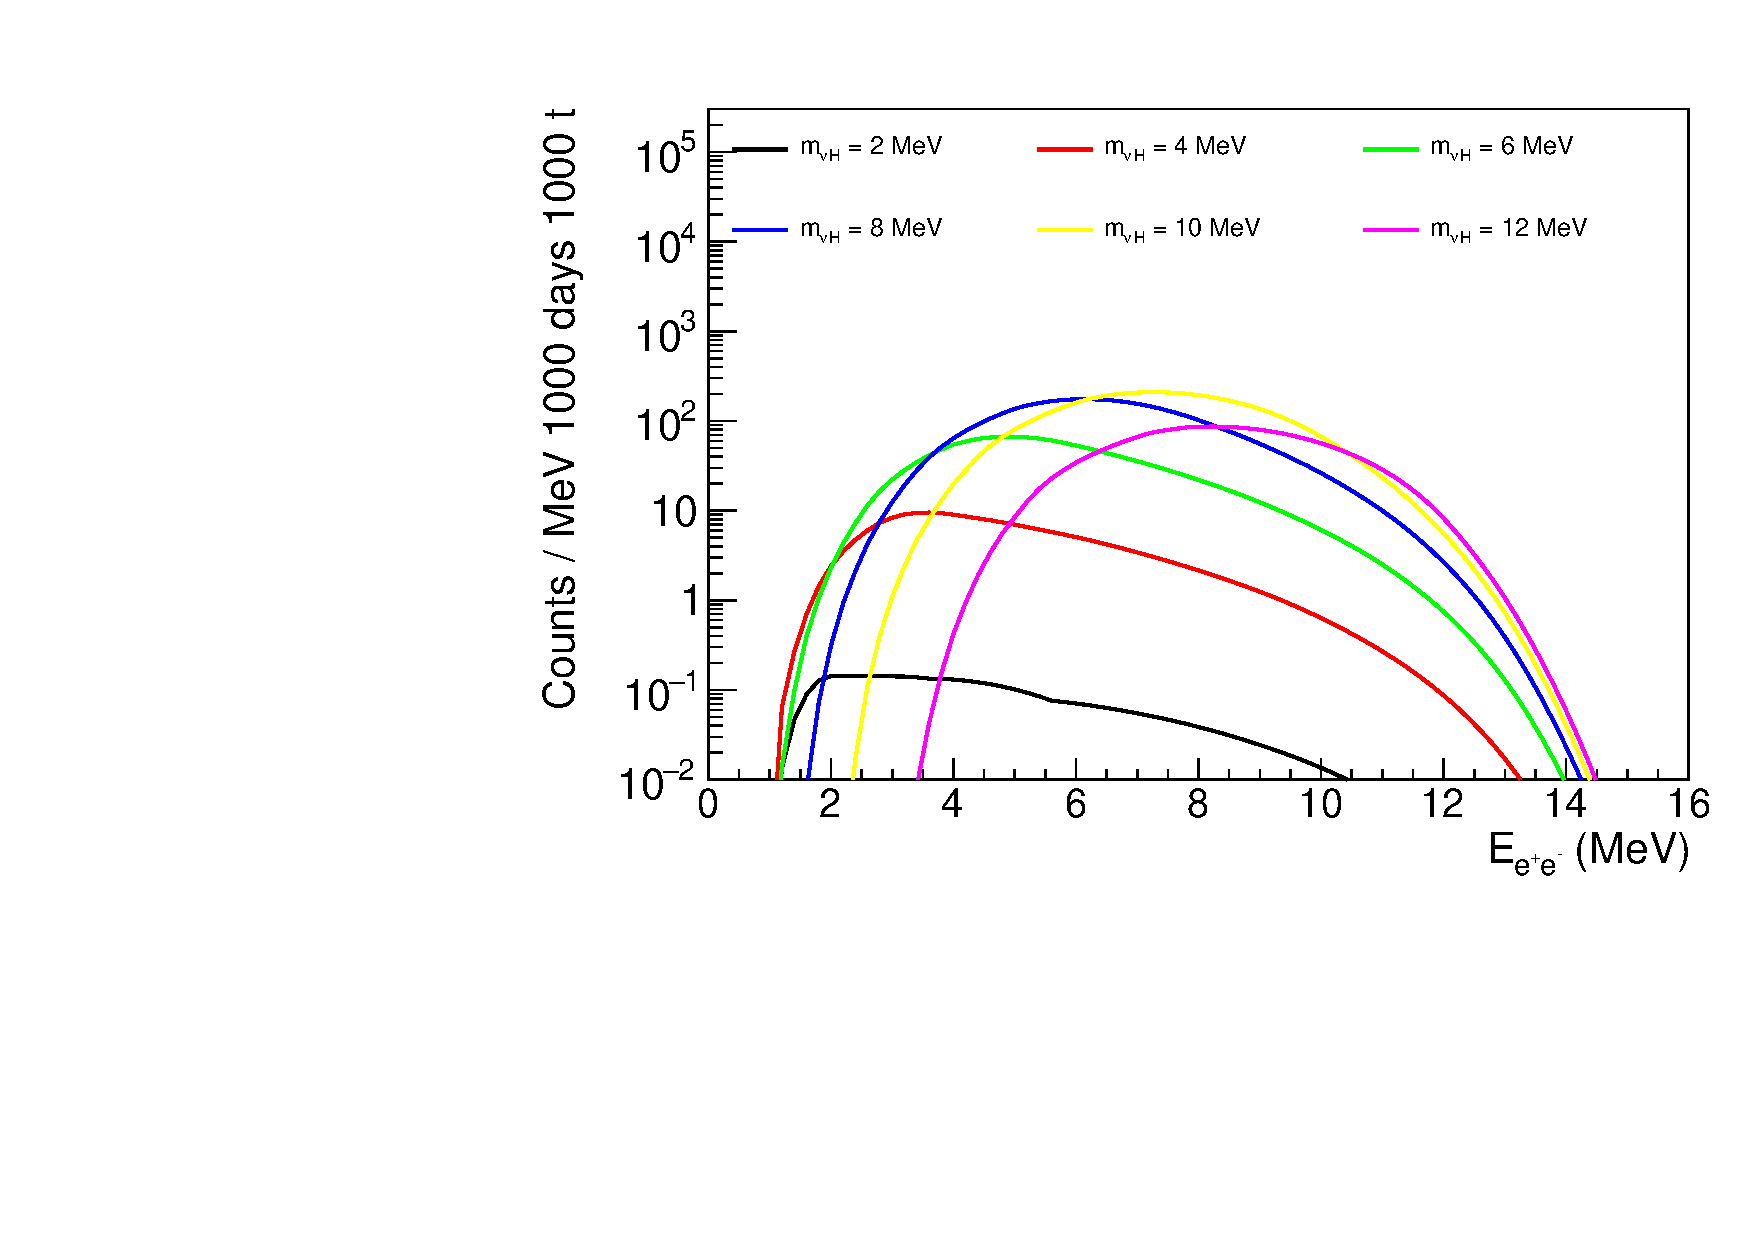
\includegraphics[width=0.99\columnwidth]{../plots/EeeSpectrum_decay_in_detector_integrate_U1e-05_AllMass_linXlogY.pdf}
\caption{The expected energy spectra of of $e^+e^-$ pairs in the lab frame from $\nu_H$ to $\nu_e e^+ e^-$ decay for  different $\nu_H$ masses. 
The spectra only include $\nu_H$'s that decay inside a 1000-ton detector placed on earth over 1000 days. 
The mixing parameter $|U_{eH}|^2$ is  $10^{-5}$ in this plot.}
\label{fig:EeeSpectrum_in_detector_U1em5} 
\end{figure}

\begin{figure}[!htbp]
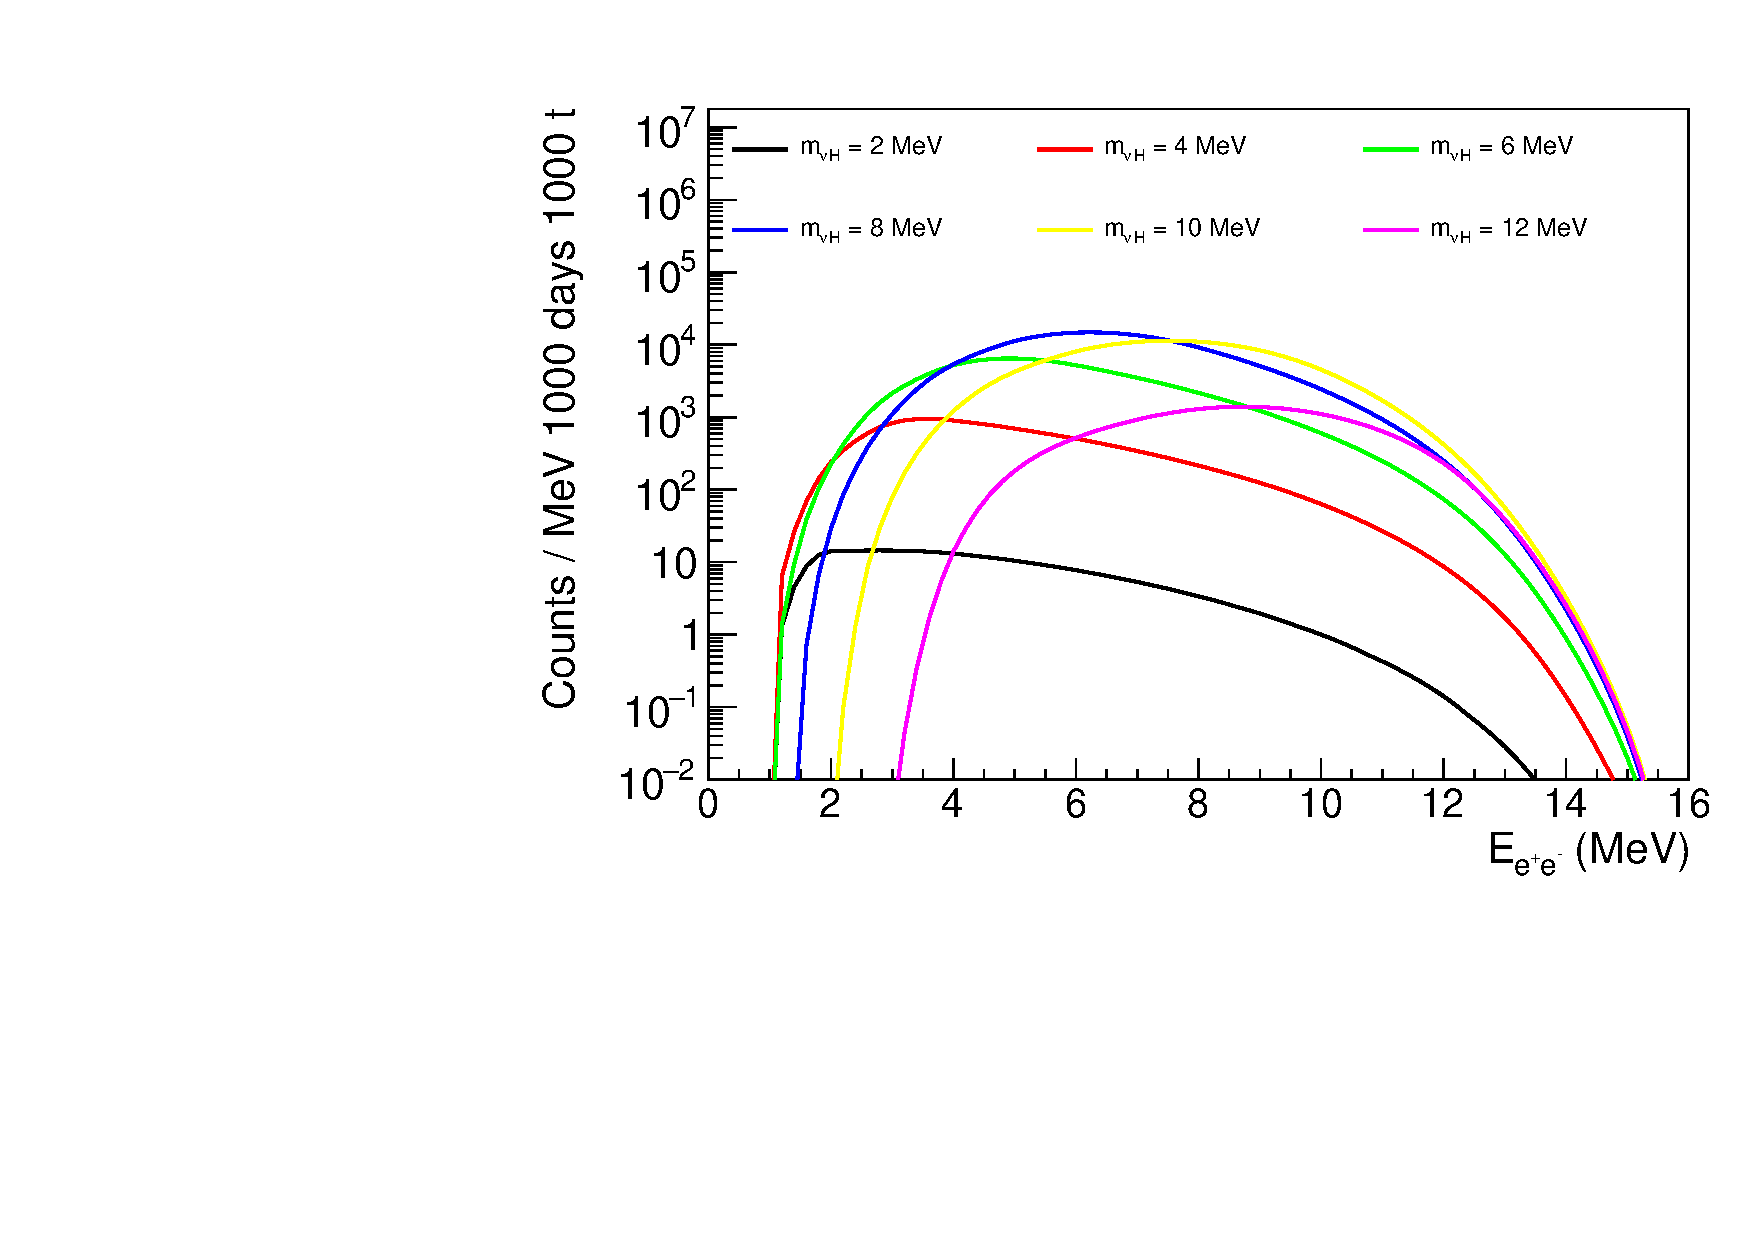
\includegraphics[width=0.99\columnwidth]{../plots/EeeSpectrum_decay_in_detector_integrate_U0.0001_AllMass_linXlogY.pdf}
\caption{The expected energy spectra of of $e^+e^-$ pairs in the lab frame from $\nu_H$ to $\nu_e e^+ e^-$ decay for  different $\nu_H$ masses. 
The spectra only include $\nu_H$'s that decay inside a 1000-ton detector placed on earth over 1000 days. 
The mixing parameter $|U_{eH}|^2$ is  $10^{-4}$ in this plot.}
\label{fig:EeeSpectrum_in_detector_U1em4} 
\end{figure}

\begin{figure}[!htbp]
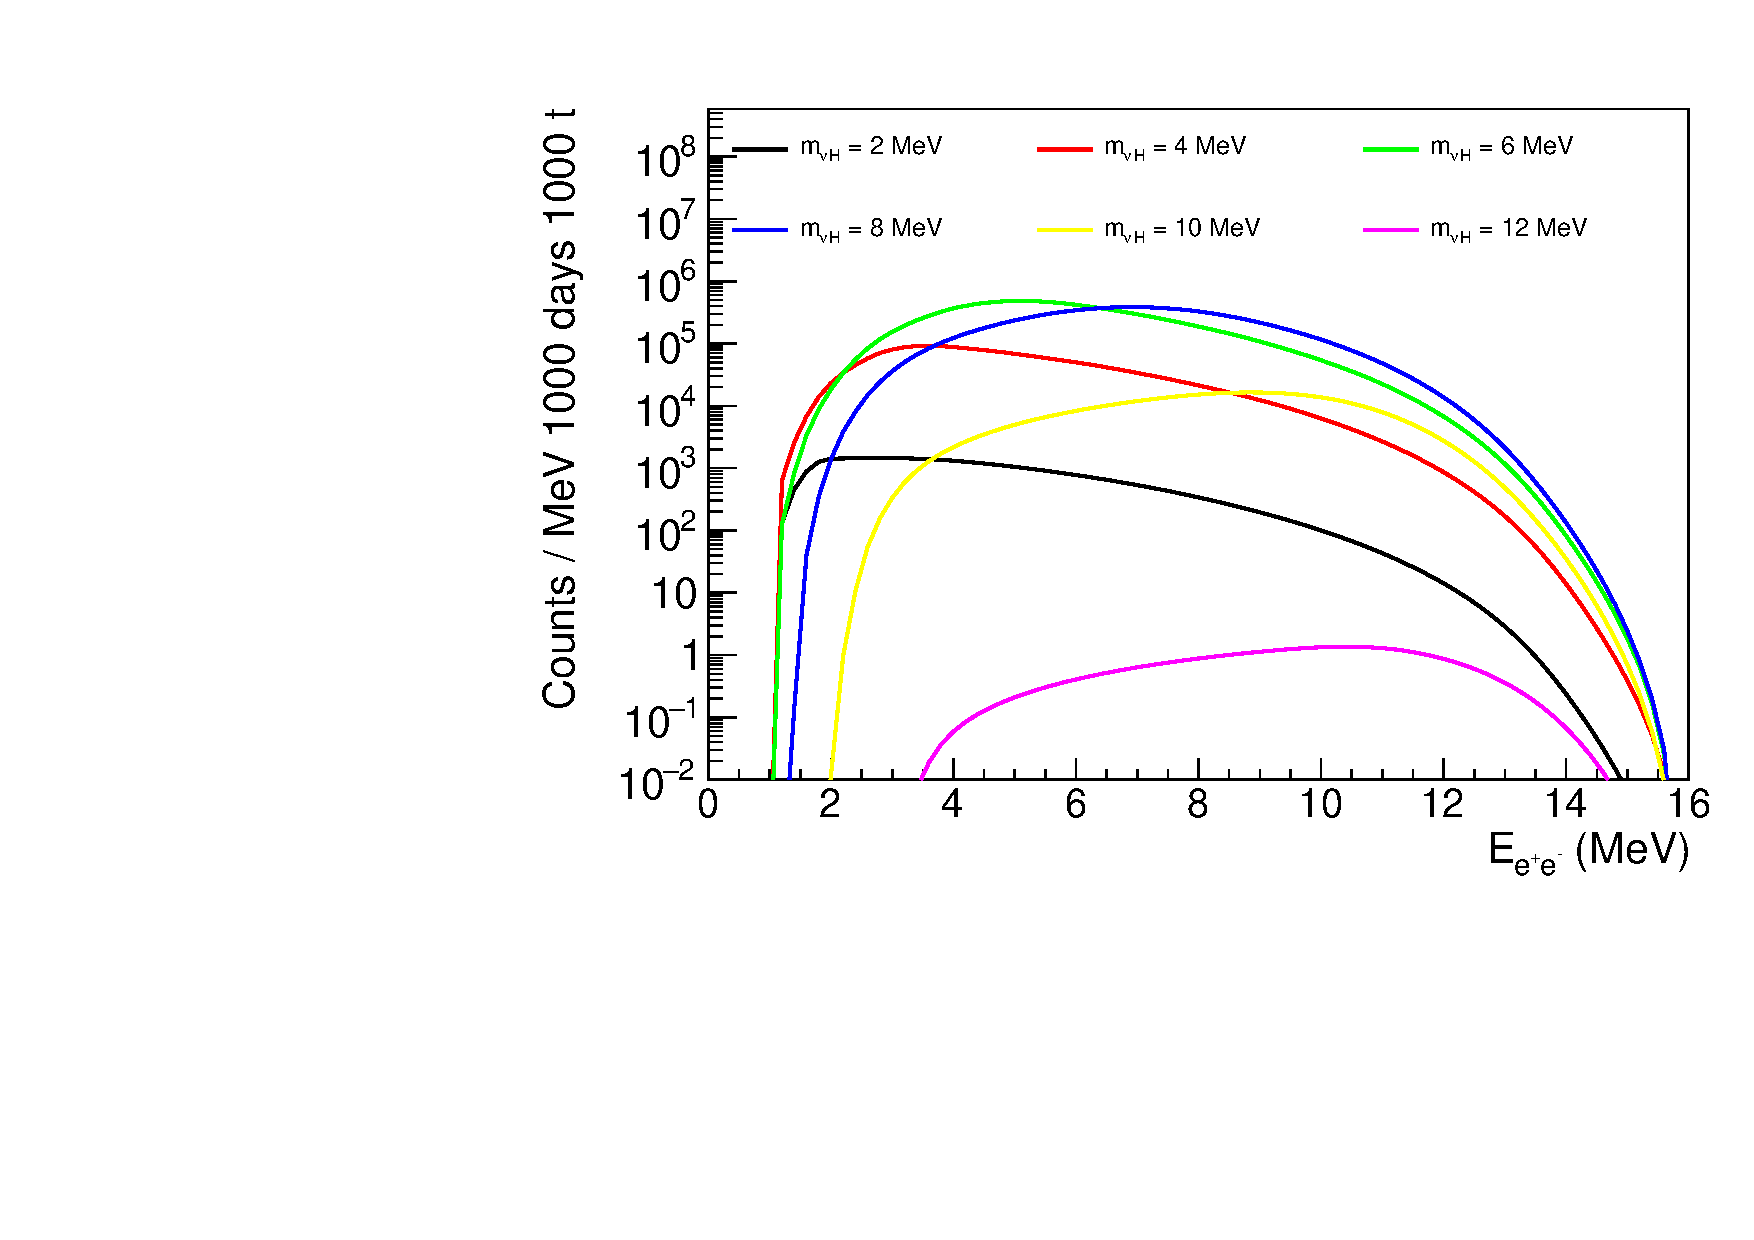
\includegraphics[width=0.99\columnwidth]{../plots/EeeSpectrum_decay_in_detector_integrate_U0.001_AllMass_linXlogY.pdf}
\caption{The expected energy spectra of of $e^+e^-$ pairs in the lab frame from $\nu_H$ to $\nu_e e^+ e^-$ decay for  different $\nu_H$ masses. 
The spectra only include $\nu_H$'s that decay inside a 1000-ton detector placed on earth over 1000 days. 
The mixing parameter $|U_{eH}|^2$ is  $10^{-3}$ in this plot.}
\label{fig:EeeSpectrum_in_detector_U1em3} 
\end{figure}

\begin{figure}[!htbp]
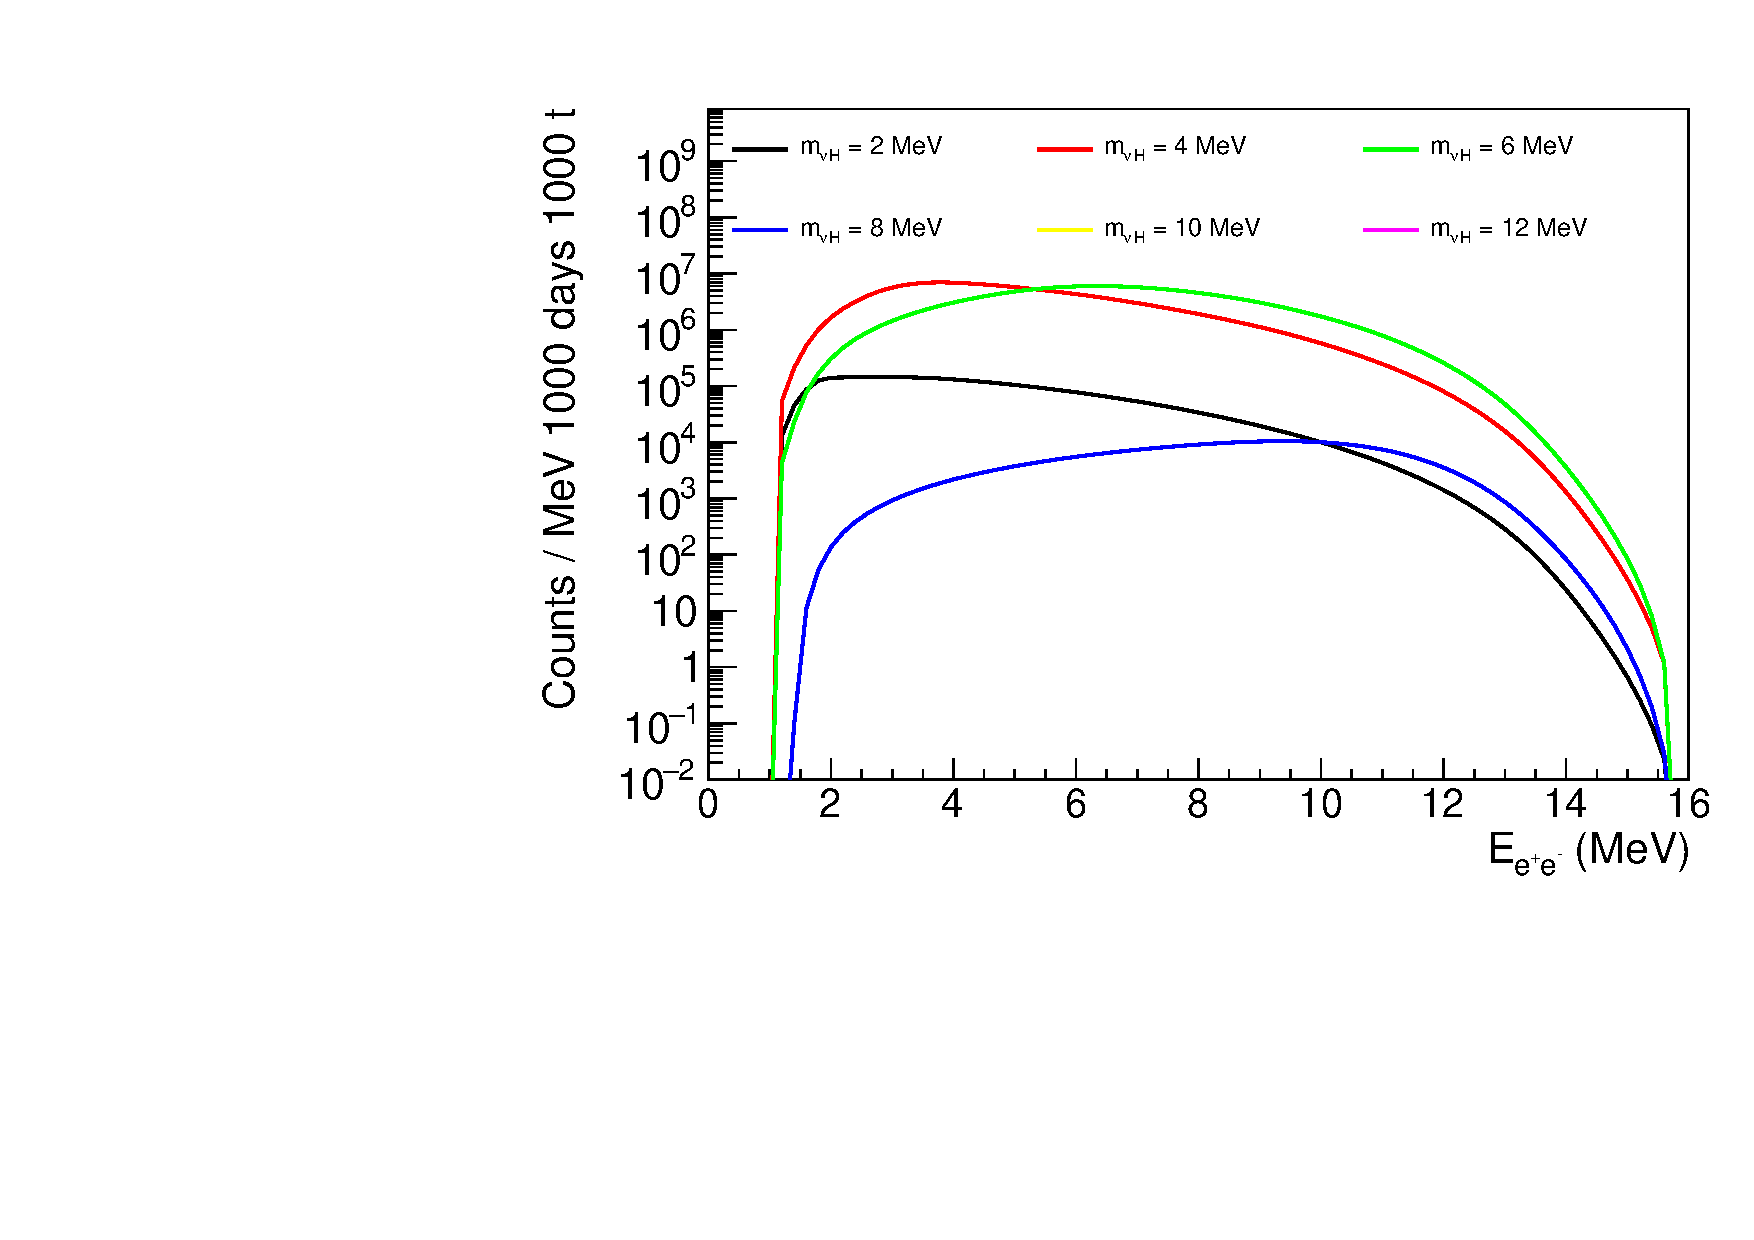
\includegraphics[width=0.99\columnwidth]{../plots/EeeSpectrum_decay_in_detector_integrate_U0.01_AllMass_linXlogY.pdf}
\caption{The expected energy spectra of of $e^+e^-$ pairs in the lab frame from $\nu_H$ to $\nu_e e^+ e^-$ decay for  different $\nu_H$ masses. 
The spectra only include $\nu_H$'s that decay inside a 1000-ton detector placed on earth over 1000 days. 
The mixing parameter $|U_{eH}|^2$ is  $10^{-2}$ in this plot.}
\label{fig:EeeSpectrum_in_detector_U1em2} 
\end{figure}

\begin{figure}[!htbp]
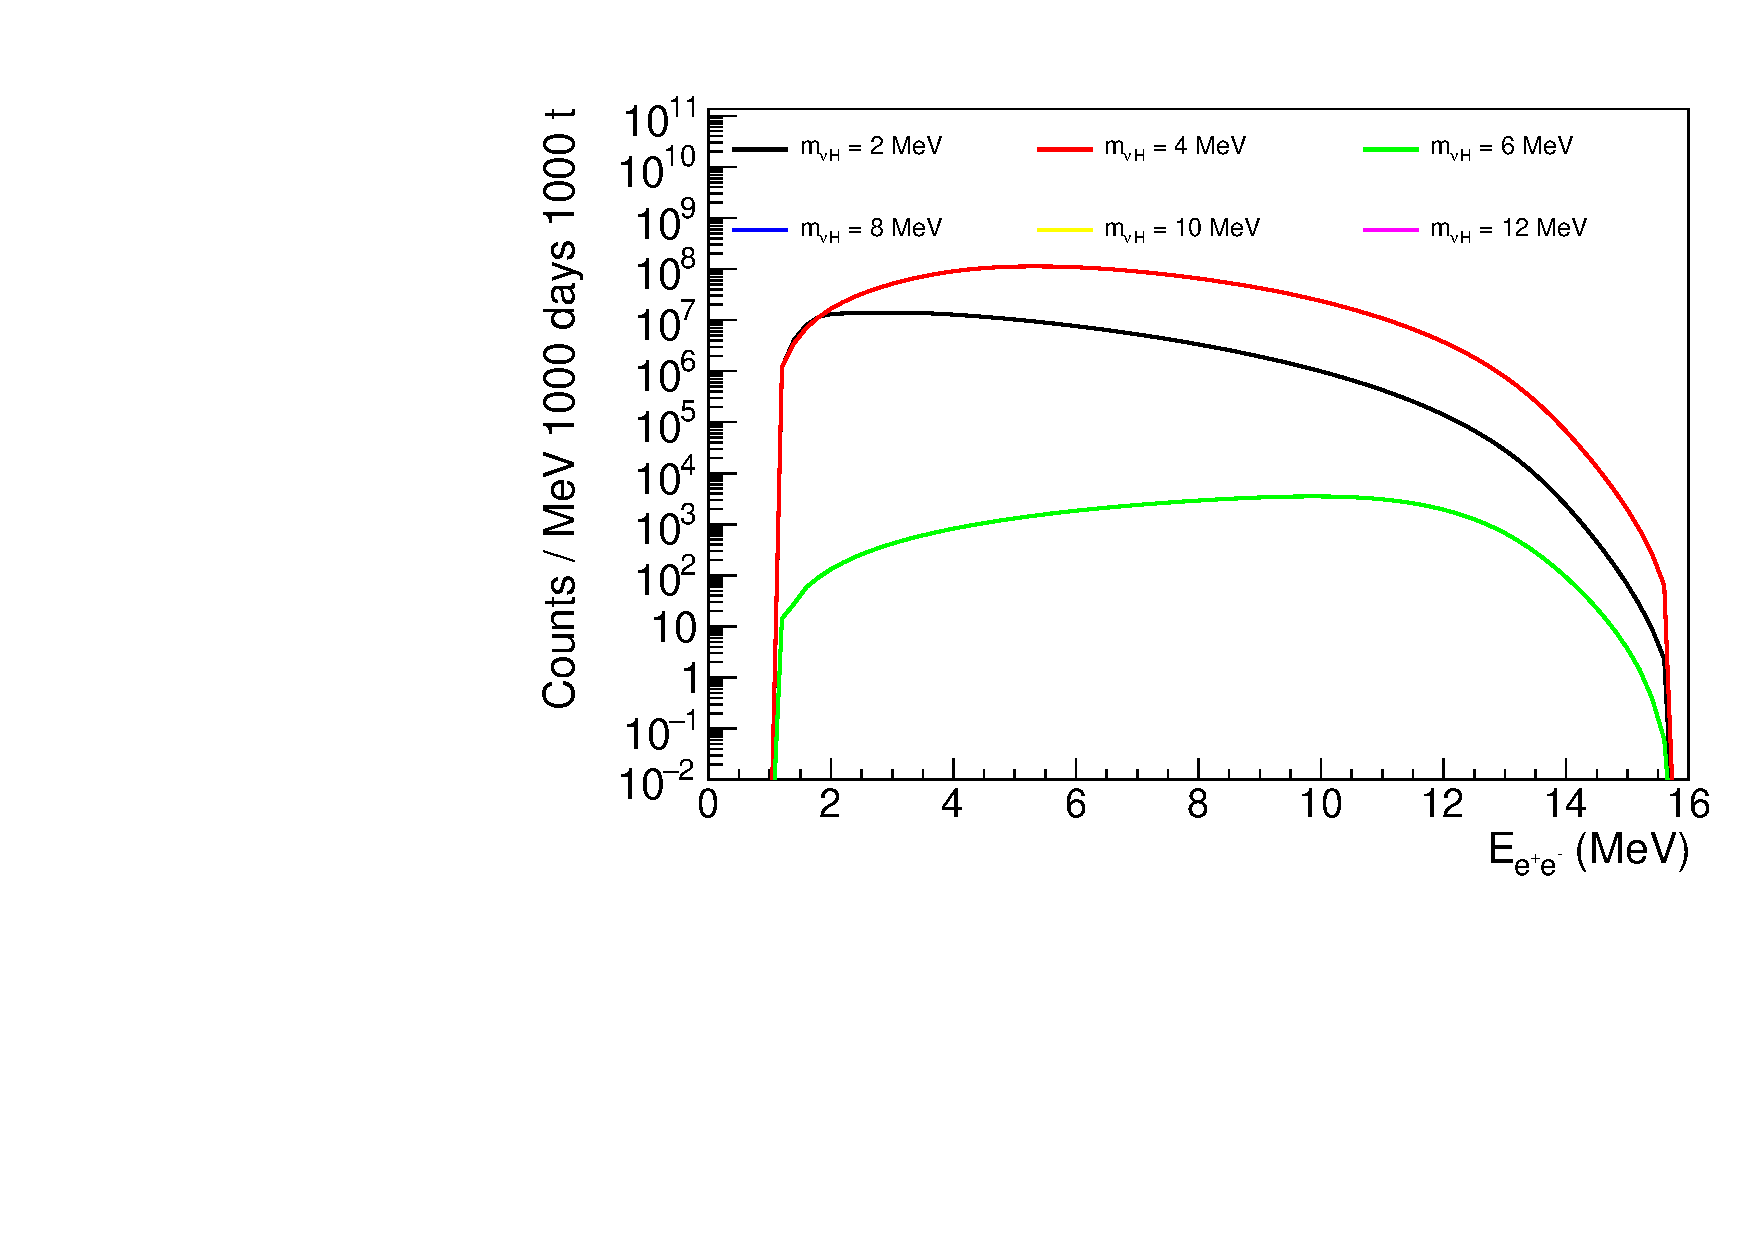
\includegraphics[width=0.99\columnwidth]{../plots/EeeSpectrum_decay_in_detector_integrate_U0.1_AllMass_linXlogY.pdf}
\caption{The expected energy spectra of of $e^+e^-$ pairs in the lab frame from $\nu_H$ to $\nu_e e^+ e^-$ decay for  different $\nu_H$ masses. 
The spectra only include $\nu_H$'s that decay inside a 1000-ton detector placed on earth over 1000 days. 
The mixing parameter $|U_{eH}|^2$ is  $10^{-1}$ in this plot.}
\label{fig:EeeSpectrum_in_detector_U1em1} 
\end{figure}

\begin{figure}[!htbp]
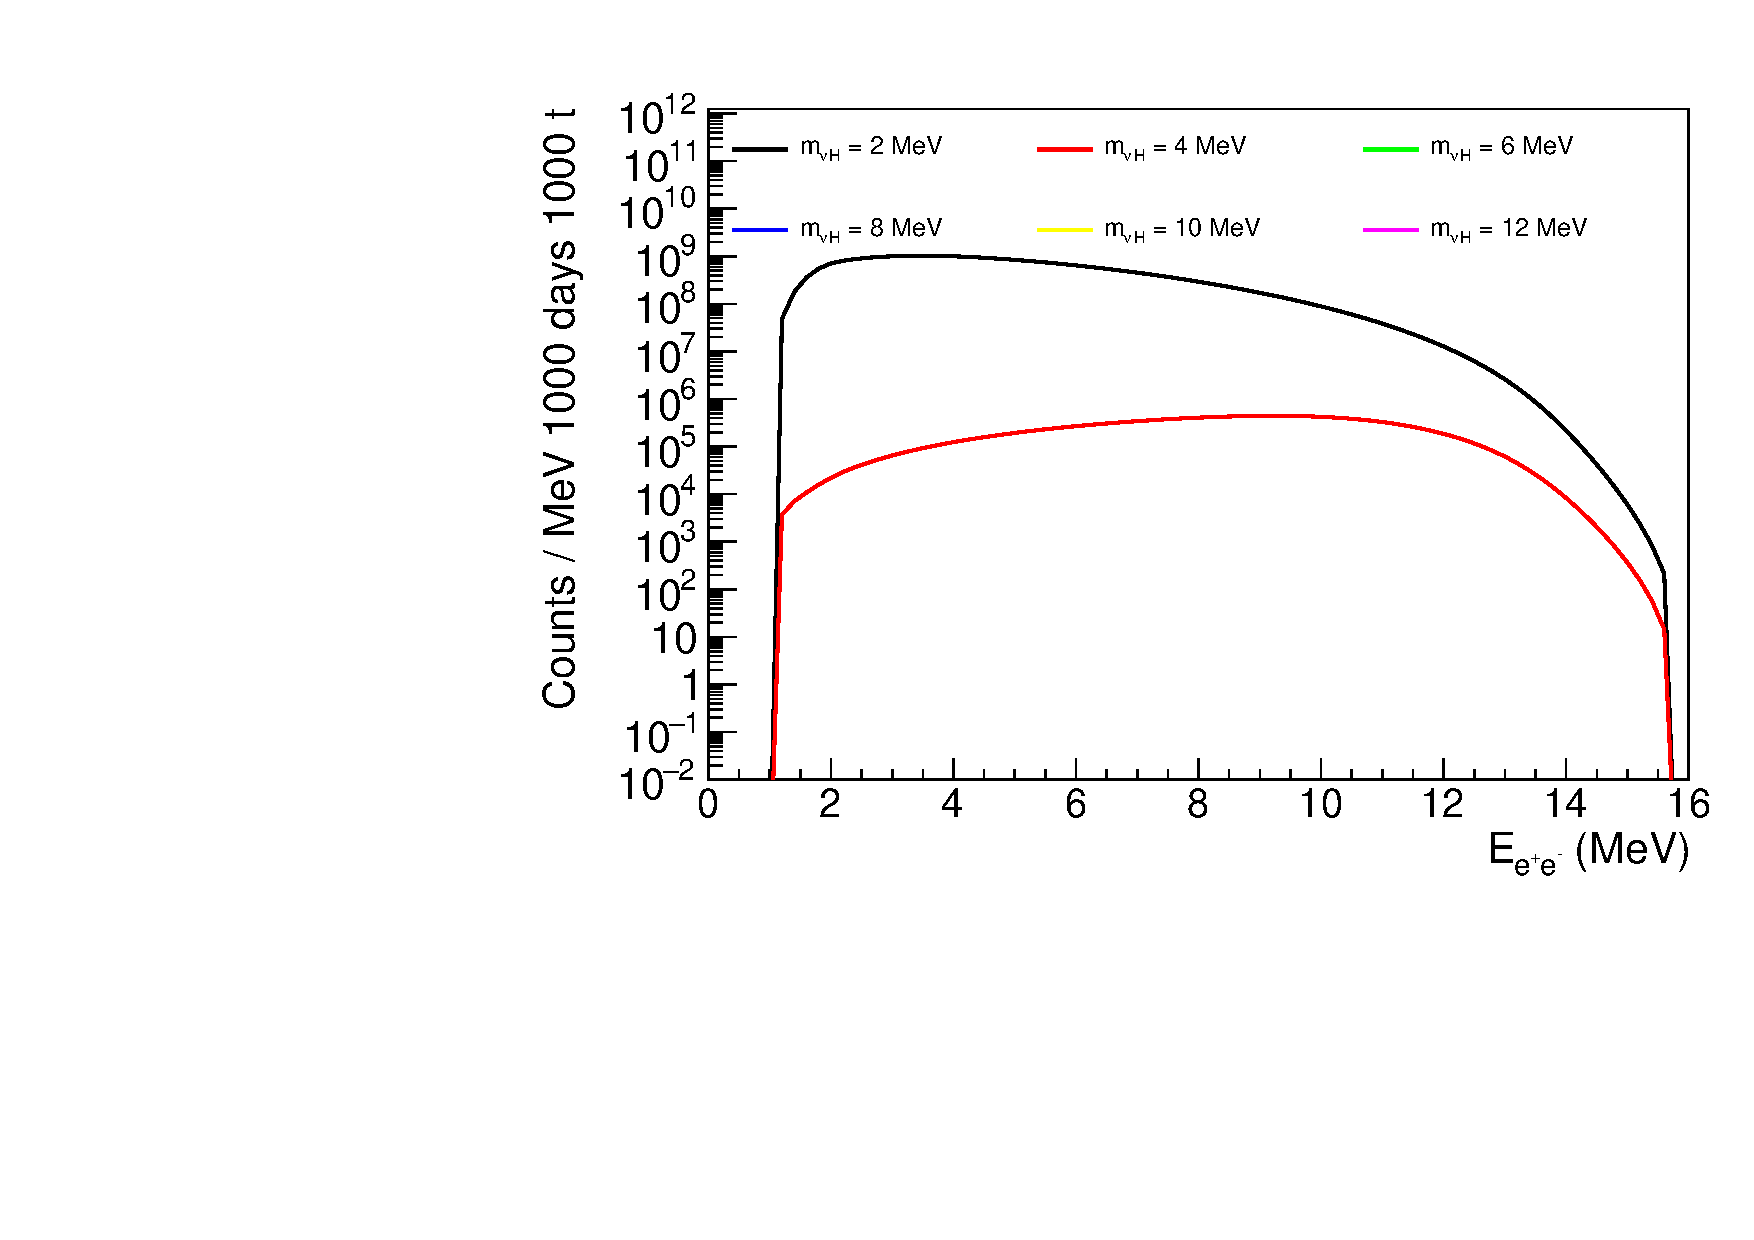
\includegraphics[width=0.99\columnwidth]{../plots/EeeSpectrum_decay_in_detector_integrate_U1.0_AllMass_linXlogY.pdf}
\caption{The expected energy spectra of of $e^+e^-$ pairs in the lab frame from $\nu_H$ to $\nu_e e^+ e^-$ decay for  different $\nu_H$ masses. 
The spectra only include $\nu_H$'s that decay inside a 1000-ton detector placed on earth over 1000 days. 
The mixing parameter $|U_{eH}|^2$ is  $1.0$ in this plot.}
\label{fig:EeeSpectrum_in_detector_U1em0} 
\end{figure}

\clearpage
\section{\label{sec:NueAngle} Search for $\nu_H$ with $\nu_e$ solar angle}

\begin{figure}[!htbp]
    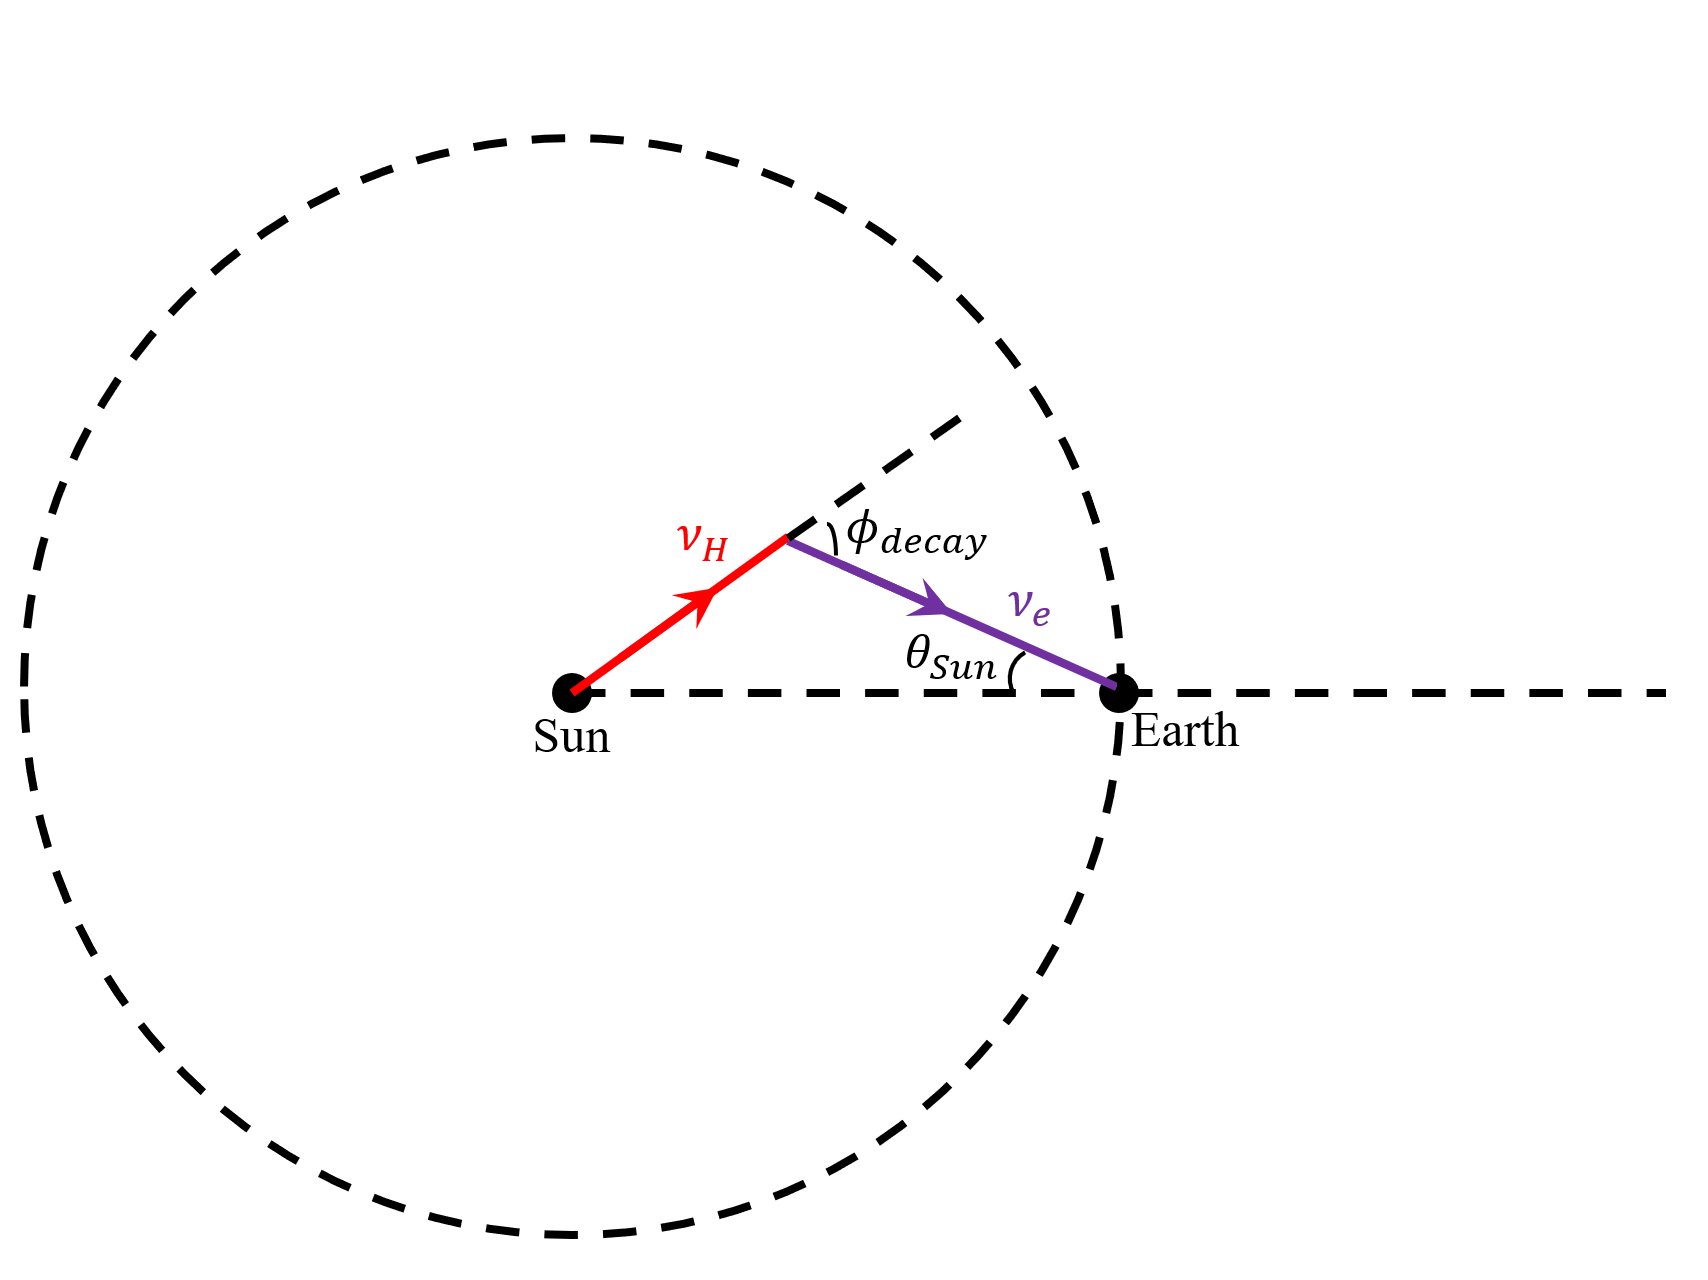
\includegraphics[width=0.55\columnwidth]{figs/decay_inflight_sketch1.png}\\
    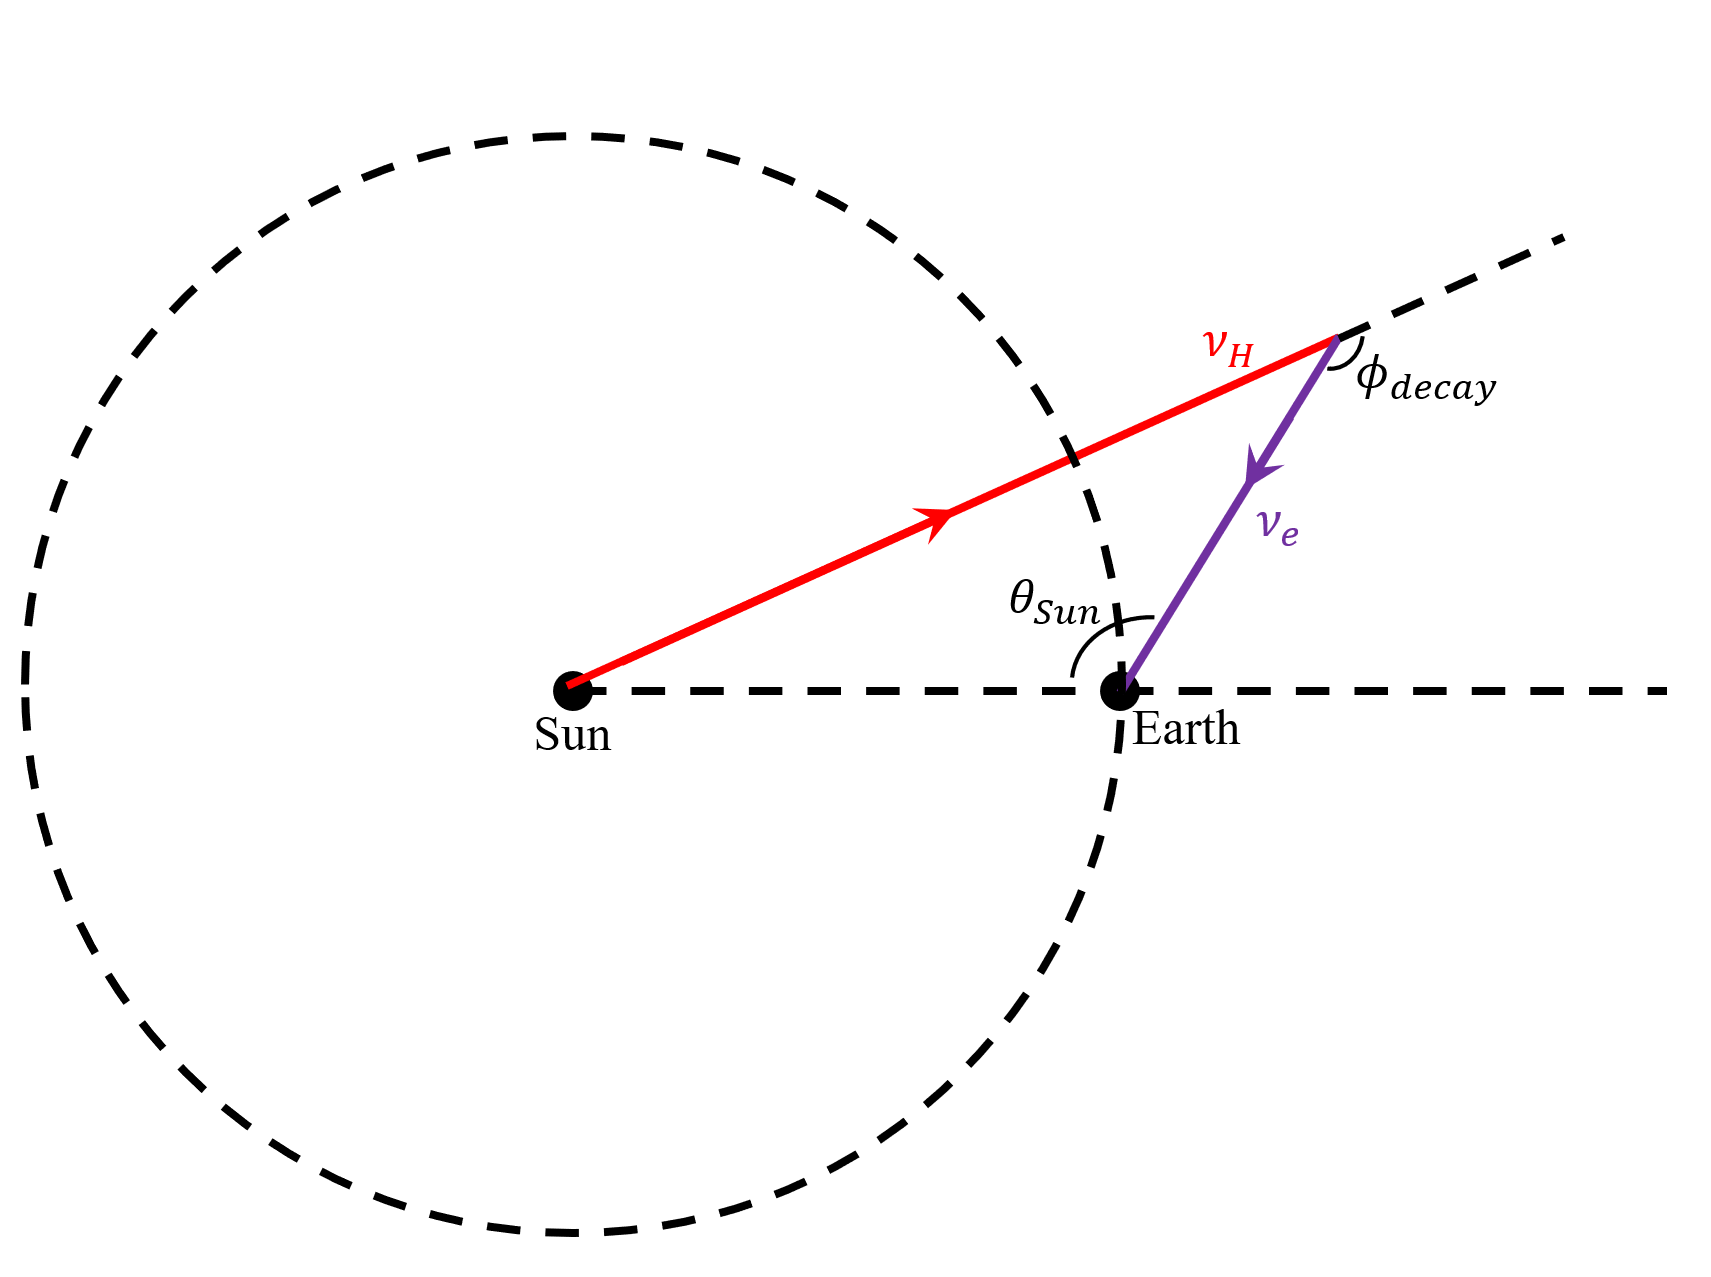
\includegraphics[width=0.45\columnwidth]{figs/decay_inflight_sketch2.png}
    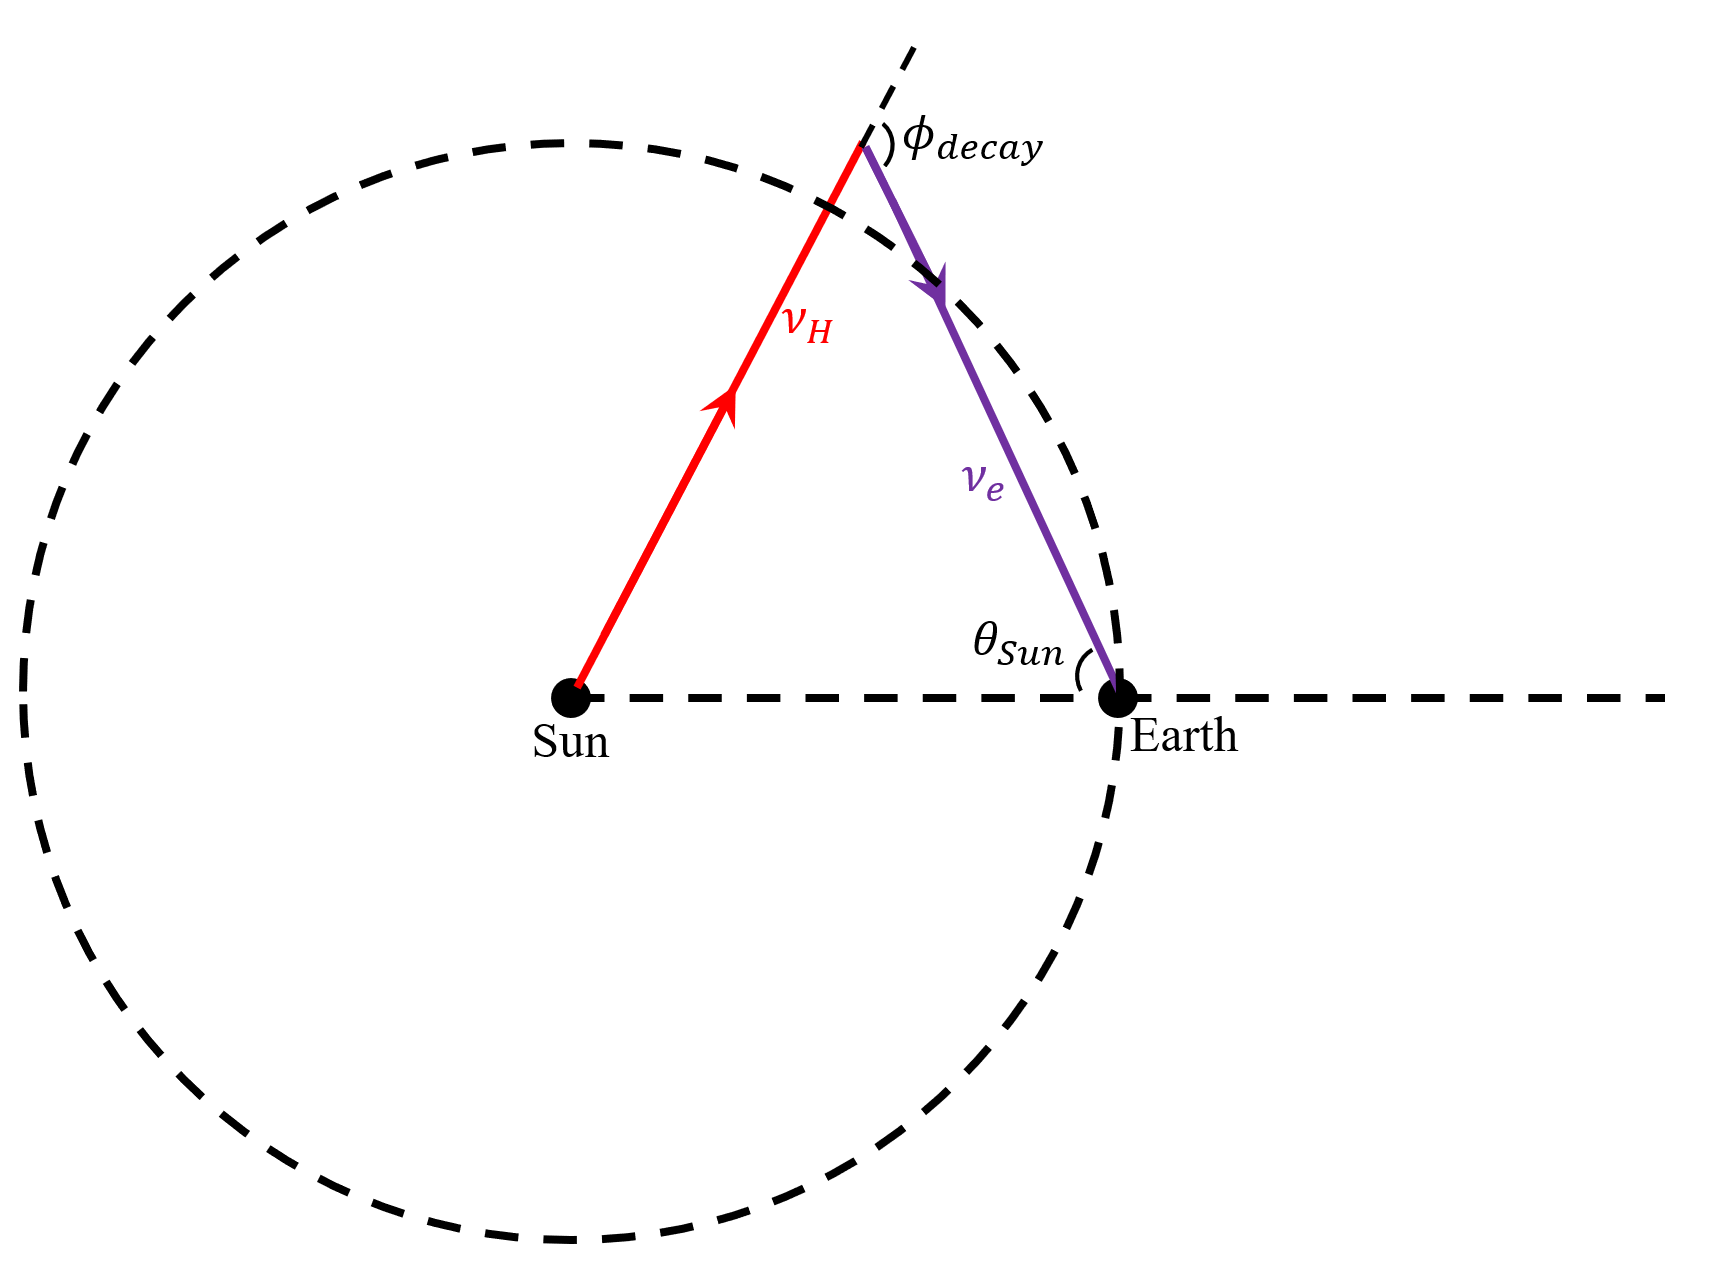
\includegraphics[width=0.45\columnwidth]{figs/decay_inflight_sketch3.png}
\caption{Definition of angles $\phi_{decay}$ (emission angle) and $\theta_{Sun}$ (solar angle) for $\nu_H$ decay in flight and then the decay product $\nu_e$ reaches the detector on earth. Different scenarios of $\nu_H$ decays are shown: $\nu_H$ decay inside earth orbit (top plot), and $\nu_H$ decay outside earth orbit (bottom plots).}
\label{fig:decay_inflight_sketch} 
\end{figure}


\begin{figure}[!htbp]
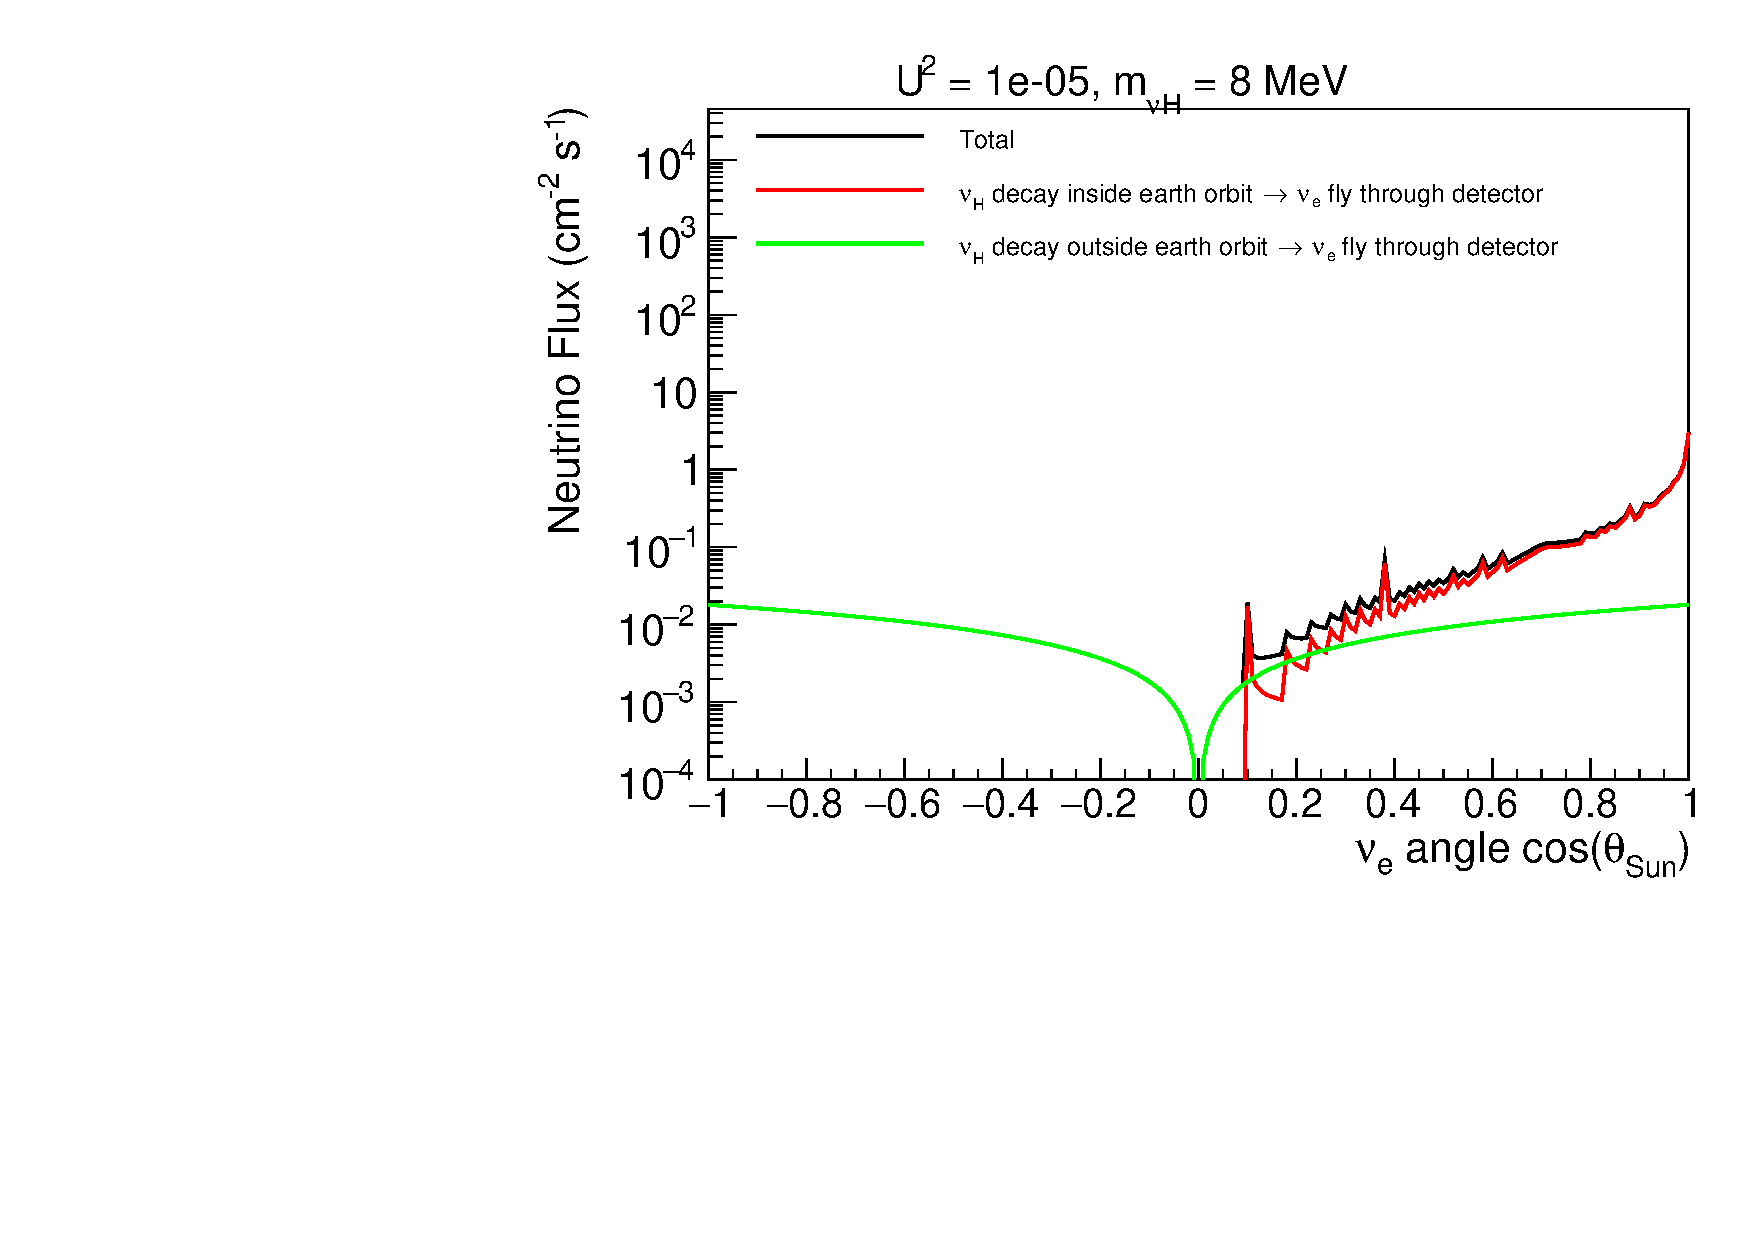
\includegraphics[width=0.99\columnwidth]{../plots/DecayInFlightNuLCosthetaSun_U1e-05_M8.0_InsideOutside_linXlogY.pdf}
\caption{Distribution solar angle $\cos(\theta_{Sun})$ of $\nu_e$'s that come from $\nu_H$ decay in flight and then reach the detector on earth. The distributions for $\nu_H$ decay inside and outside earth orbit are shown separately. The signal model shown in this plot is $m_{\nu H} = 8$ MeV and $|U_{eH}|^2 = 10^{-8}$.}
\label{fig:DecayInFlightTheta_U1em5_M8} 
\end{figure}


\begin{figure}[!htbp]
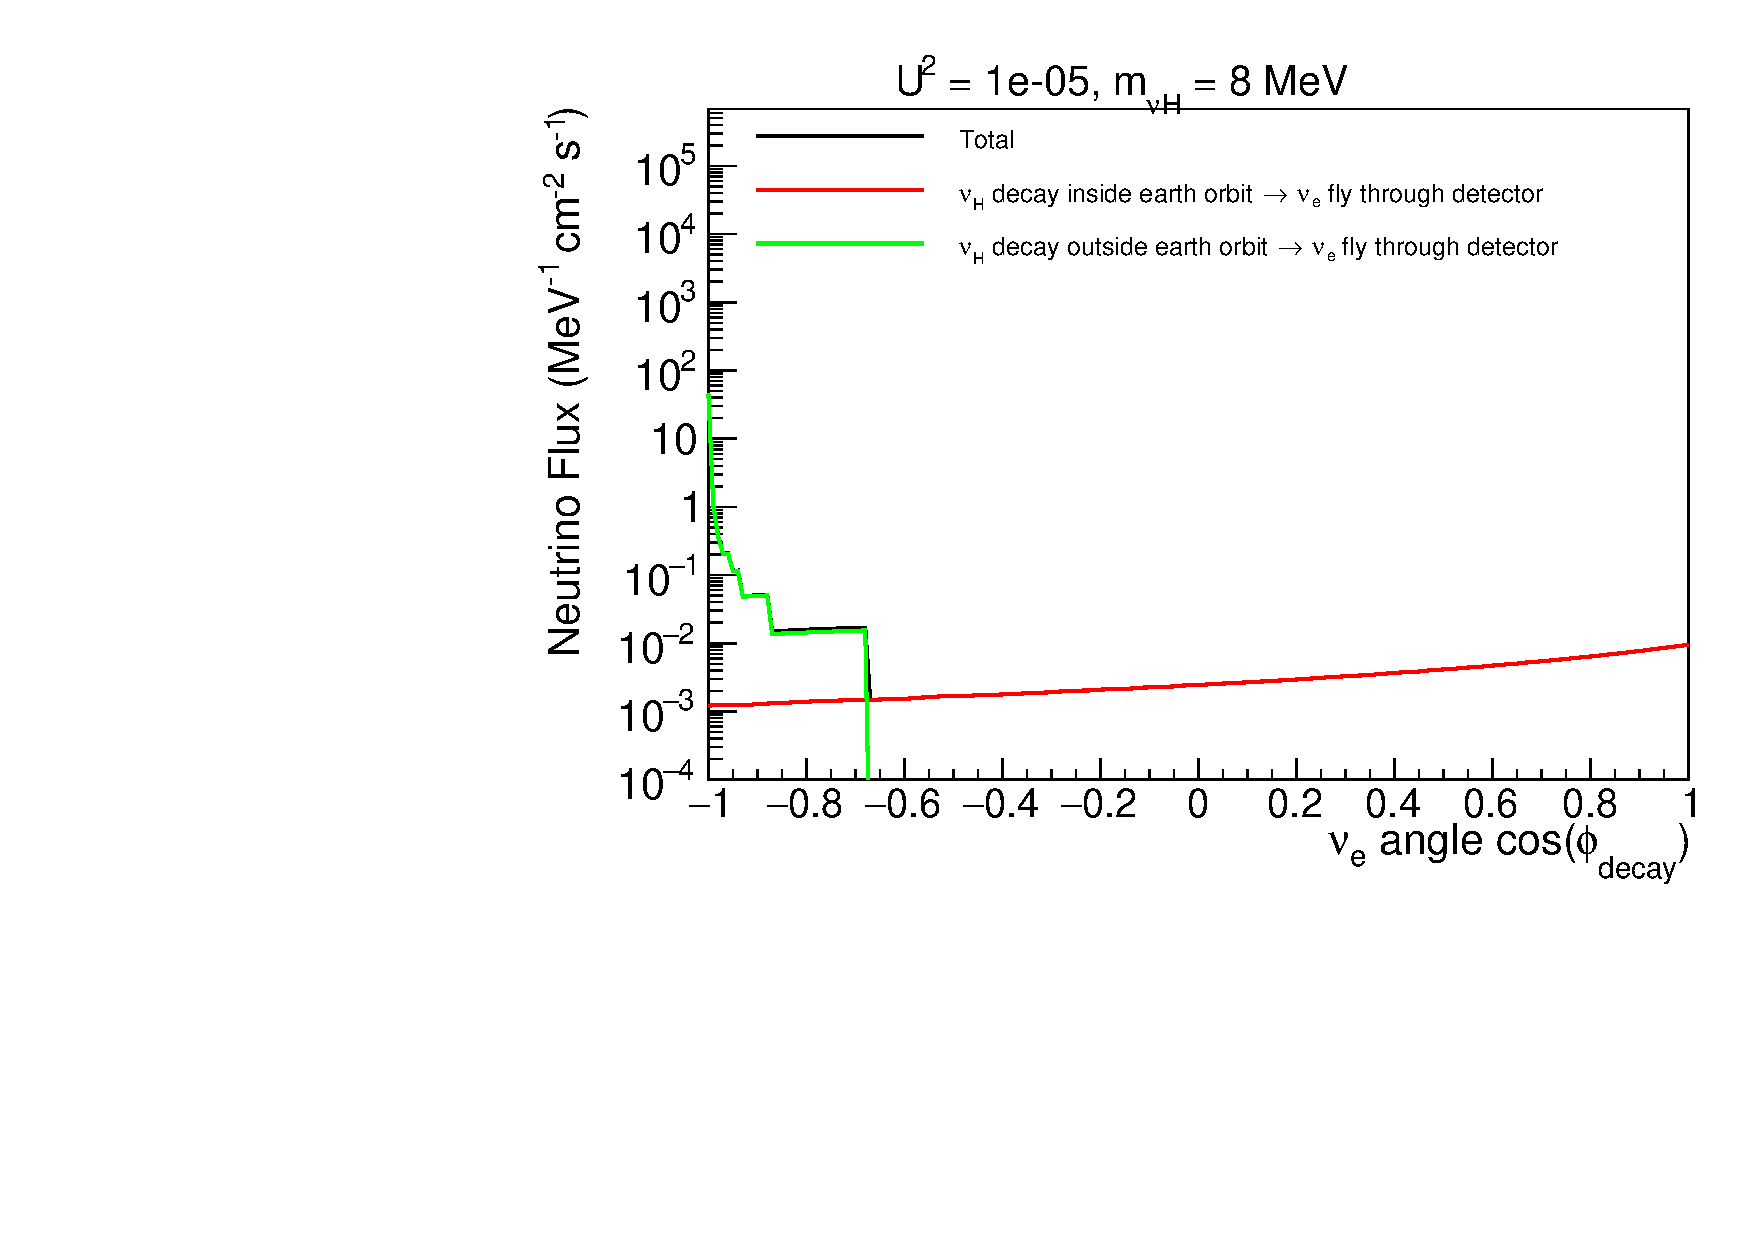
\includegraphics[width=0.99\columnwidth]{../plots/DecayInFlightNuLCosphiSun_U1e-05_M8.0_InsideOutside_linXlogY.pdf}
\caption{Distributions of emission angle $\cos(\phi_{decay})$ of $\nu_e$'s that come from $\nu_H$ decay in flight and then reach the detector on earth. The distributions for $\nu_H$ decay inside and outside earth orbit are shown separately. The signal model shown in this plot is $m_{\nu H} = 8$ MeV and $|U_{eH}|^2 = 10^{-5}$.}
\label{fig:DecayInFlightPhi_U1em5_M8} 
\end{figure}

\begin{figure}[!htbp]
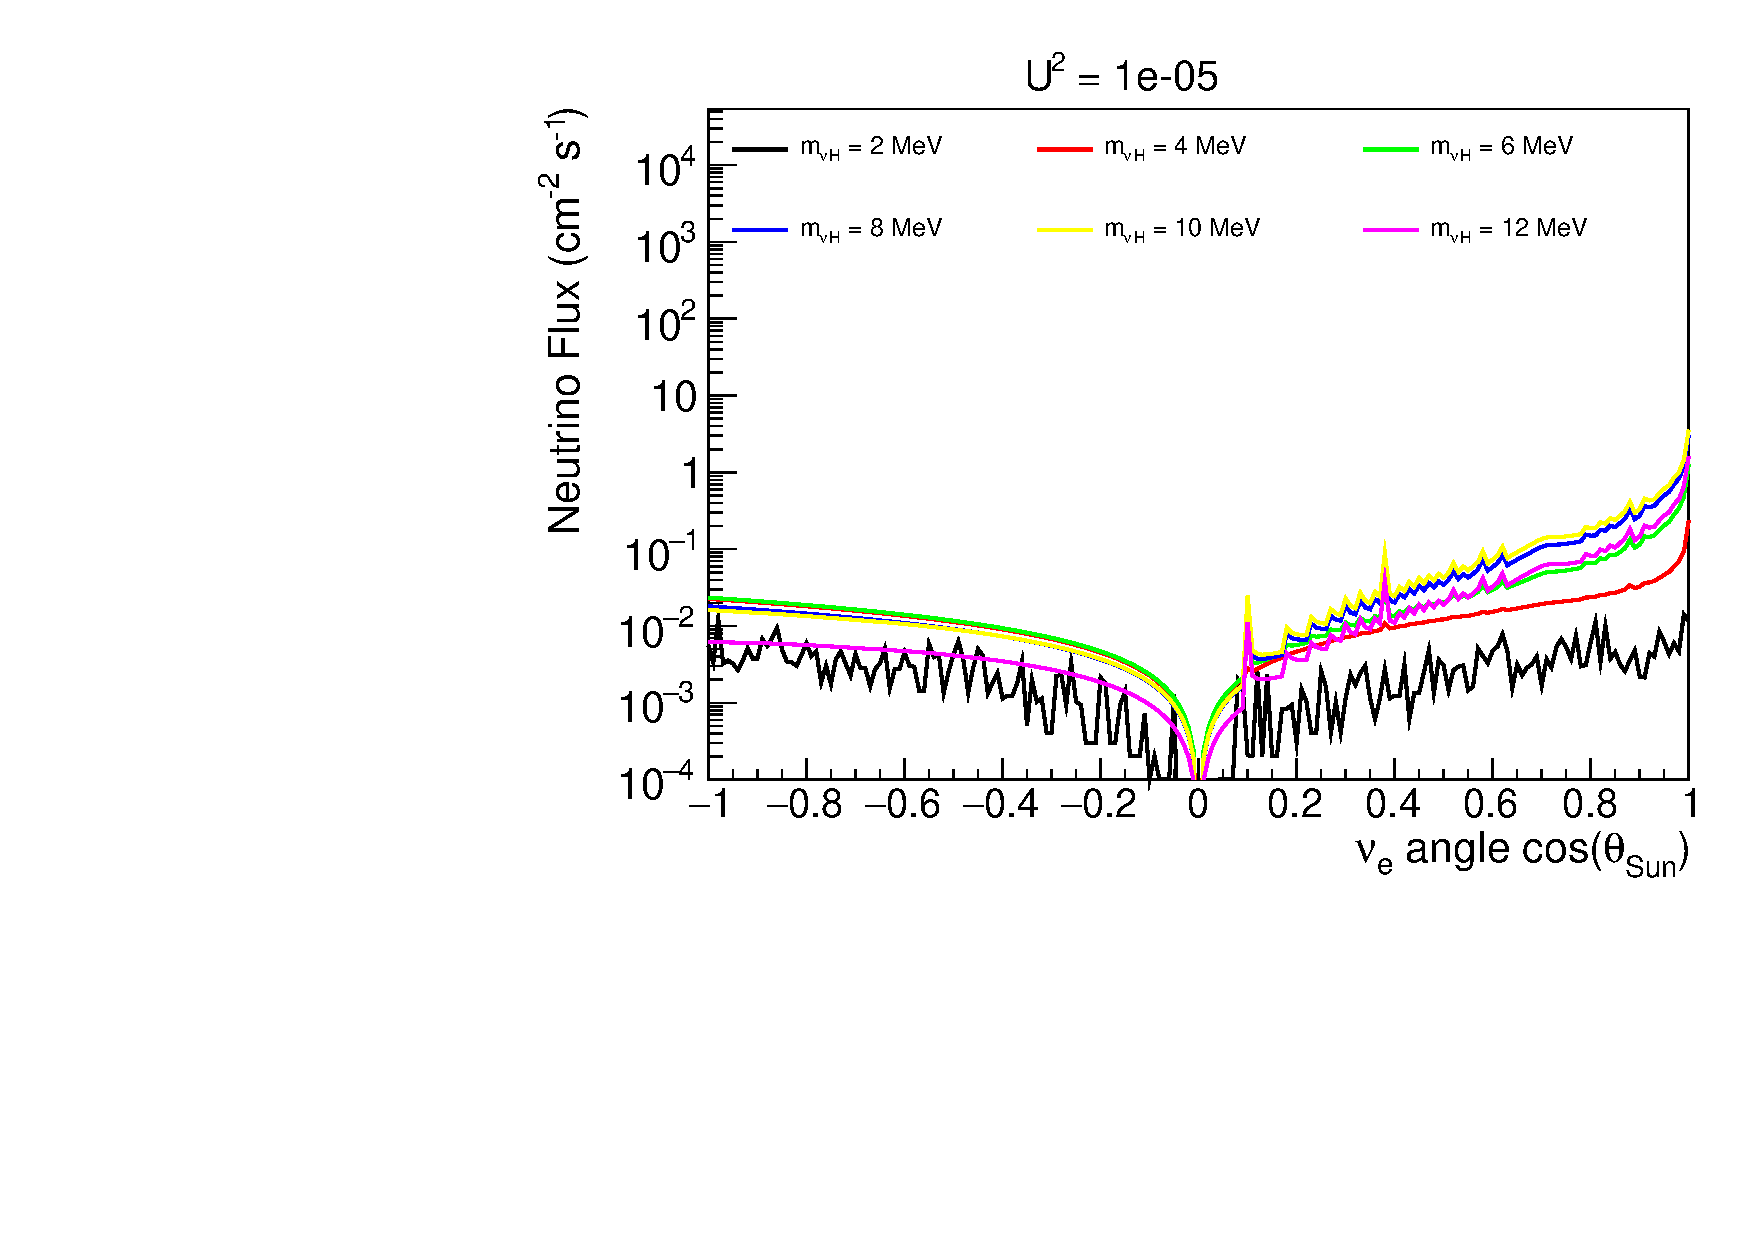
\includegraphics[width=0.99\columnwidth]{../plots/DecayInFlightNuLCosthetaSun_U1e-05_AllMass_linXlogY.pdf}
\caption{Distributions of solar angle $\cos(\theta_{Sun})$ of $\nu_e$'s that come from $\nu_H$ decay in flight and then reach the detector on earth. Different curves are for different $\nu_H$ masses $m_{\nu H}$, and the mixing angle $|U_{eH}|^2 = 10^{-5}$.}
\label{fig:DecayInFlightTheta_U1em5_AllMass}
\end{figure}

\begin{figure}[!htbp]
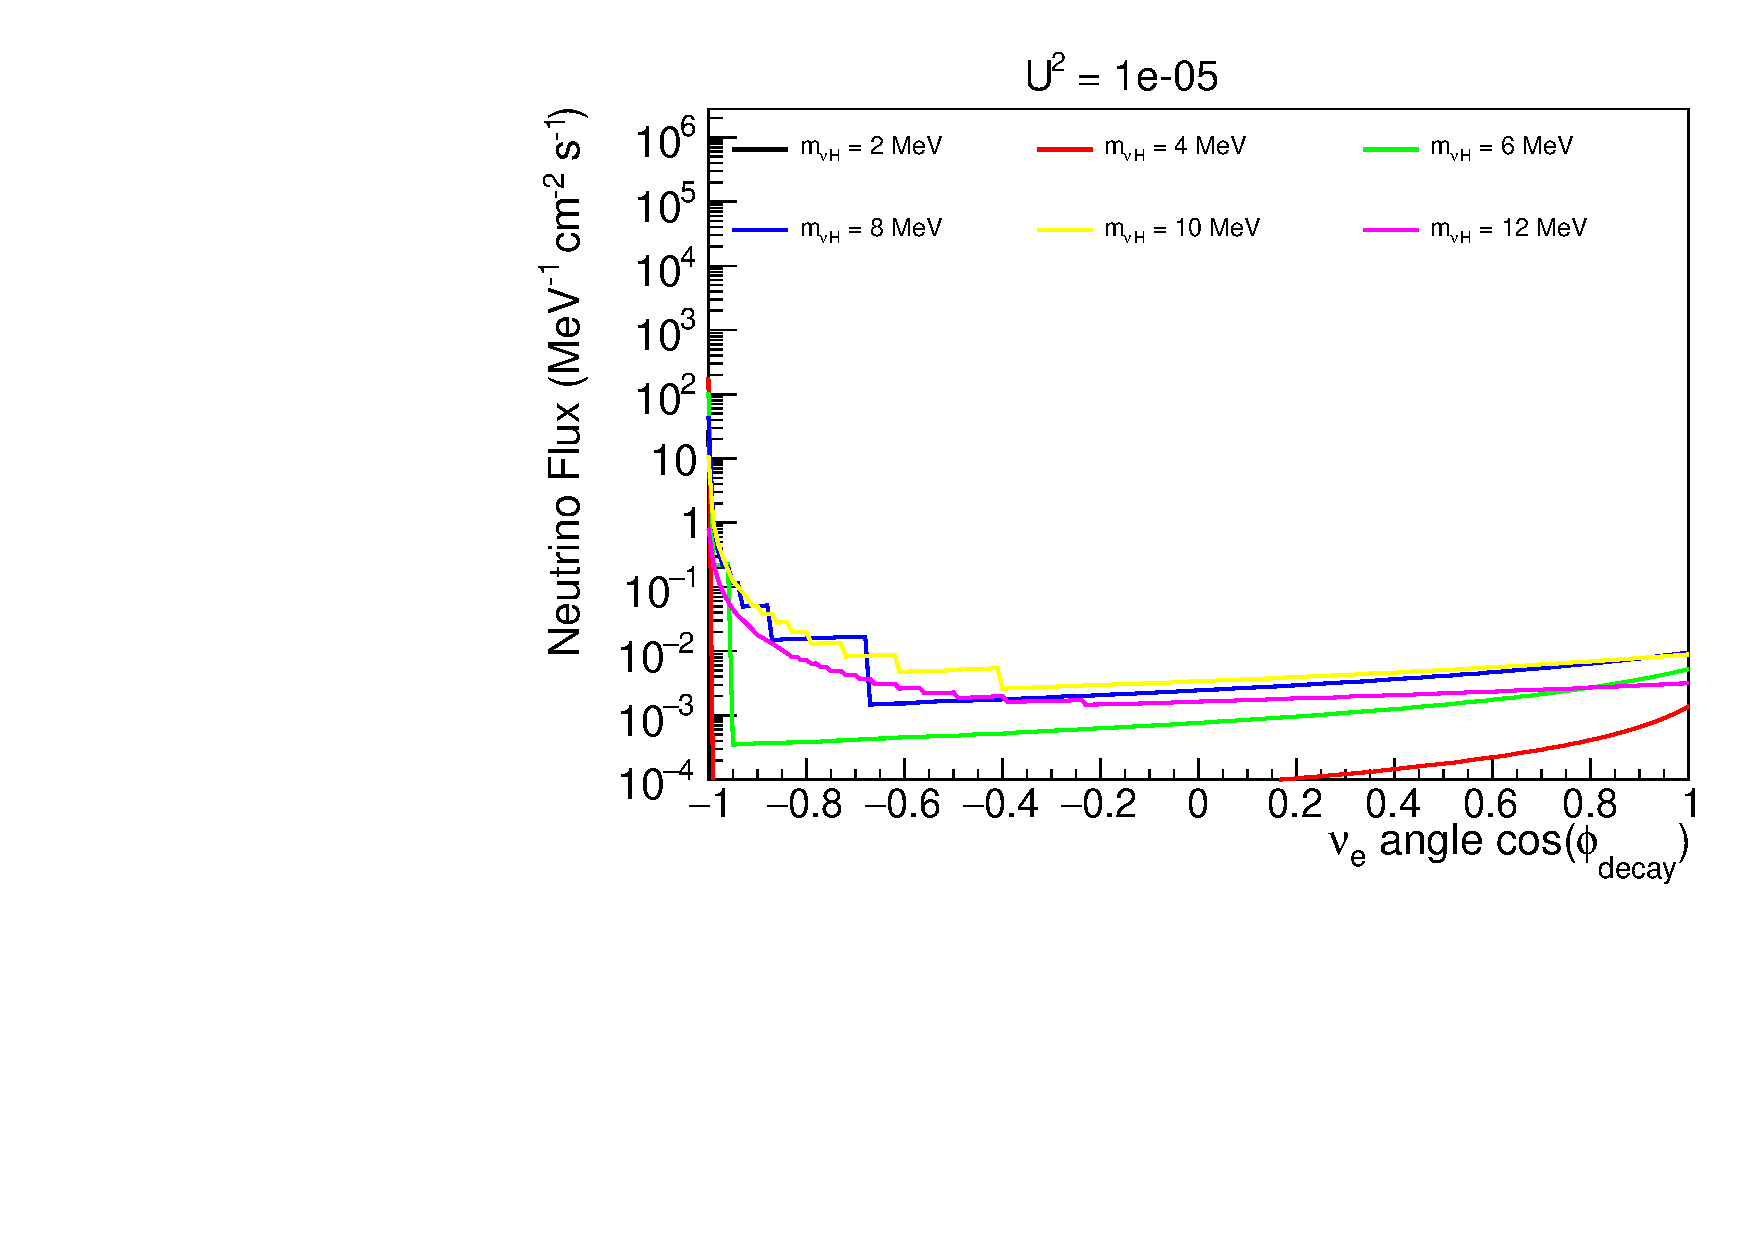
\includegraphics[width=0.99\columnwidth]{../plots/DecayInFlightNuLCosphiSun_U1e-05_AllMass_linXlogY.pdf}
\caption{Distributions of emission angle $\cos(\phi_{decay})$ of $\nu_e$'s that come from $\nu_H$ decay in flight and then reach the detector on earth. Different curves are for different $\nu_H$ masses $m_{\nu H}$, and the mixing angle $|U_{eH}|^2 = 10^{-5}$.}
\label{fig:DecayInFlightPhi_U1em5_AllMass}
\end{figure}


\begin{figure}[!htbp]
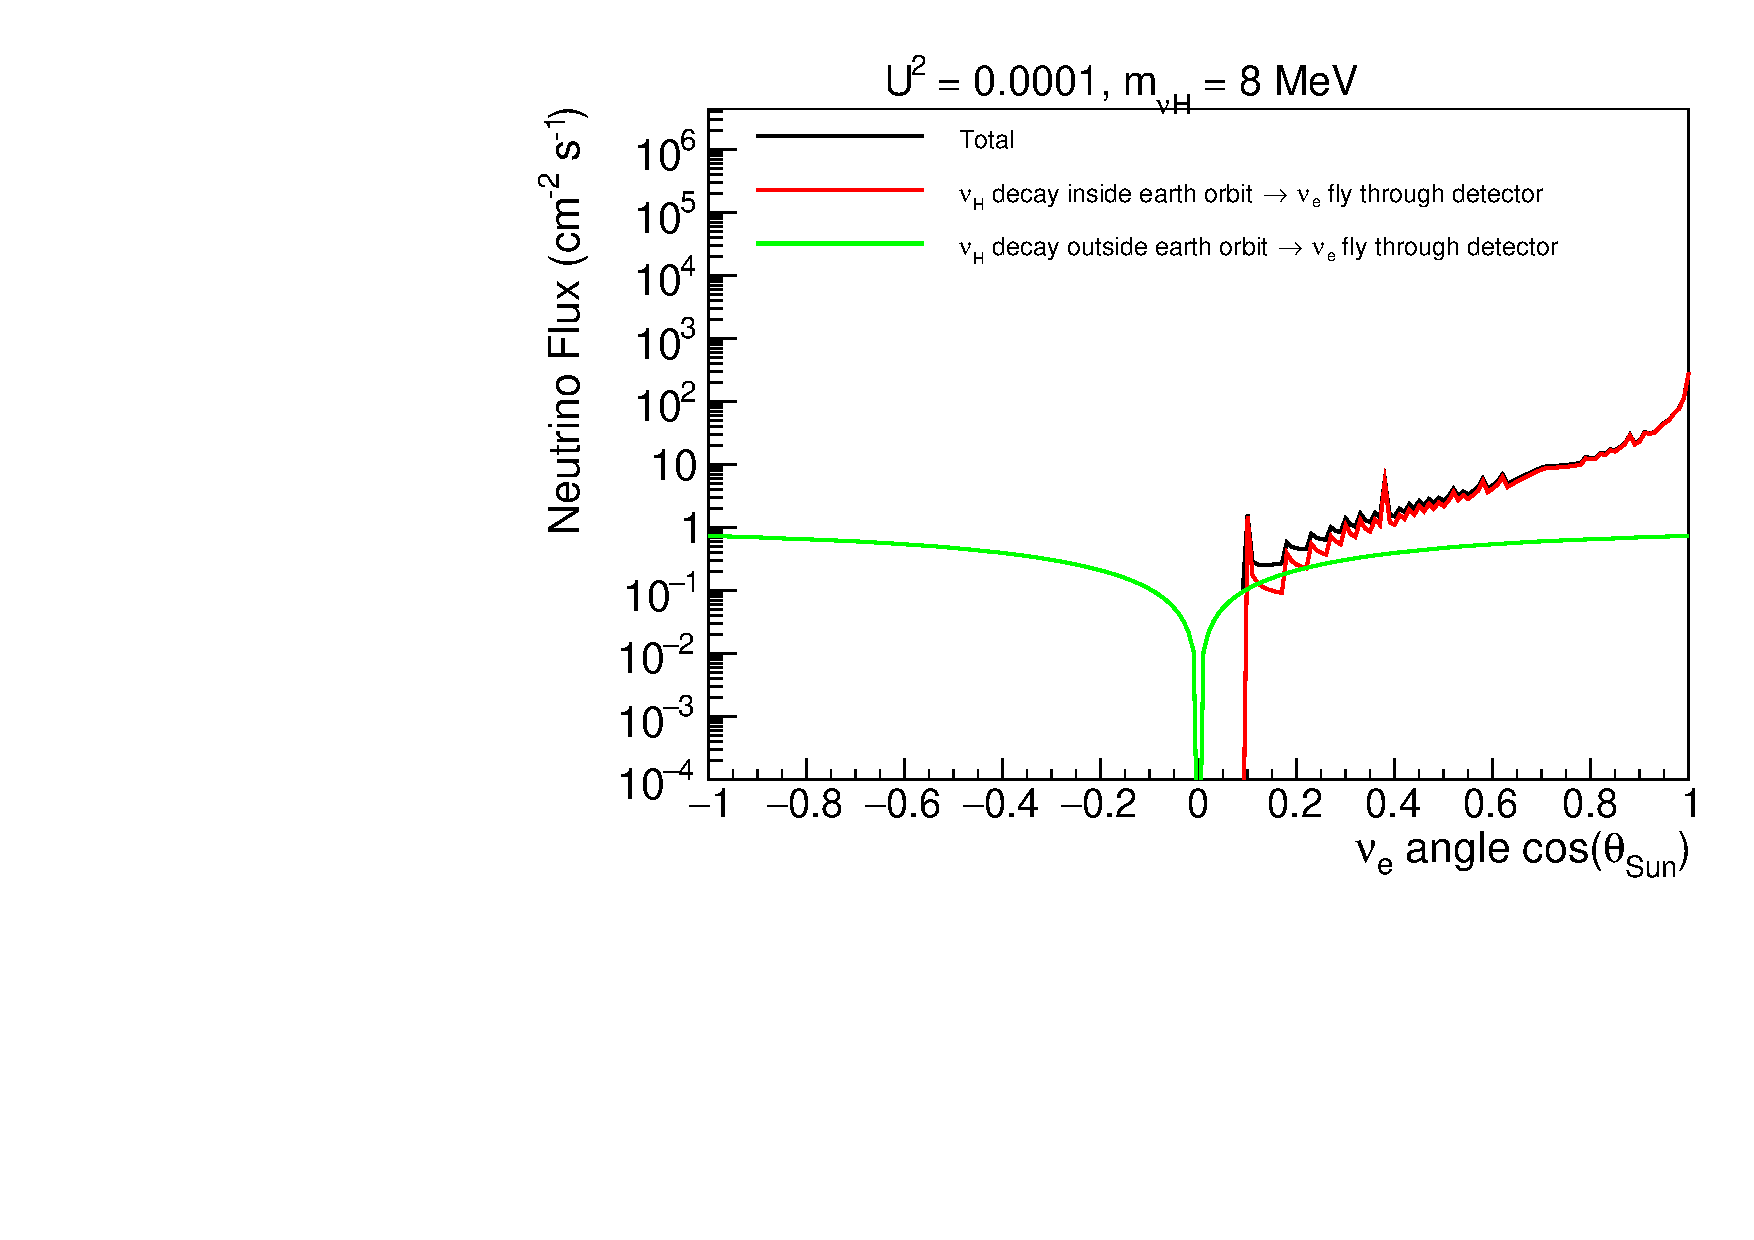
\includegraphics[width=0.99\columnwidth]{../plots/DecayInFlightNuLCosthetaSun_U0.0001_M8.0_InsideOutside_linXlogY.pdf}
\caption{Distribution solar angle $\cos(\theta_{Sun})$ of $\nu_e$'s that come from $\nu_H$ decay in flight and then reach the detector on earth. The distributions for $\nu_H$ decay inside and outside earth orbit are shown separately. The signal model shown in this plot is $m_{\nu H} = 8$ MeV and $|U_{eH}|^2 = 10^{-4}$.}
\label{fig:DecayInFlightTheta_U0.0001_M8} 
\end{figure}


\begin{figure}[!htbp]
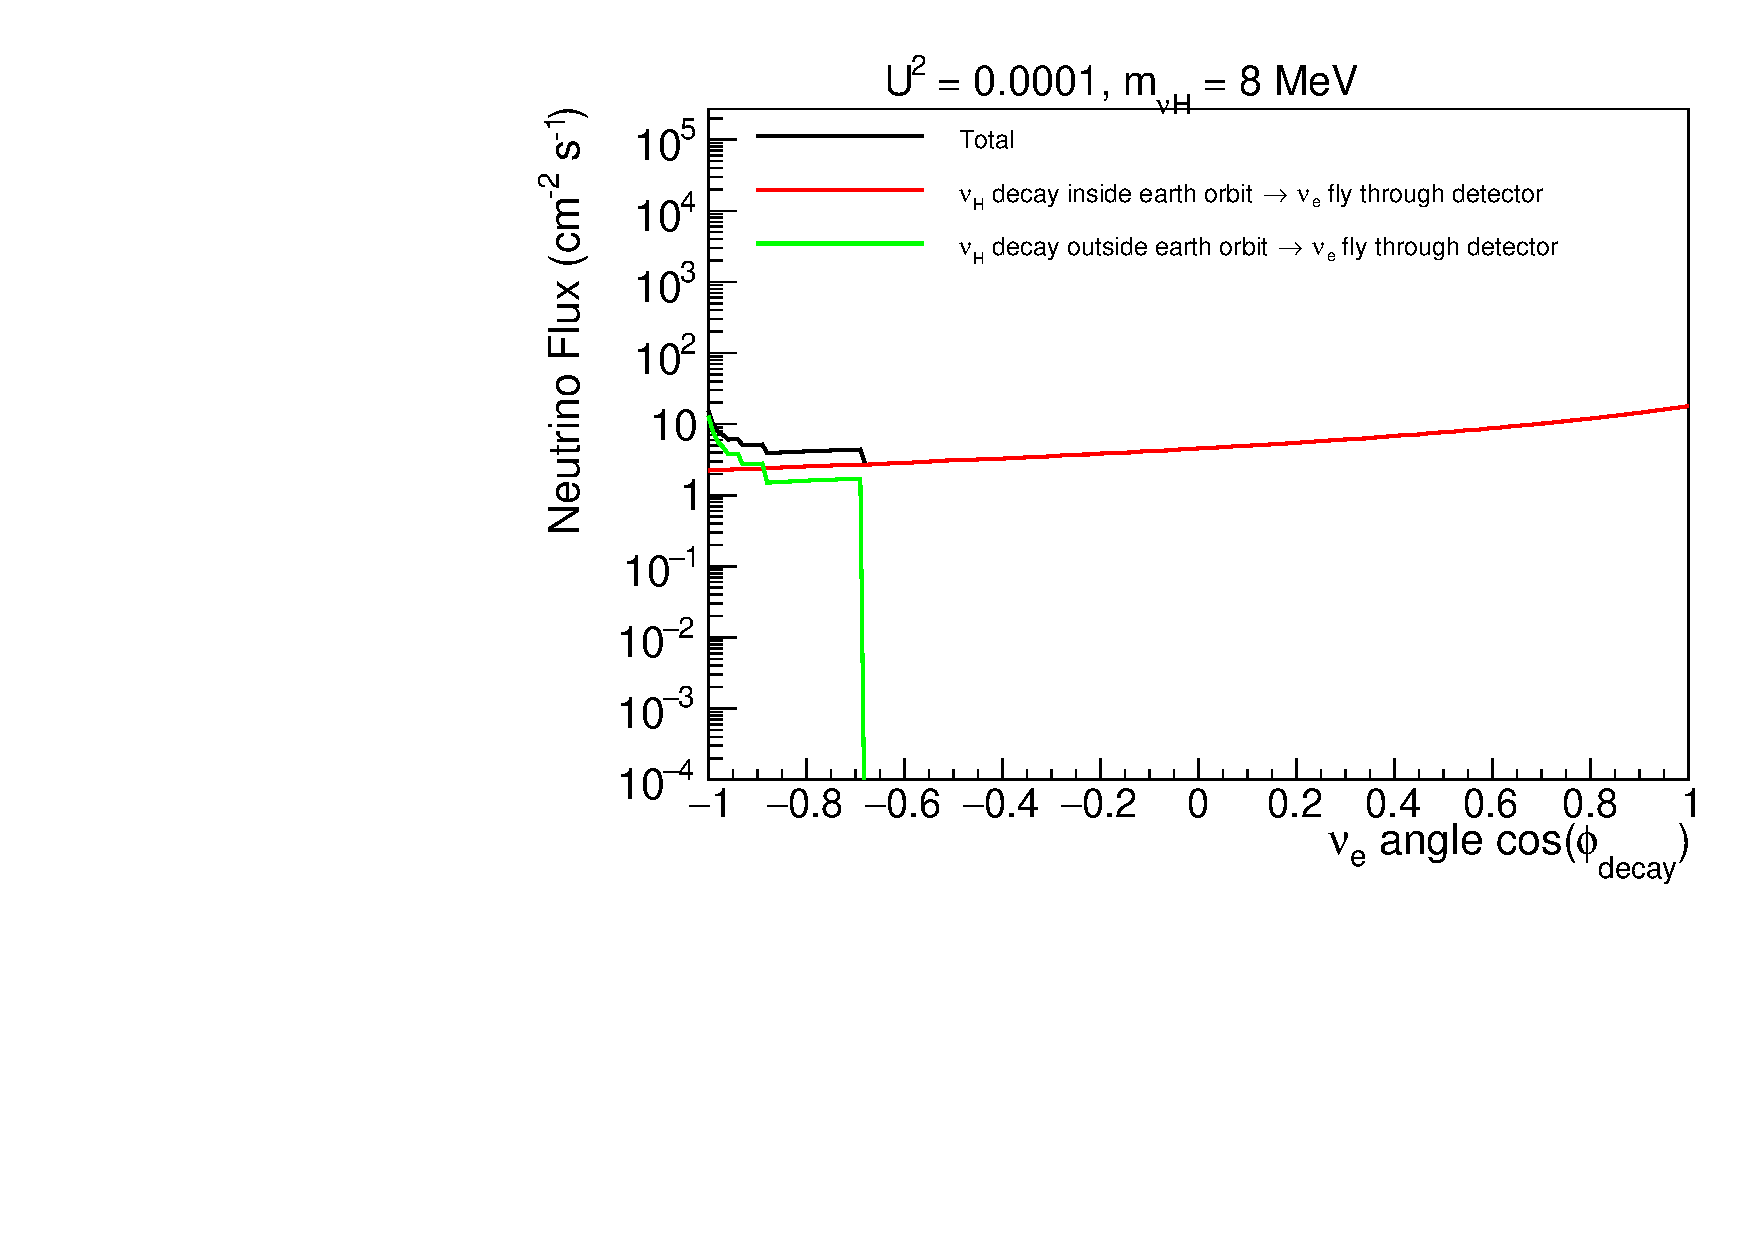
\includegraphics[width=0.99\columnwidth]{../plots/DecayInFlightNuLCosphiSun_U0.0001_M8.0_InsideOutside_linXlogY.pdf}
\caption{Distributions of emission angle $\cos(\phi_{decay})$ of $\nu_e$'s that come from $\nu_H$ decay in flight and then reach the detector on earth. The distributions for $\nu_H$ decay inside and outside earth orbit are shown separately. The signal model shown in this plot is $m_{\nu H} = 8$ MeV and $|U_{eH}|^2 = 10^{-4}$.}
\label{fig:DecayInFlightPhi_U0.0001_M8} 
\end{figure}

\begin{figure}[!htbp]
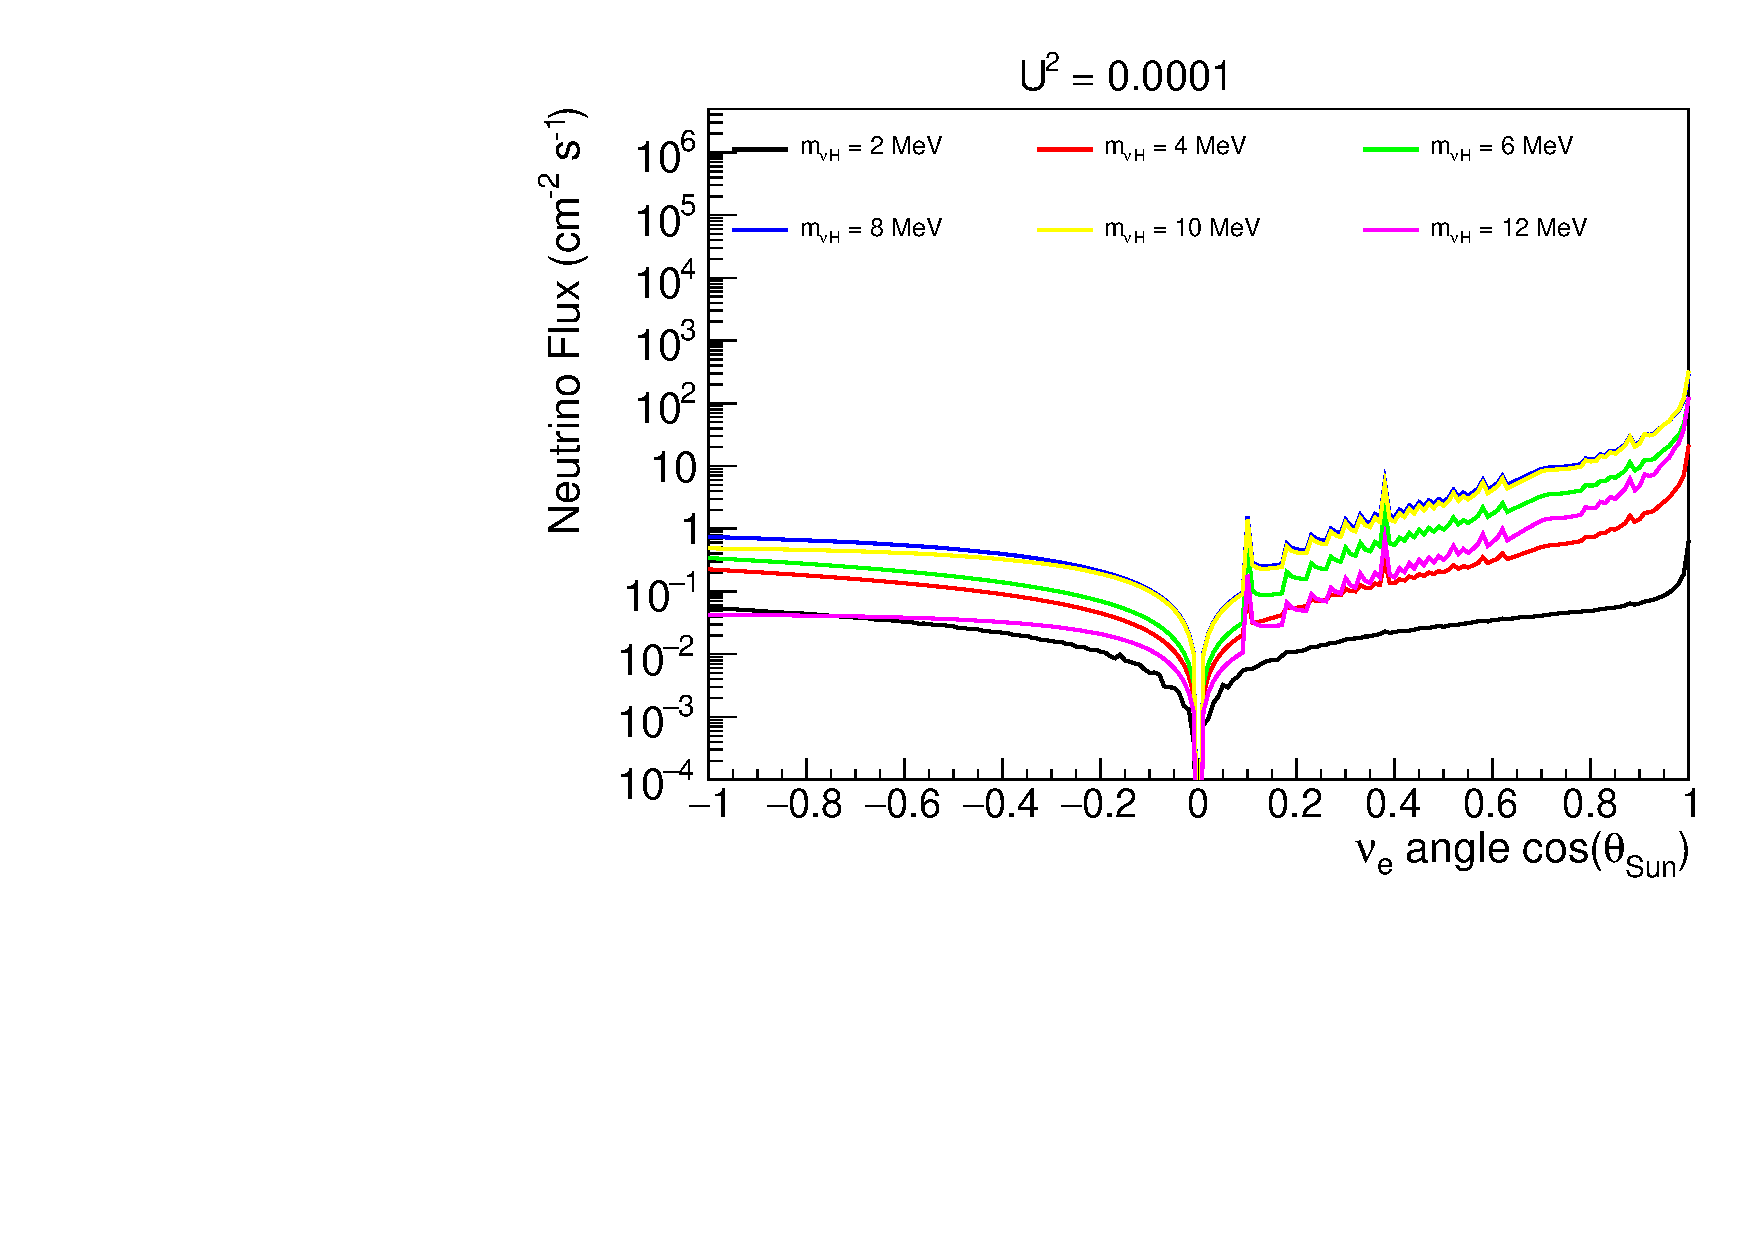
\includegraphics[width=0.99\columnwidth]{../plots/DecayInFlightNuLCosthetaSun_U0.0001_AllMass_linXlogY.pdf}
\caption{Distributions of solar angle $\cos(\theta_{Sun})$ of $\nu_e$'s that come from $\nu_H$ decay in flight and then reach the detector on earth. Different curves are for different $\nu_H$ masses $m_{\nu H}$, and the mixing angle $|U_{eH}|^2 = 10^{-4}$.}
\label{fig:DecayInFlightTheta_U1em4_AllMass}
\end{figure}

\begin{figure}[!htbp]
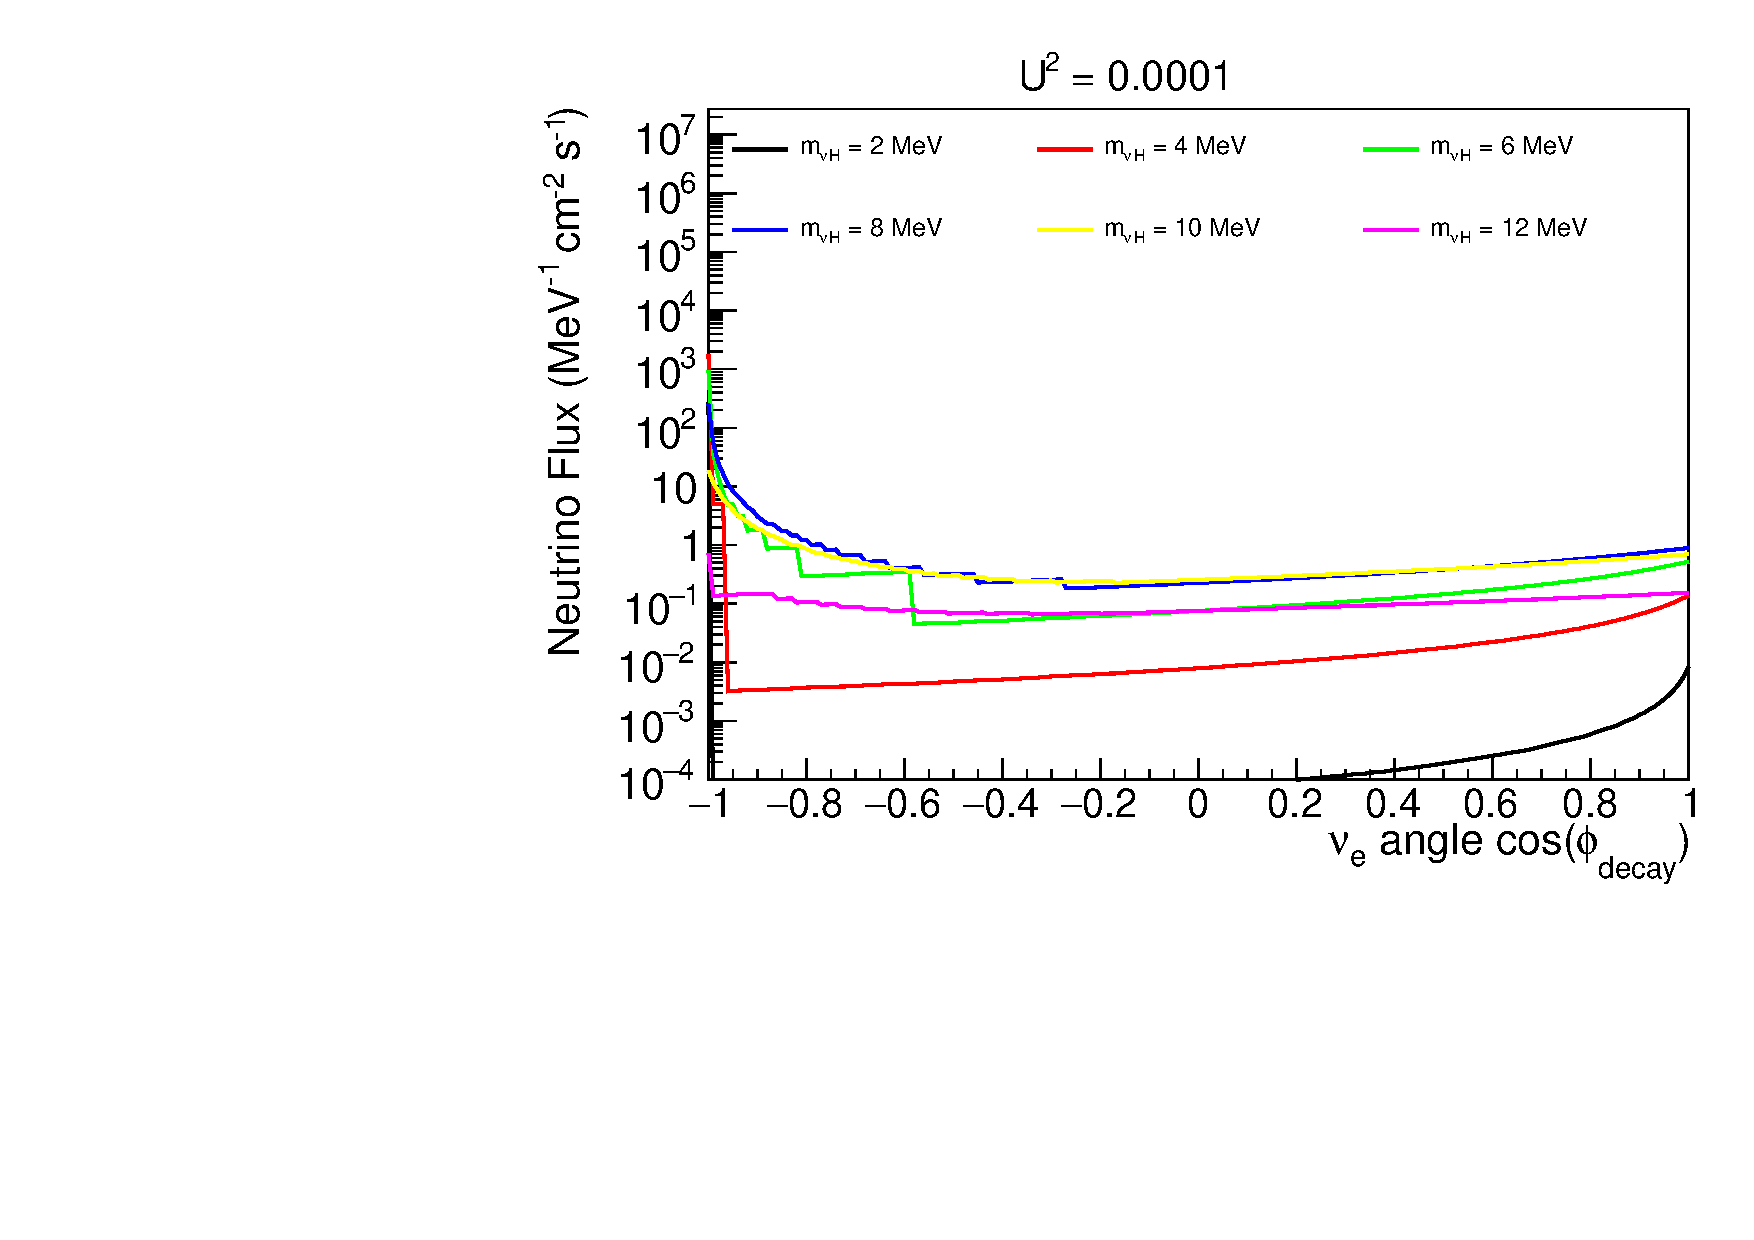
\includegraphics[width=0.99\columnwidth]{../plots/DecayInFlightNuLCosphiSun_U0.0001_AllMass_linXlogY.pdf}
\caption{Distributions of emission angle $\cos(\phi_{decay})$ of $\nu_e$'s that come from $\nu_H$ decay in flight and then reach the detector on earth. Different curves are for different $\nu_H$ masses $m_{\nu H}$, and the mixing angle $|U_{eH}|^2 = 10^{-4}$.}
\label{fig:DecayInFlightPhi_U1em4_AllMass}
\end{figure}


\begin{figure}[!htbp]
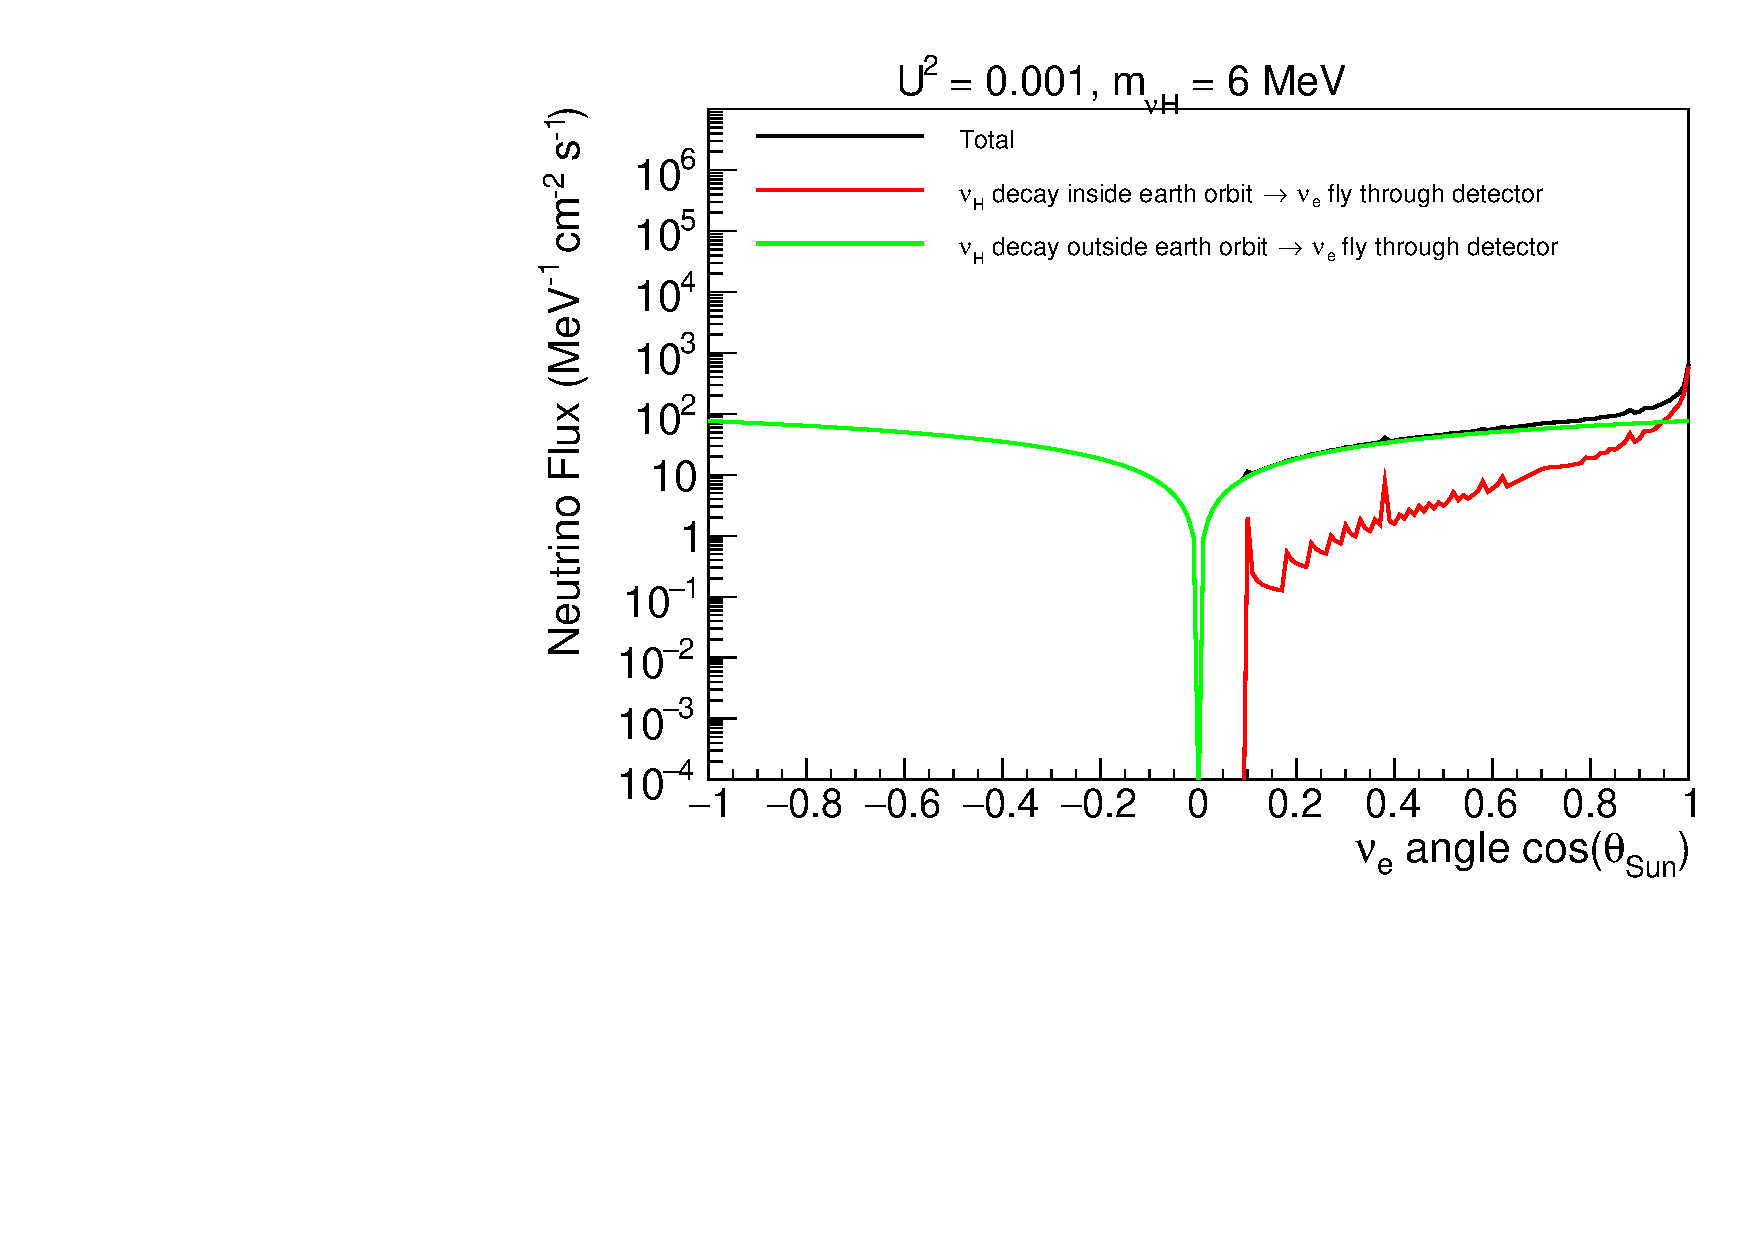
\includegraphics[width=0.99\columnwidth]{../plots/DecayInFlightNuLCosthetaSun_U0.001_M6.0_InsideOutside_linXlogY.pdf}
\caption{Distribution solar angle $\cos(\theta_{Sun})$ of $\nu_e$'s that come from $\nu_H$ decay in flight and then reach the detector on earth. The distributions for $\nu_H$ decay inside and outside earth orbit are shown separately. The signal model shown in this plot is $m_{\nu H} = 6$ MeV and $|U_{eH}|^2 = 10^{-3}$.}
\label{fig:DecayInFlightTheta_U0.001_M6} 
\end{figure}


\begin{figure}[!htbp]
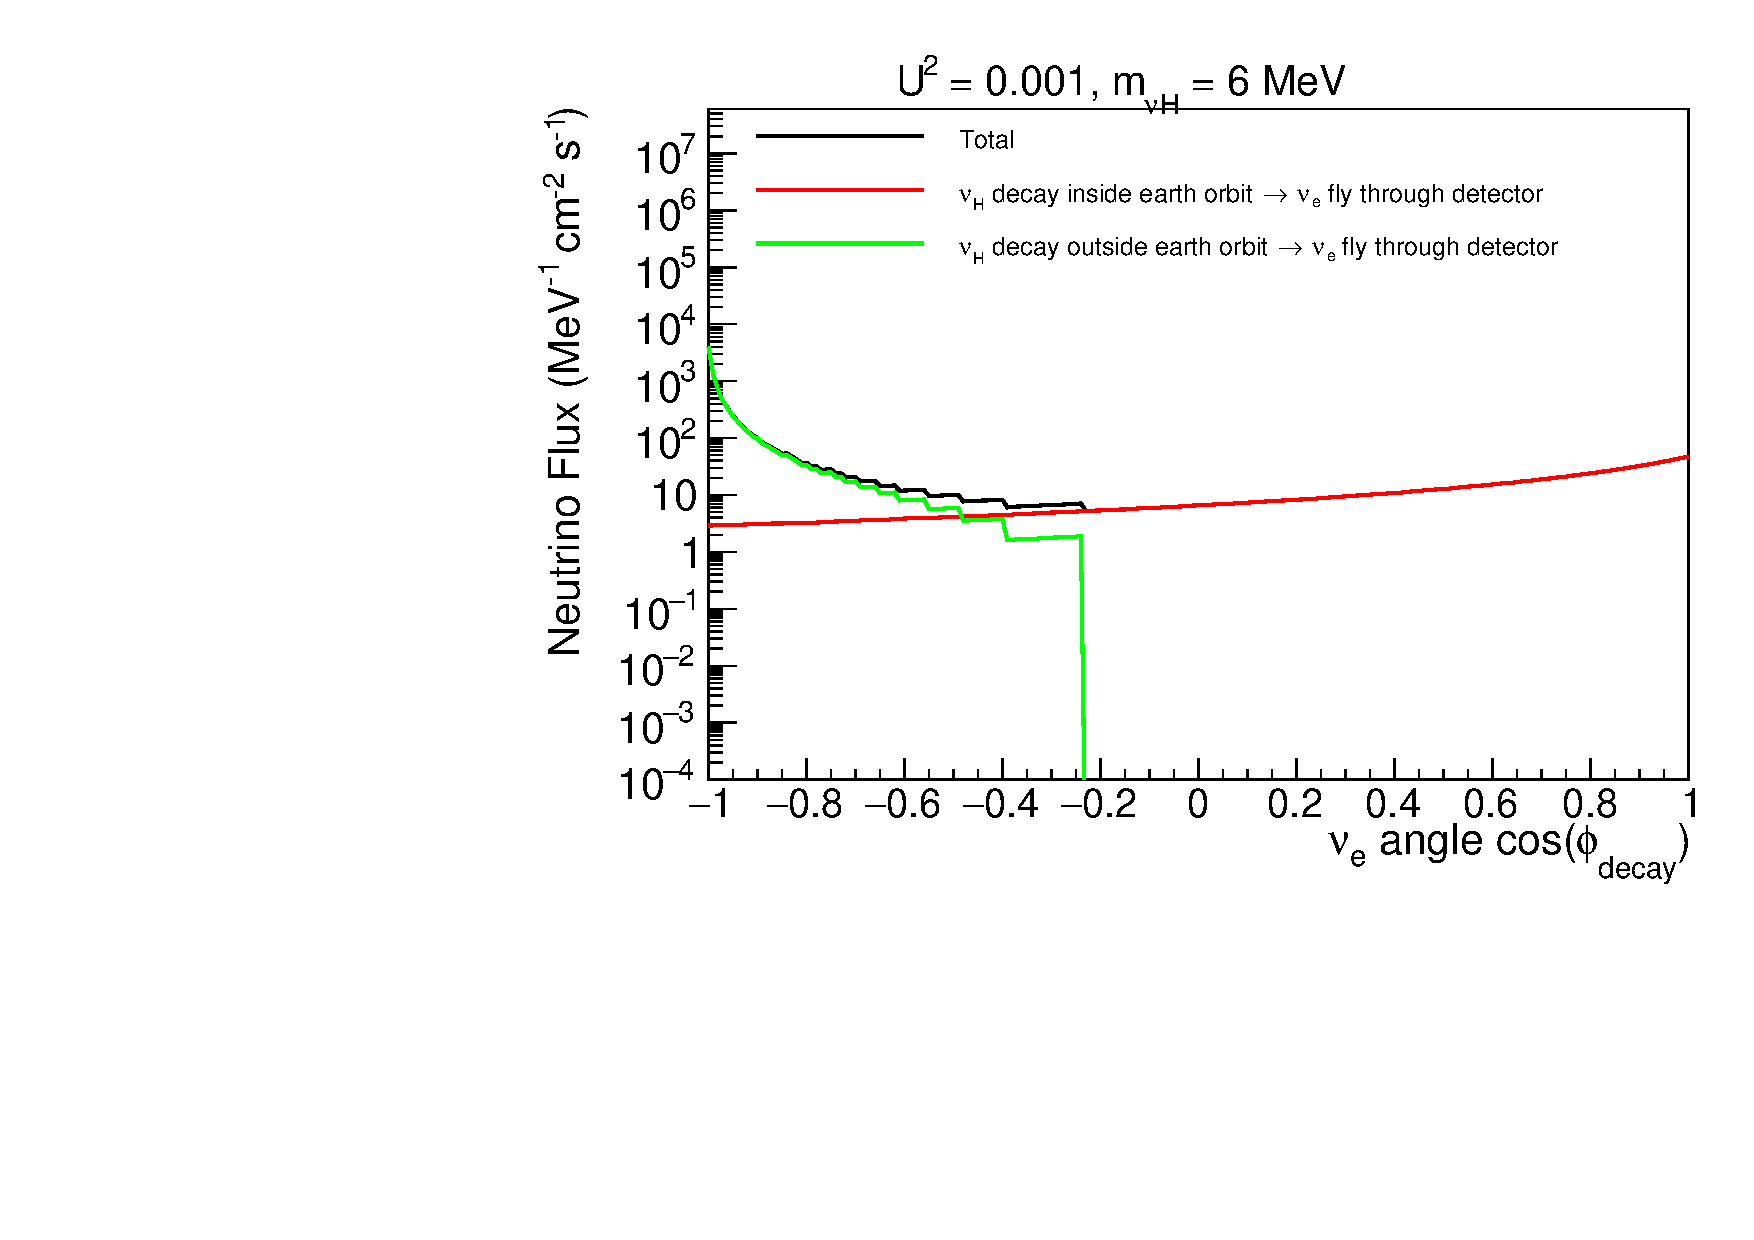
\includegraphics[width=0.99\columnwidth]{../plots/DecayInFlightNuLCosphiSun_U0.001_M6.0_InsideOutside_linXlogY.pdf}
\caption{Distributions of emission angle $\cos(\phi_{decay})$ of $\nu_e$'s that come from $\nu_H$ decay in flight and then reach the detector on earth. The distributions for $\nu_H$ decay inside and outside earth orbit are shown separately. The signal model shown in this plot is $m_{\nu H} = 6$ MeV and $|U_{eH}|^2 = 10^{-3}$.}
\label{fig:DecayInFlightPhi_U0.001_M6} 
\end{figure}


\begin{figure}[!htbp]
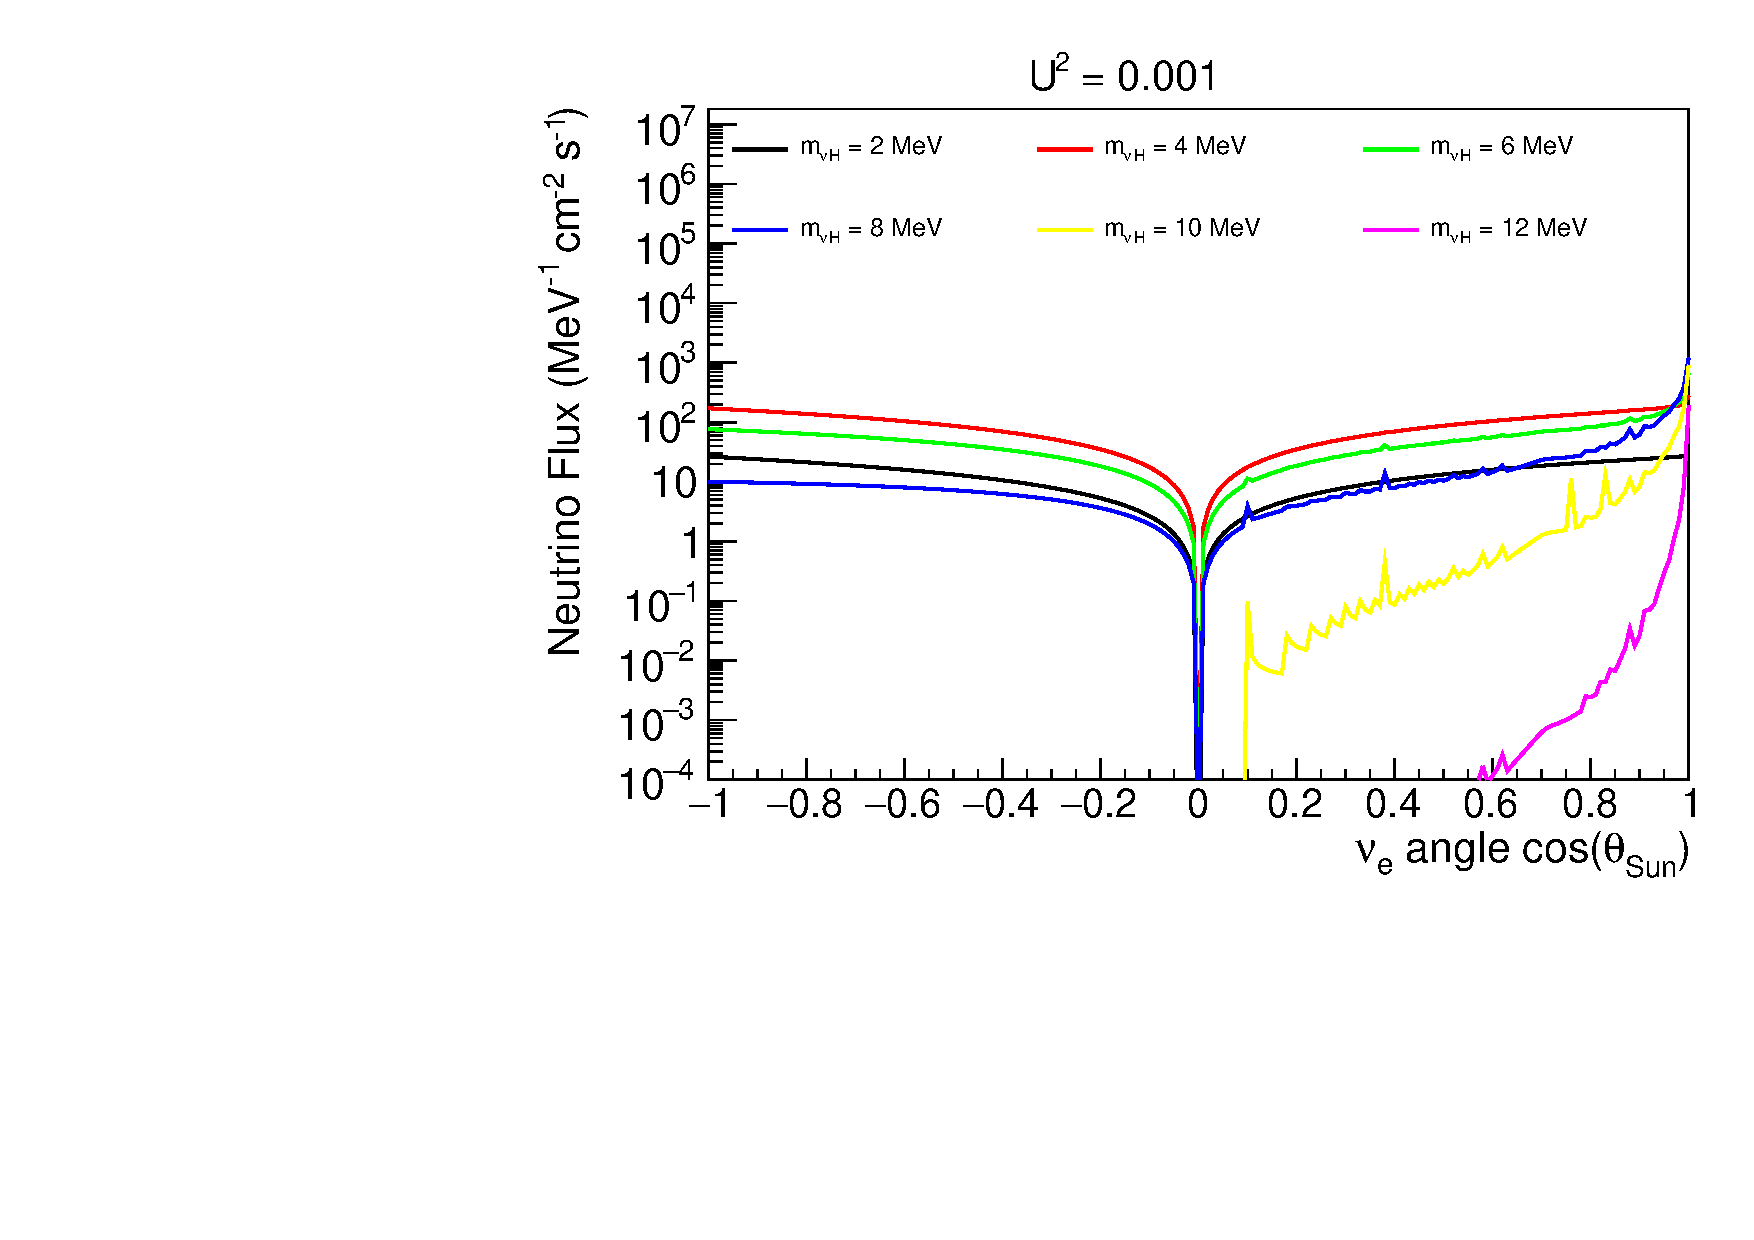
\includegraphics[width=0.99\columnwidth]{../plots/DecayInFlightNuLCosthetaSun_U0.001_AllMass_linXlogY.pdf}
\caption{Distributions of solar angle $\cos(\theta_{Sun})$ of $\nu_e$'s that come from $\nu_H$ decay in flight and then reach the detector on earth. Different curves are for different $\nu_H$ masses $m_{\nu H}$, and the mixing angle $|U_{eH}|^2 = 10^{-3}$.}
\label{fig:DecayInFlightTheta_U1em3_AllMass}
\end{figure}

\begin{figure}[!htbp]
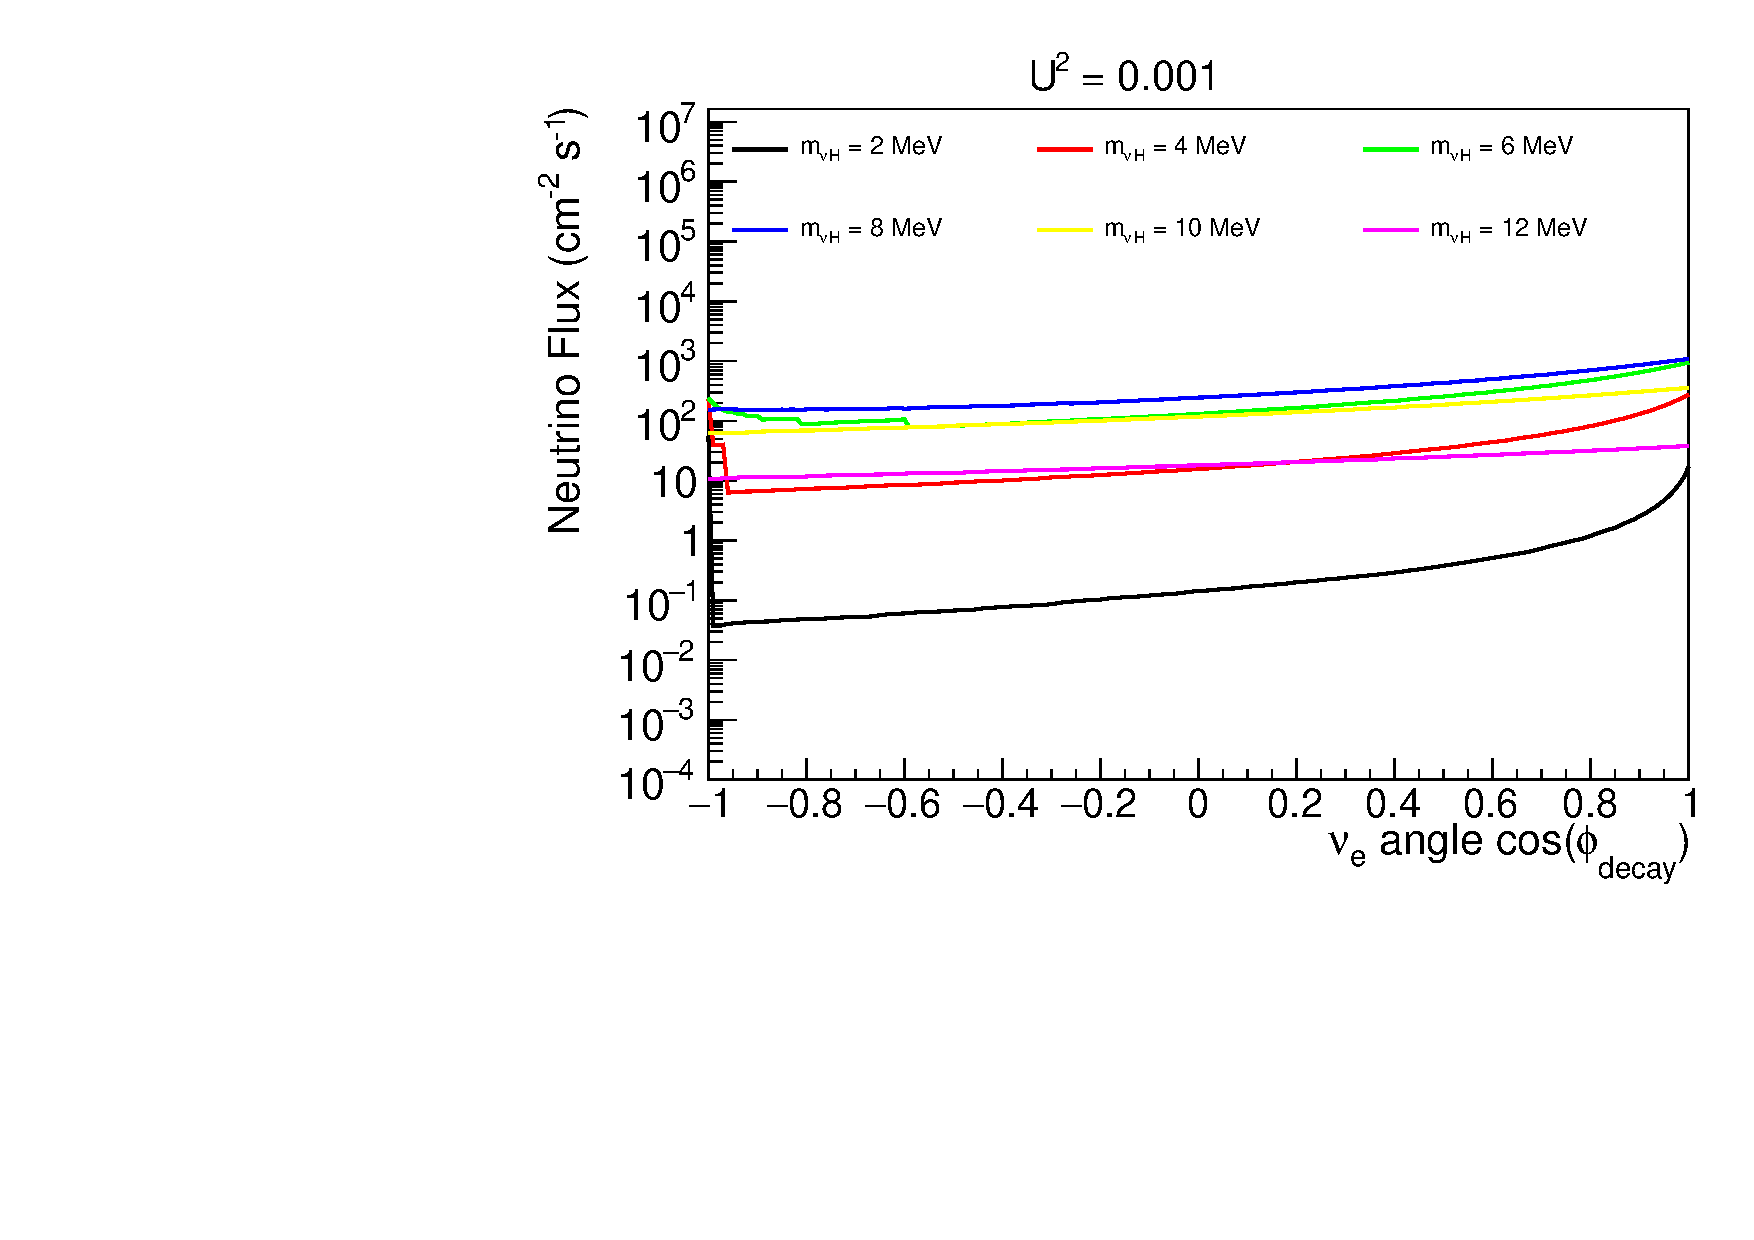
\includegraphics[width=0.99\columnwidth]{../plots/DecayInFlightNuLCosphiSun_U0.001_AllMass_linXlogY.pdf}
\caption{Distributions of emission angle $\cos(\phi_{decay})$ of $\nu_e$'s that come from $\nu_H$ decay in flight and then reach the detector on earth. Different curves are for different $\nu_H$ masses $m_{\nu H}$, and the mixing angle $|U_{eH}|^2 = 10^{-3}$.}
\label{fig:DecayInFlightPhi_U1em3_AllMass}
\end{figure}

\begin{figure}[!htbp]
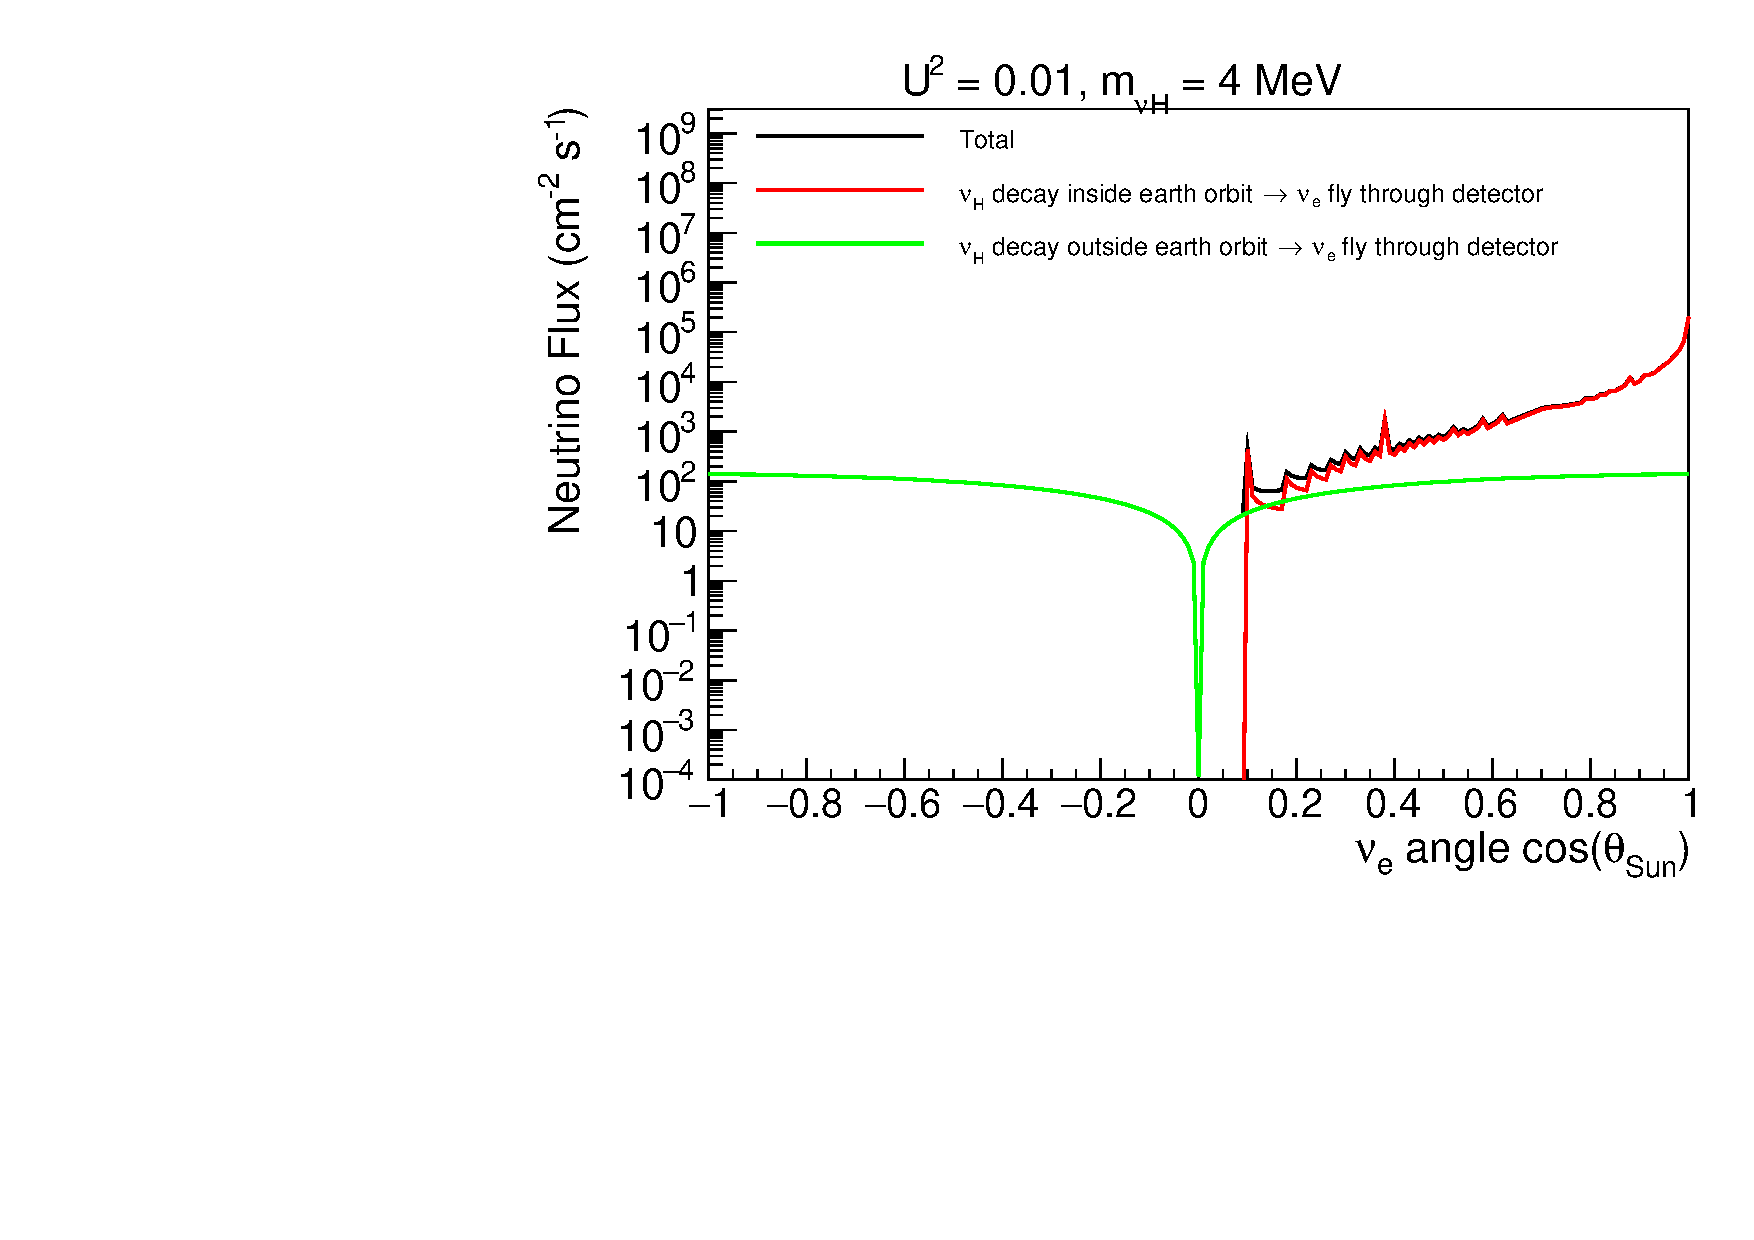
\includegraphics[width=0.99\columnwidth]{../plots/DecayInFlightNuLCosthetaSun_U0.01_M4.0_InsideOutside_linXlogY.pdf}
\caption{Distribution solar angle $\cos(\theta_{Sun})$ of $\nu_e$'s that come from $\nu_H$ decay in flight and then reach the detector on earth. The distributions for $\nu_H$ decay inside and outside earth orbit are shown separately. The signal model shown in this plot is $m_{\nu H} = 4$ MeV and $|U_{eH}|^2 = 10^{-2}$.}
\label{fig:DecayInFlightTheta_U0.01_M4} 
\end{figure}


\begin{figure}[!htbp]
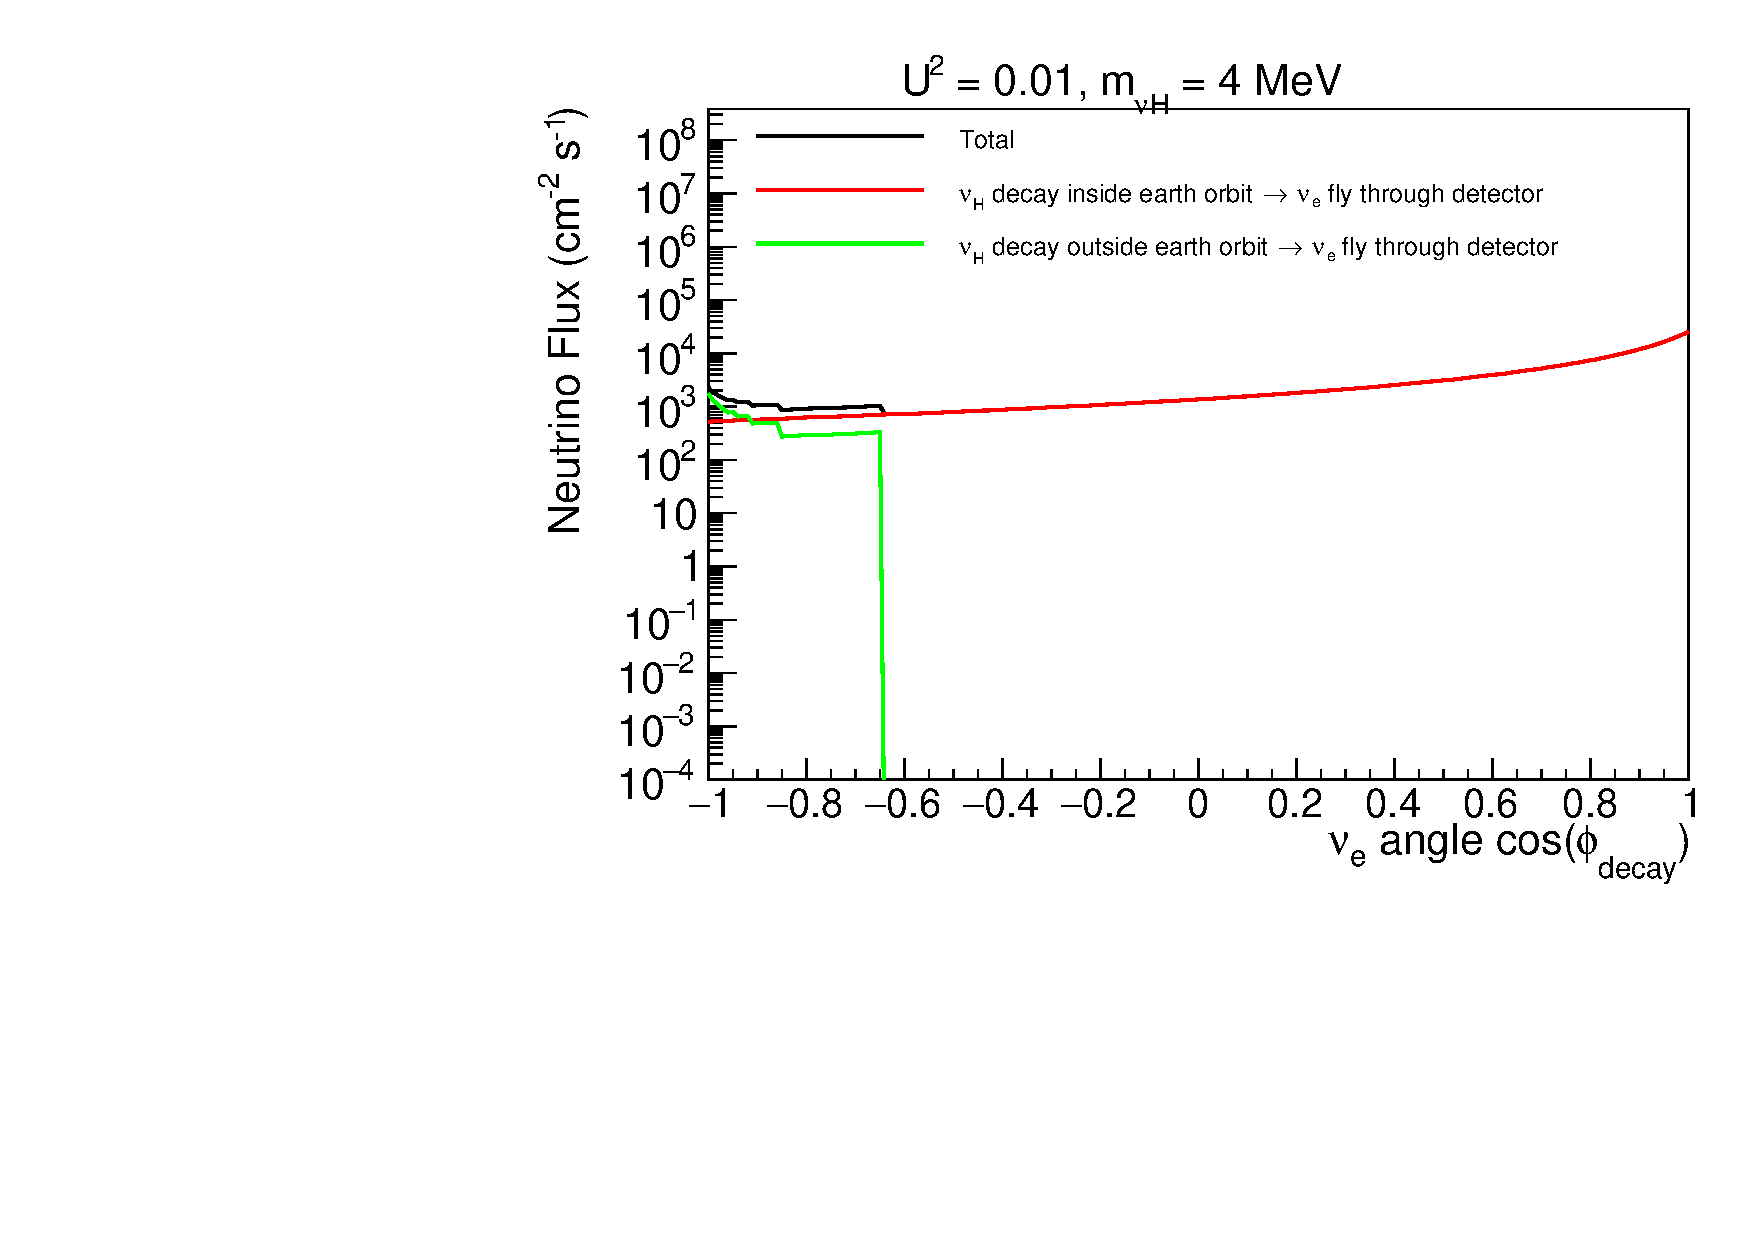
\includegraphics[width=0.99\columnwidth]{../plots/DecayInFlightNuLCosphiSun_U0.01_M4.0_InsideOutside_linXlogY.pdf}
\caption{Distributions of emission angle $\cos(\phi_{decay})$ of $\nu_e$'s that come from $\nu_H$ decay in flight and then reach the detector on earth. The distributions for $\nu_H$ decay inside and outside earth orbit are shown separately. The signal model shown in this plot is $m_{\nu H} = 4$ MeV and $|U_{eH}|^2 = 10^{-2}$.}
\label{fig:DecayInFlightPhi_U0.01_M4} 
\end{figure}


\begin{figure}[!htbp]
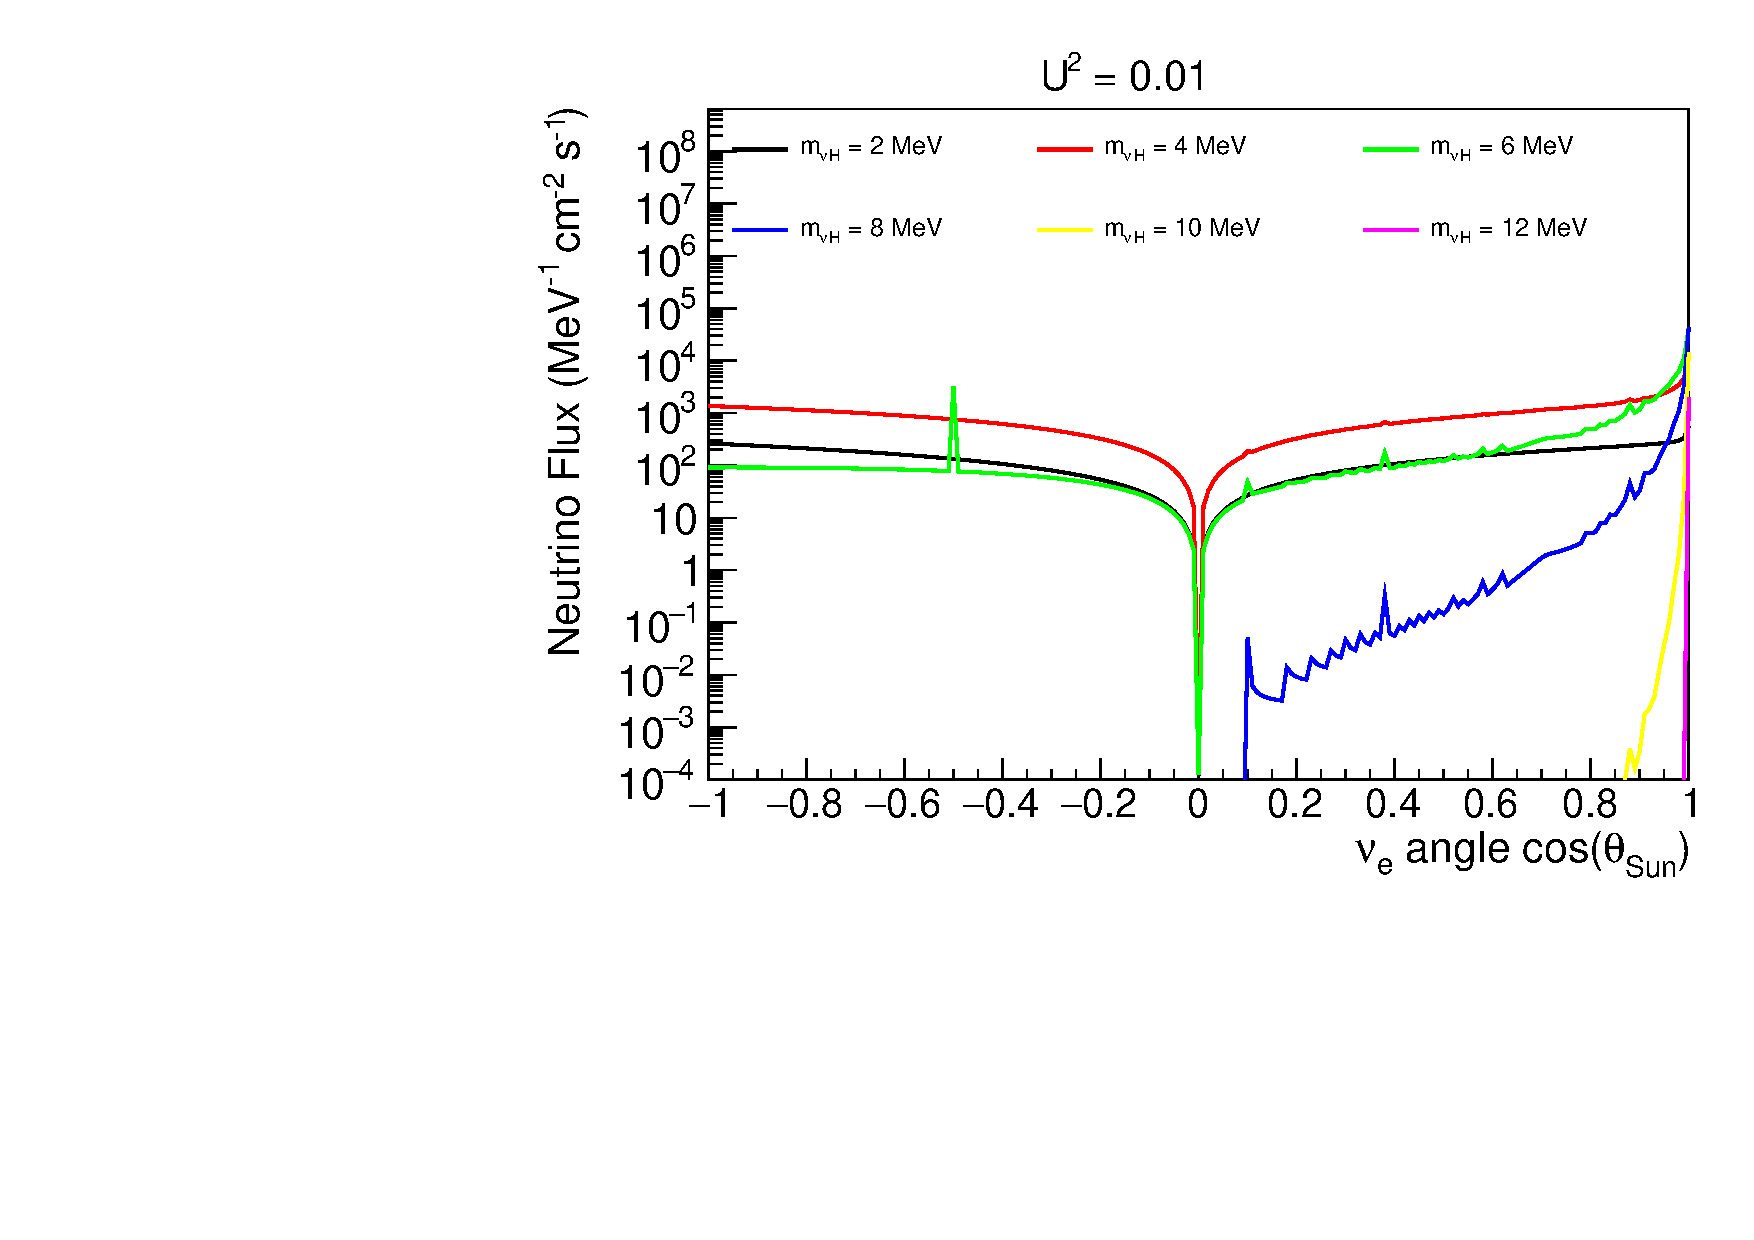
\includegraphics[width=0.99\columnwidth]{../plots/DecayInFlightNuLCosthetaSun_U0.01_AllMass_linXlogY.pdf}
\caption{Distributions of solar angle $\cos(\theta_{Sun})$ of $\nu_e$'s that come from $\nu_H$ decay in flight and then reach the detector on earth. Different curves are for different $\nu_H$ masses $m_{\nu H}$, and the mixing angle $|U_{eH}|^2 = 10^{-2}$.}
\label{fig:DecayInFlightTheta_U1em2_AllMass}
\end{figure}

\begin{figure}[!htbp]
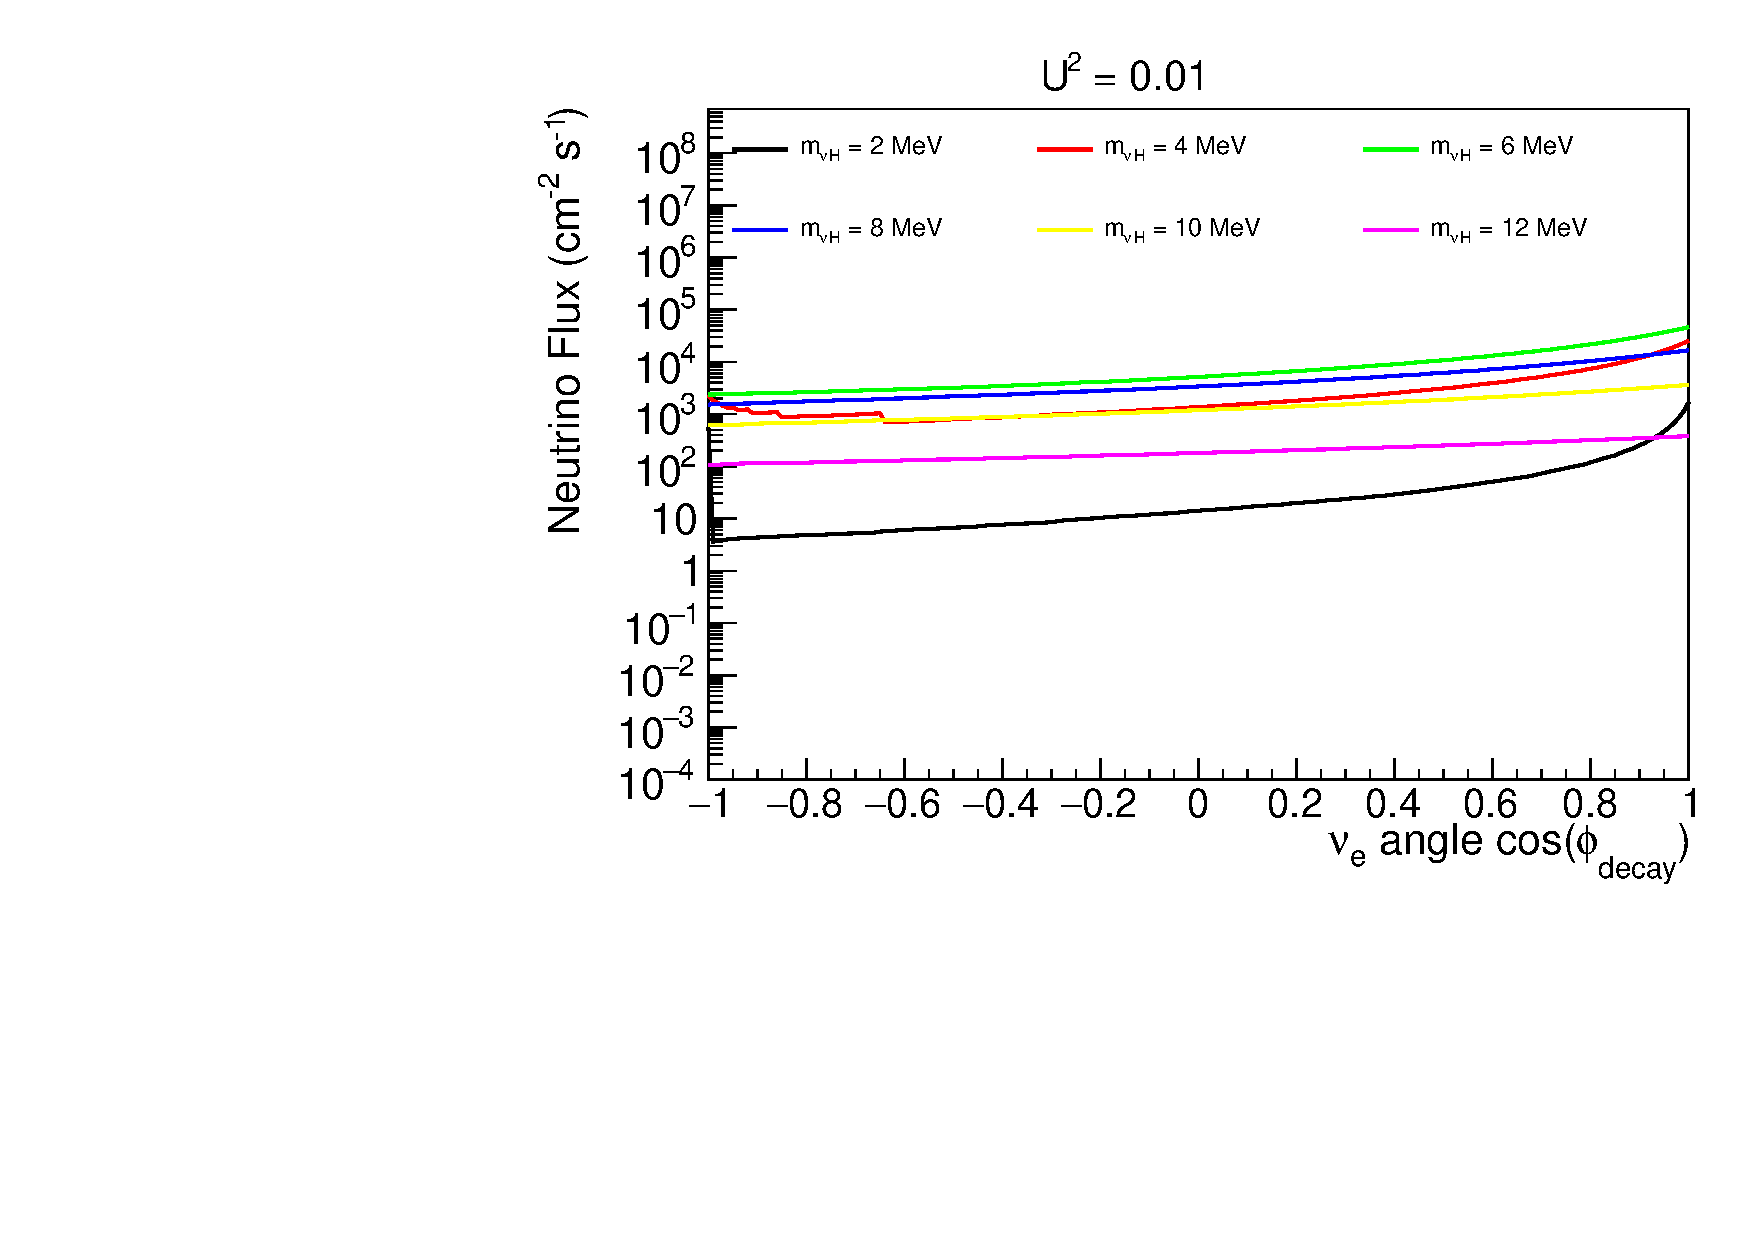
\includegraphics[width=0.99\columnwidth]{../plots/DecayInFlightNuLCosphiSun_U0.01_AllMass_linXlogY.pdf}
\caption{Distributions of emission angle $\cos(\phi_{decay})$ of $\nu_e$'s that come from $\nu_H$ decay in flight and then reach the detector on earth. Different curves are for different $\nu_H$ masses $m_{\nu H}$, and the mixing angle $|U_{eH}|^2 = 10^{-2}$.}
\label{fig:DecayInFlightPhi_U1em2_AllMass}
\end{figure}

\begin{figure}[!htbp]
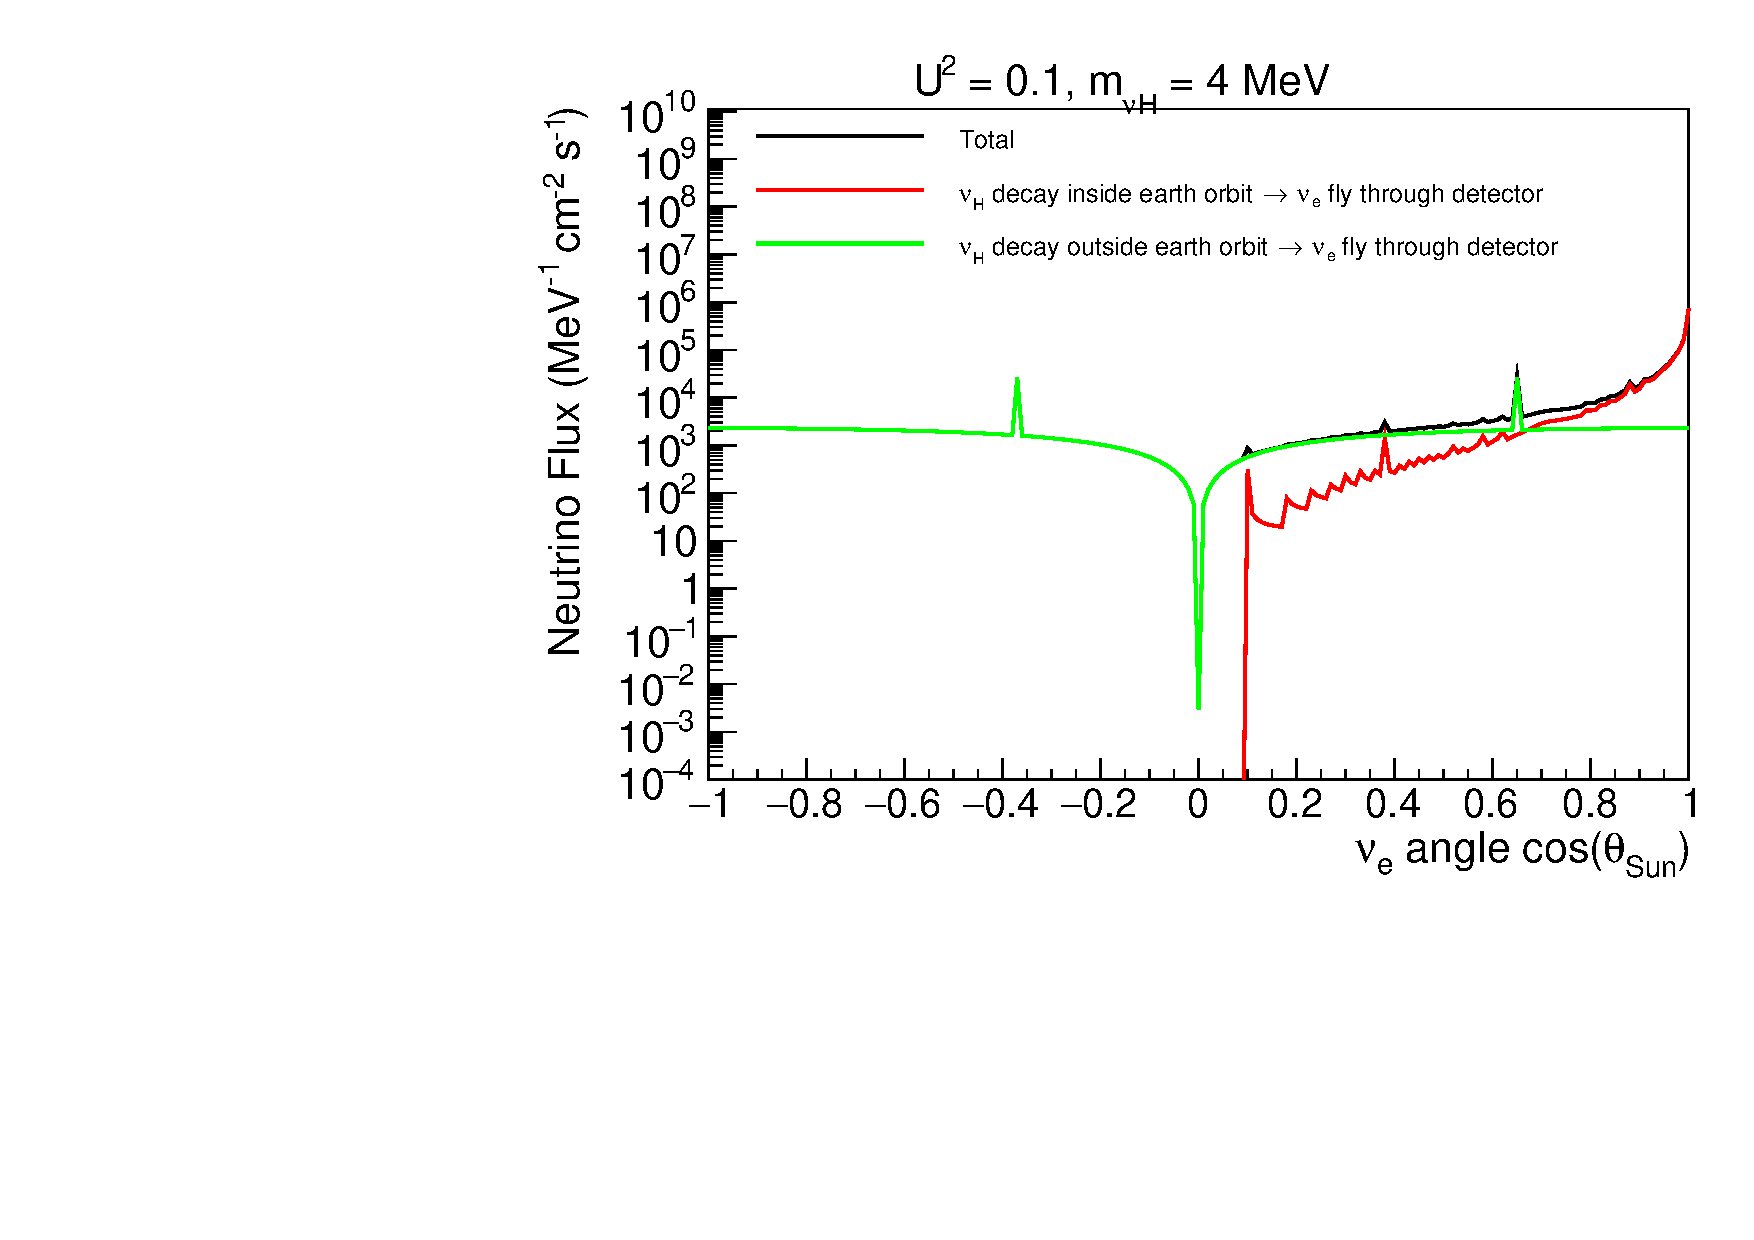
\includegraphics[width=0.99\columnwidth]{../plots/DecayInFlightNuLCosthetaSun_U0.1_M4.0_InsideOutside_linXlogY.pdf}
\caption{Distribution solar angle $\cos(\theta_{Sun})$ of $\nu_e$'s that come from $\nu_H$ decay in flight and then reach the detector on earth. The distributions for $\nu_H$ decay inside and outside earth orbit are shown separately. The signal model shown in this plot is $m_{\nu H} = 4$ MeV and $|U_{eH}|^2 = 10^{-1}$.}
\label{fig:DecayInFlightTheta_U0.1_M4} 
\end{figure}


\begin{figure}[!htbp]
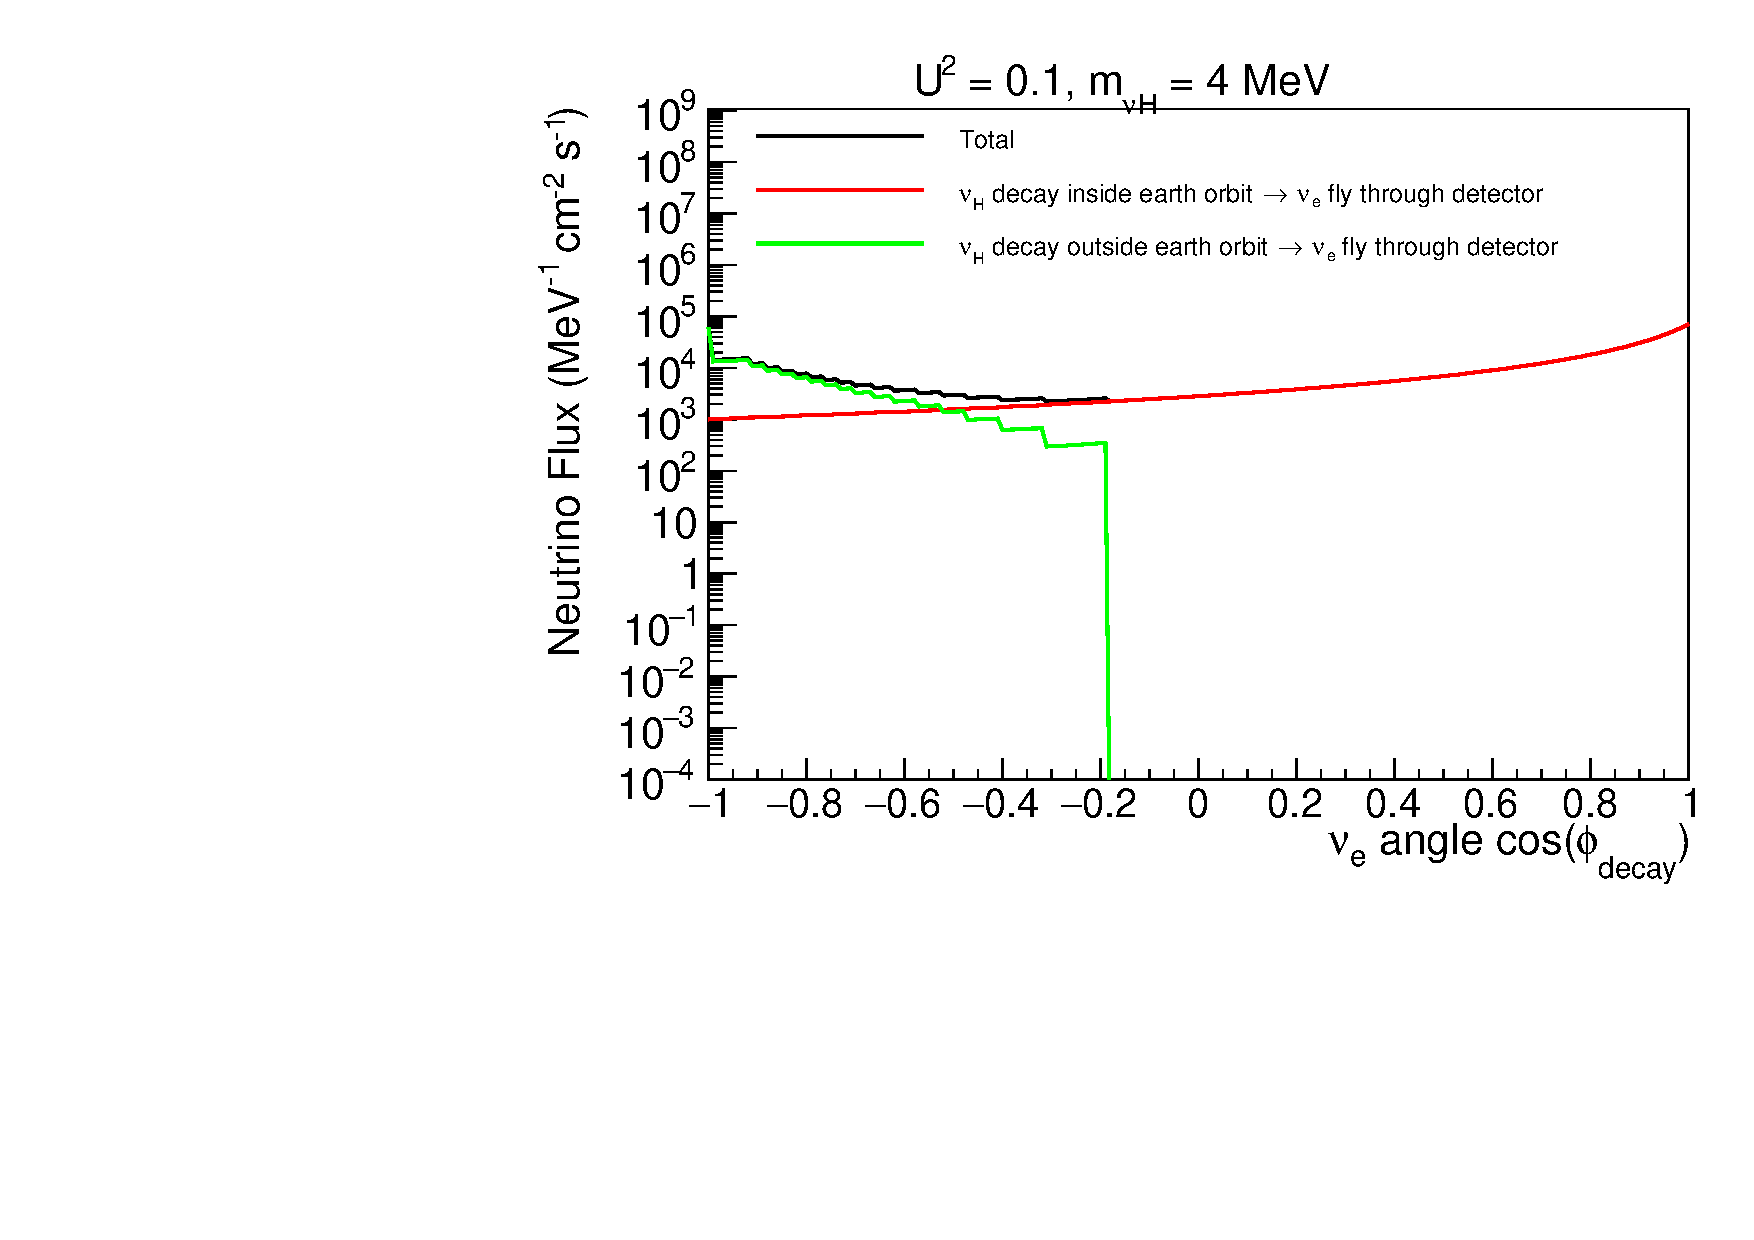
\includegraphics[width=0.99\columnwidth]{../plots/DecayInFlightNuLCosphiSun_U0.1_M4.0_InsideOutside_linXlogY.pdf}
\caption{Distributions of emission angle $\cos(\phi_{decay})$ of $\nu_e$'s that come from $\nu_H$ decay in flight and then reach the detector on earth. The distributions for $\nu_H$ decay inside and outside earth orbit are shown separately. The signal model shown in this plot is $m_{\nu H} = 4$ MeV and $|U_{eH}|^2 = 10^{-1}$.}
\label{fig:DecayInFlightPhi_U0.1_M4} 
\end{figure}


\begin{figure}[!htbp]
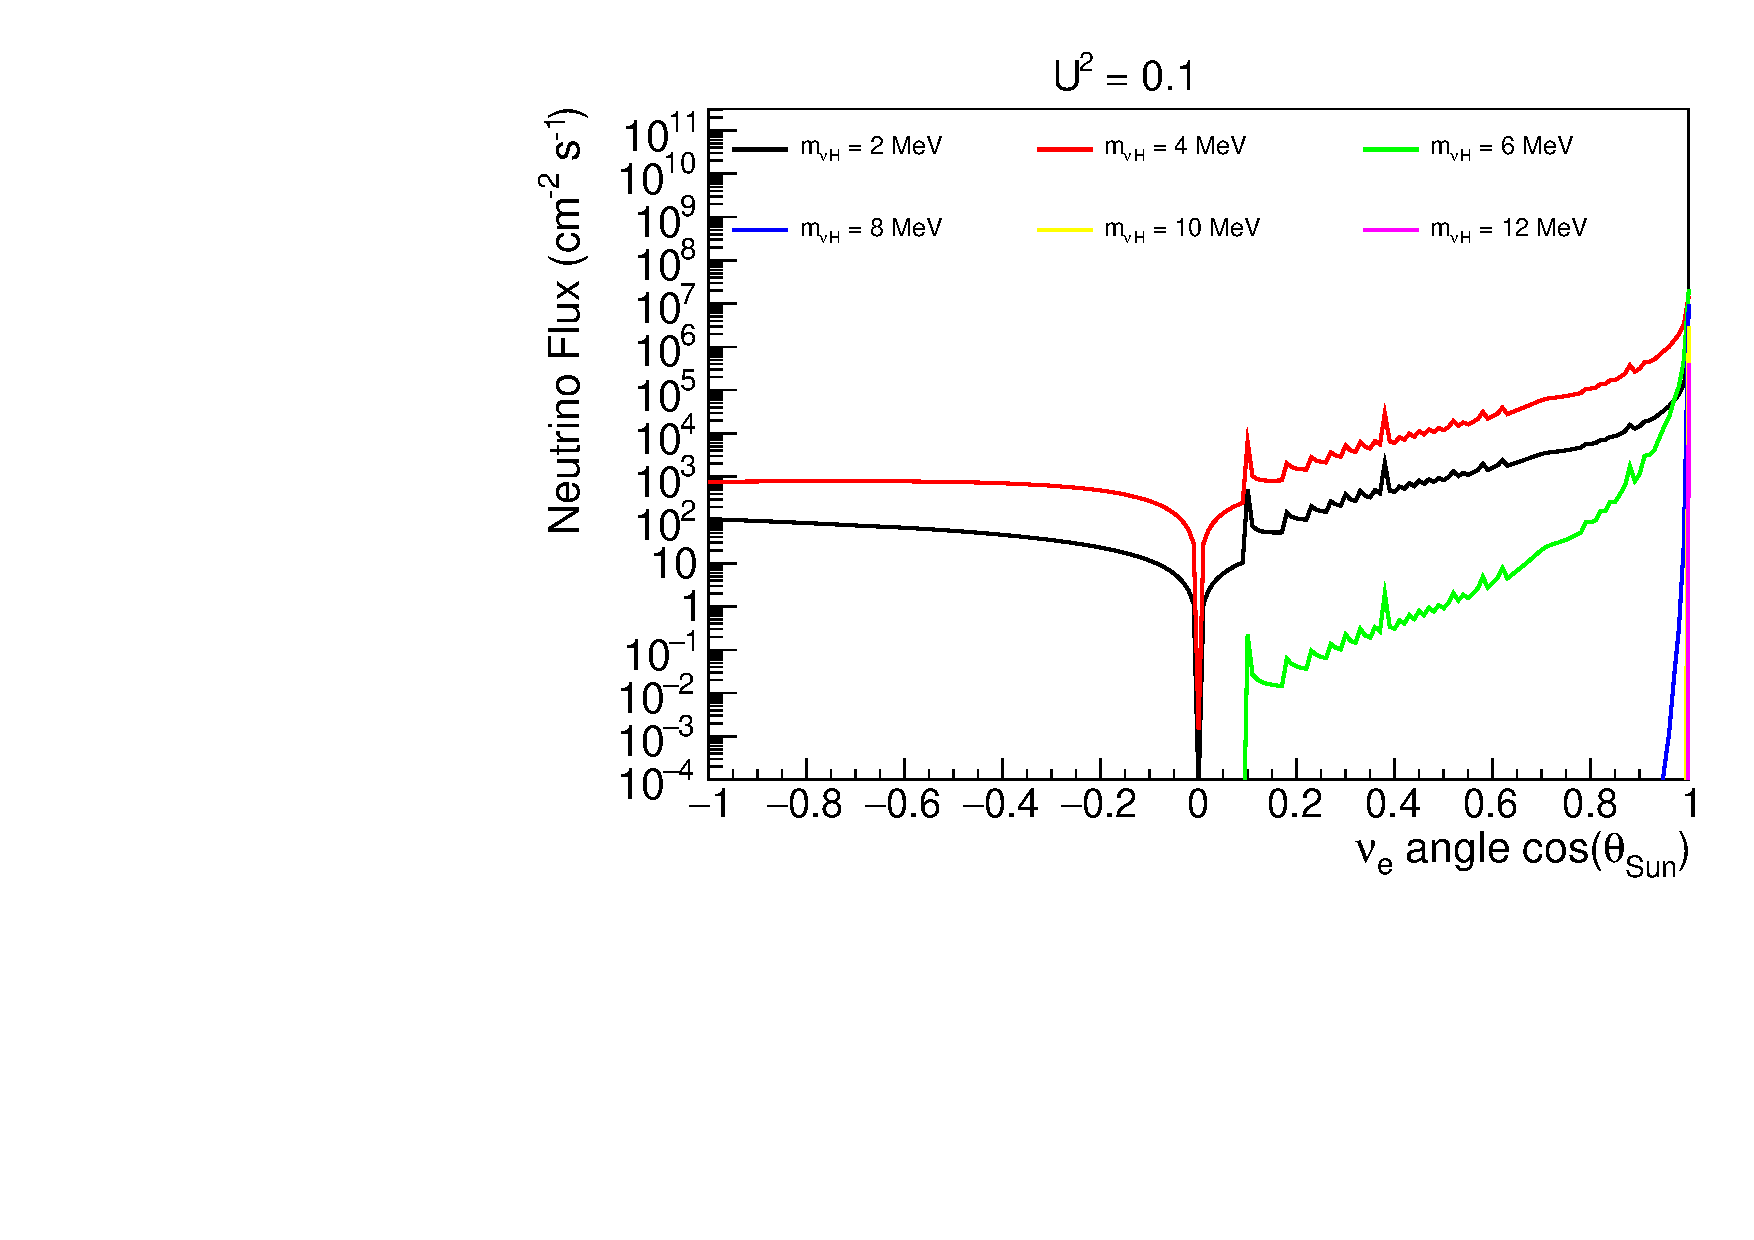
\includegraphics[width=0.99\columnwidth]{../plots/DecayInFlightNuLCosthetaSun_U0.1_AllMass_linXlogY.pdf}
\caption{Distributions of solar angle $\cos(\theta_{Sun})$ of $\nu_e$'s that come from $\nu_H$ decay in flight and then reach the detector on earth. Different curves are for different $\nu_H$ masses $m_{\nu H}$, and the mixing angle $|U_{eH}|^2 = 10^{-1}$.}
\label{fig:DecayInFlightTheta_U1em1_AllMass}
\end{figure}

\begin{figure}[!htbp]
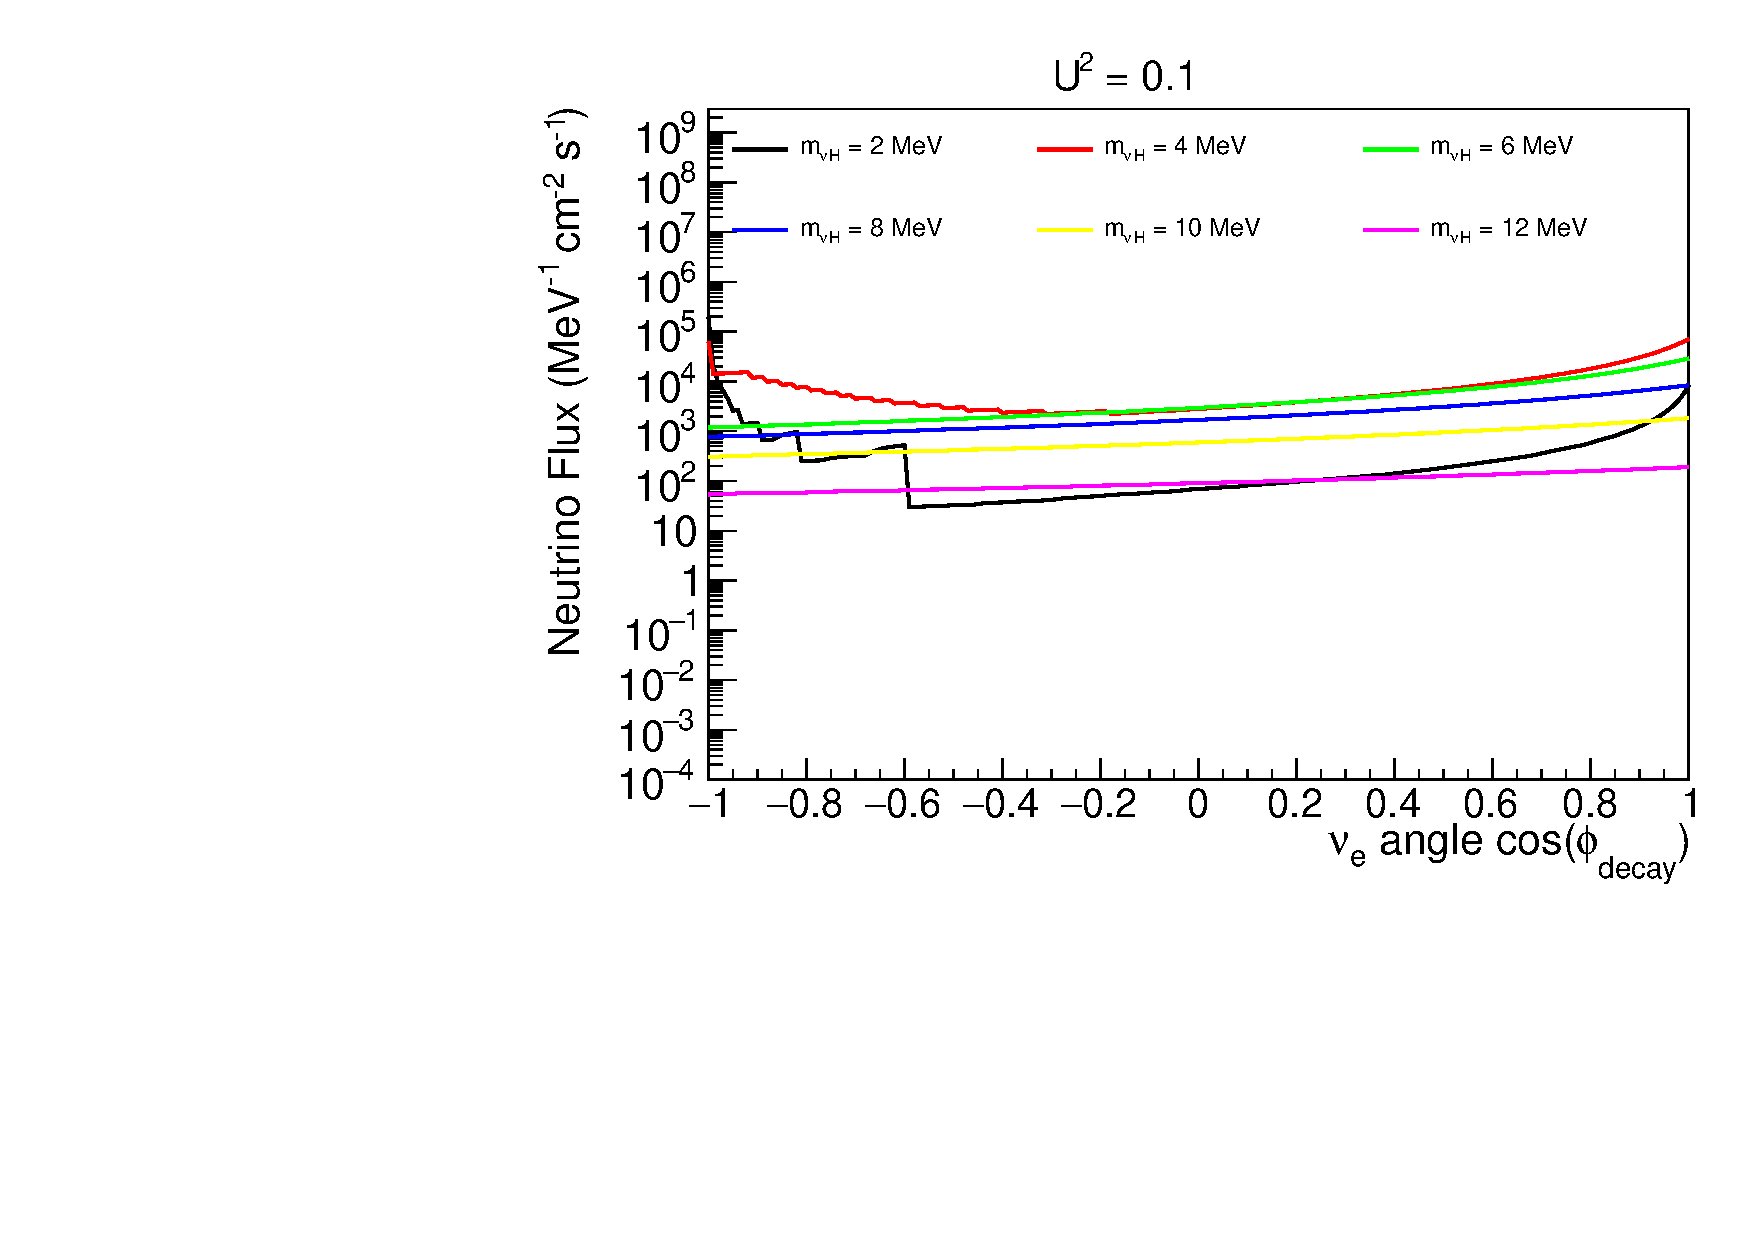
\includegraphics[width=0.99\columnwidth]{../plots/DecayInFlightNuLCosphiSun_U0.1_AllMass_linXlogY.pdf}
\caption{Distributions of emission angle $\cos(\phi_{decay})$ of $\nu_e$'s that come from $\nu_H$ decay in flight and then reach the detector on earth. Different curves are for different $\nu_H$ masses $m_{\nu H}$, and the mixing angle $|U_{eH}|^2 = 10^{-1}$.}
\label{fig:DecayInFlightPhi_U1em1_AllMass}
\end{figure}

\begin{figure}[!htbp]
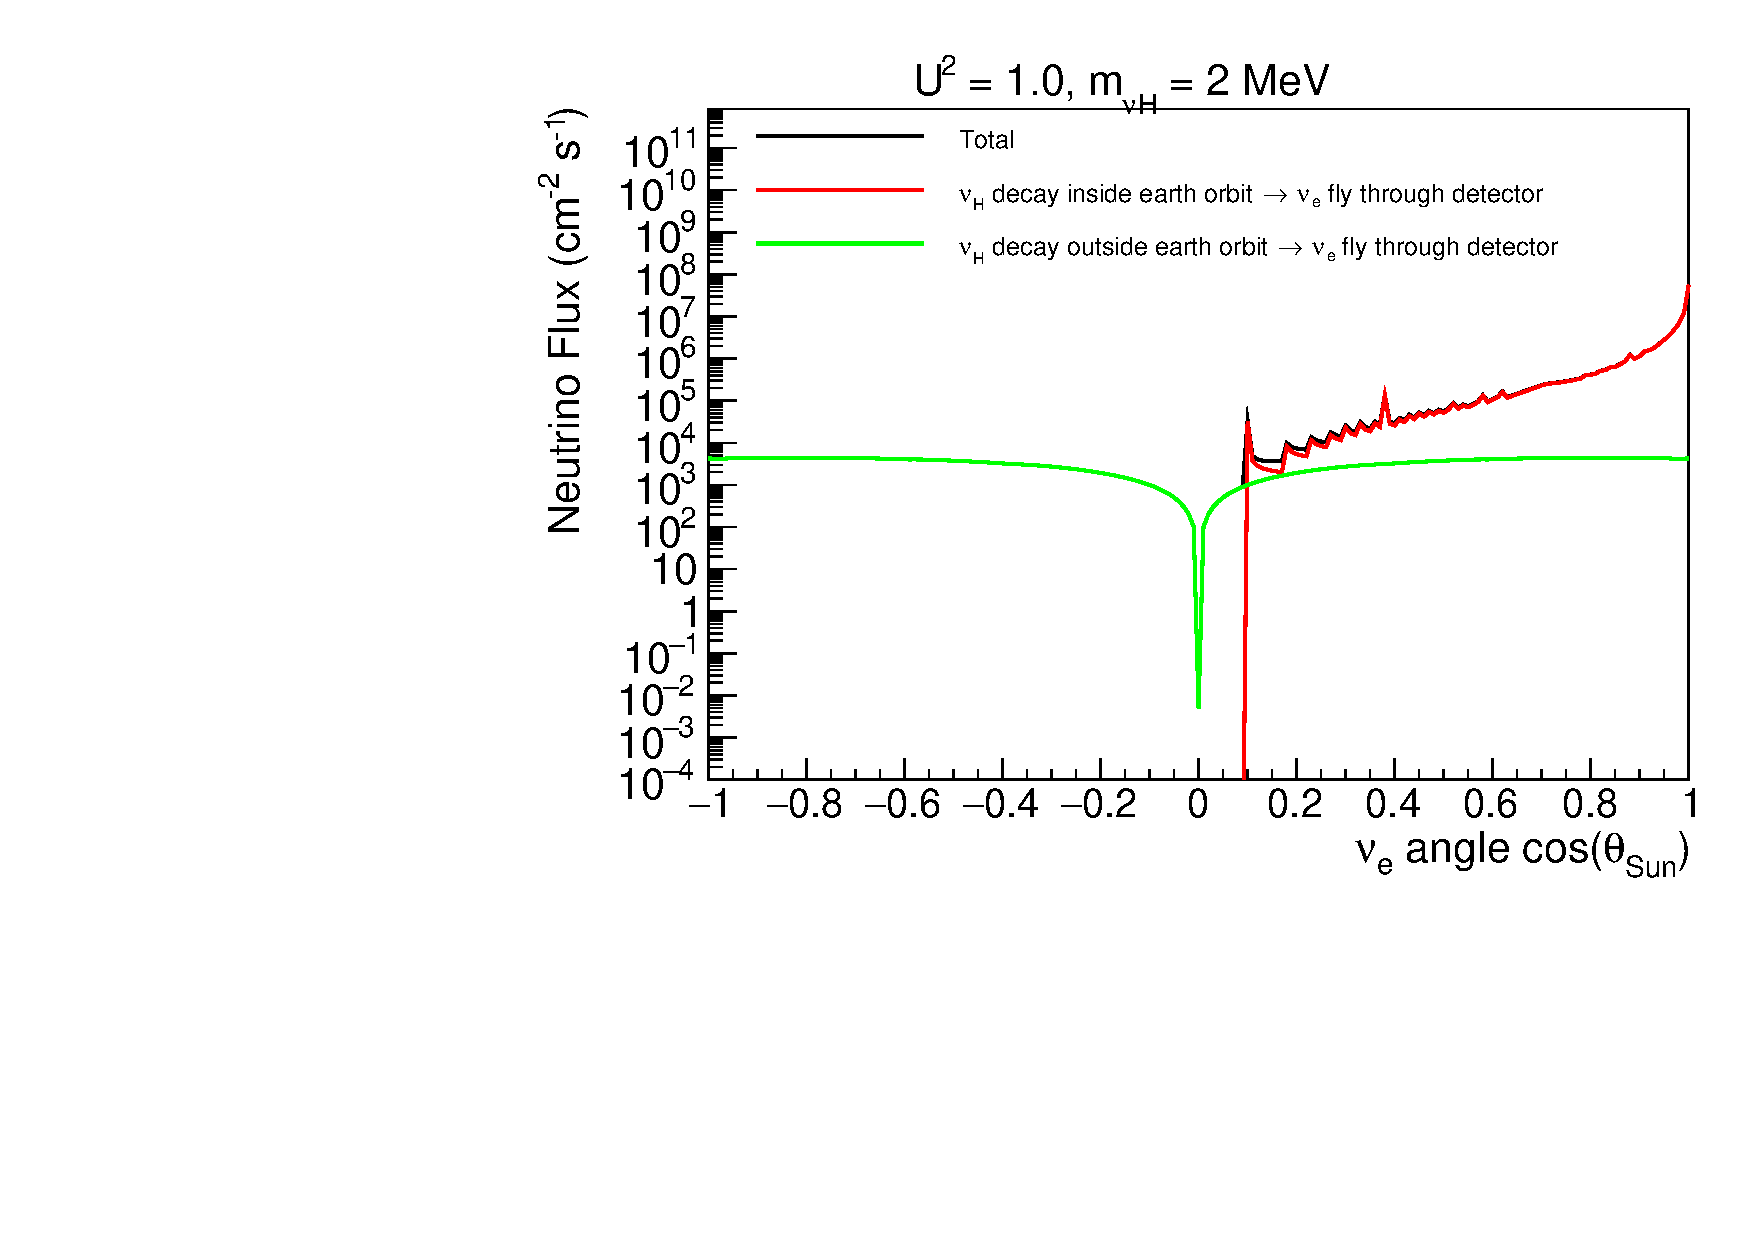
\includegraphics[width=0.99\columnwidth]{../plots/DecayInFlightNuLCosthetaSun_U1.0_M2.0_InsideOutside_linXlogY.pdf}
\caption{Distribution solar angle $\cos(\theta_{Sun})$ of $\nu_e$'s that come from $\nu_H$ decay in flight and then reach the detector on earth. The distributions for $\nu_H$ decay inside and outside earth orbit are shown separately. The signal model shown in this plot is $m_{\nu H} = 2$ MeV and $|U_{eH}|^2 = 1.0$.}
\label{fig:DecayInFlightTheta_U1.0_M2} 
\end{figure}


\begin{figure}[!htbp]
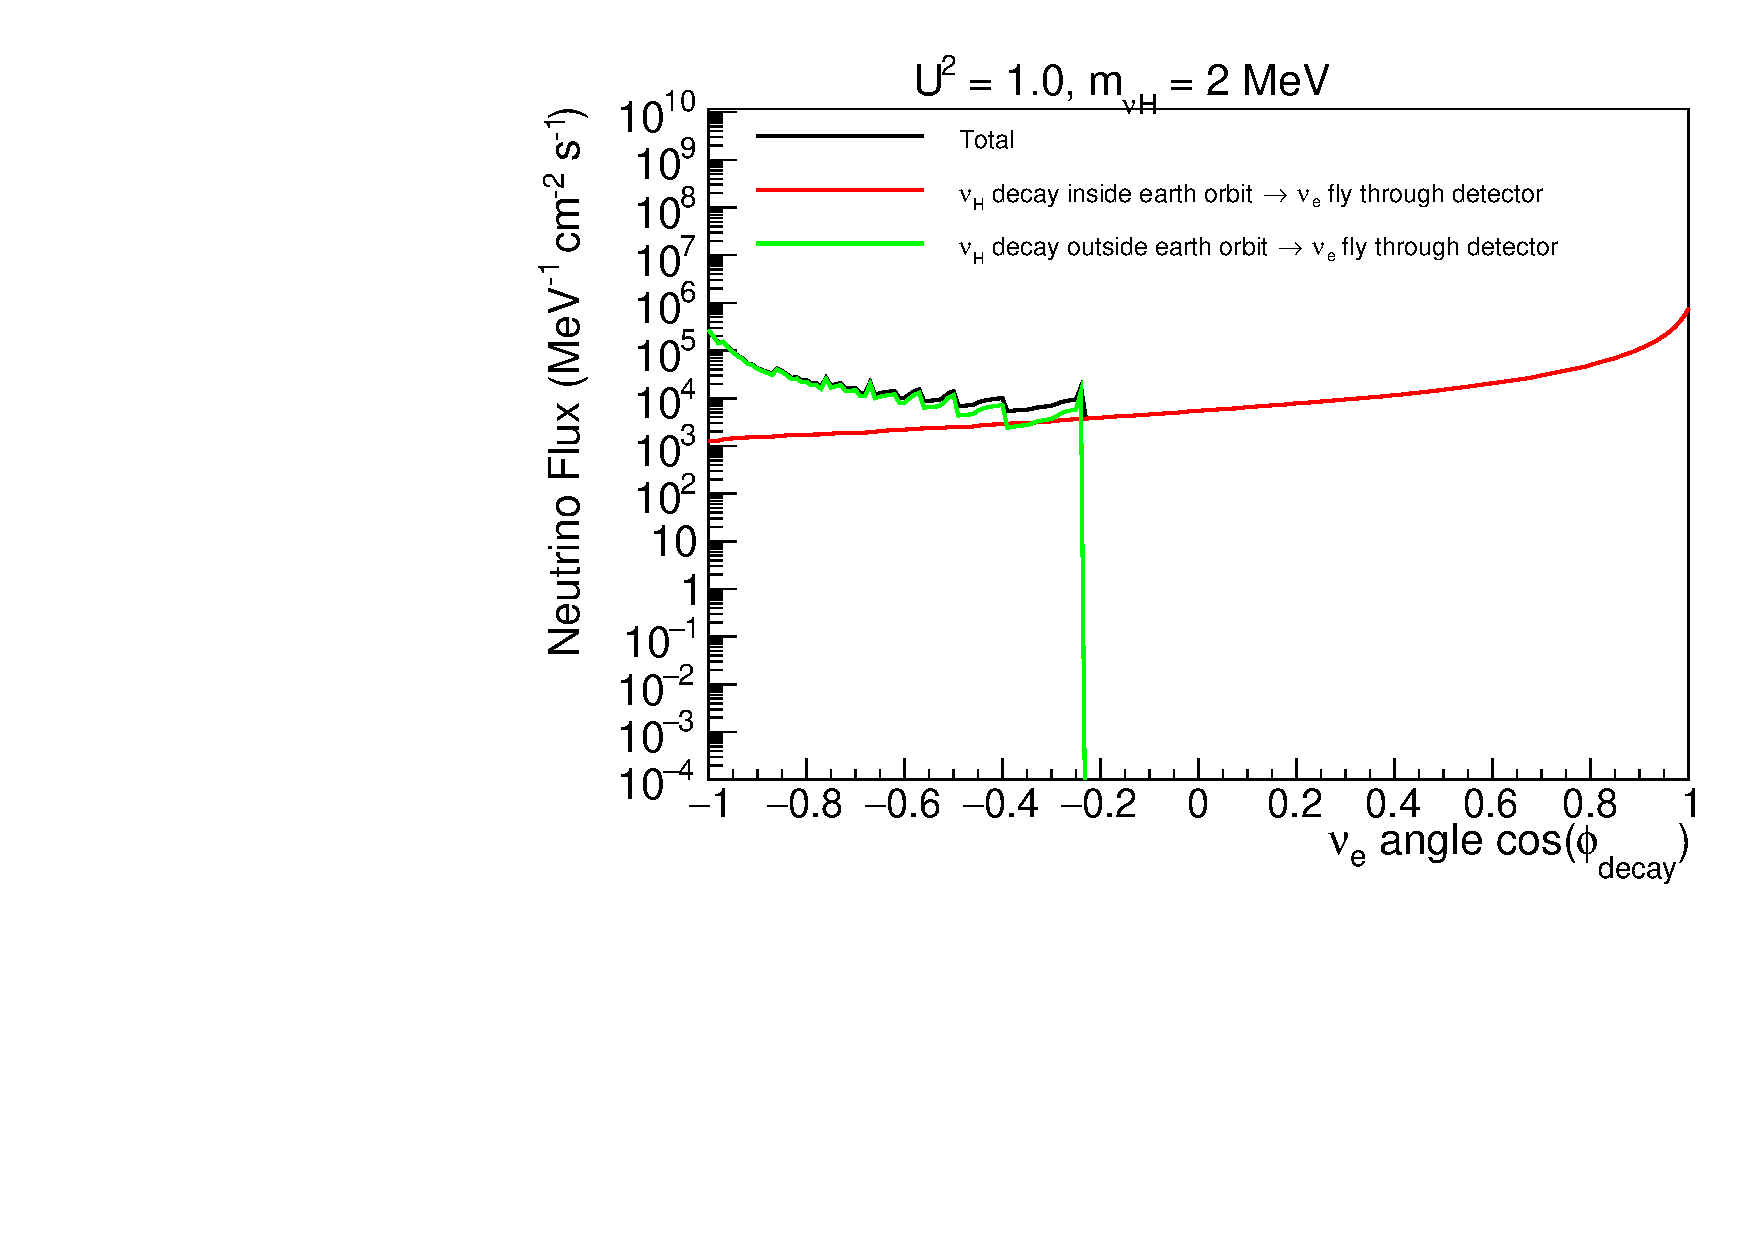
\includegraphics[width=0.99\columnwidth]{../plots/DecayInFlightNuLCosphiSun_U1.0_M2.0_InsideOutside_linXlogY.pdf}
\caption{Distributions of emission angle $\cos(\phi_{decay})$ of $\nu_e$'s that come from $\nu_H$ decay in flight and then reach the detector on earth. The distributions for $\nu_H$ decay inside and outside earth orbit are shown separately. The signal model shown in this plot is $m_{\nu H} = 2$ MeV and $|U_{eH}|^2 = 1.0$.}
\label{fig:DecayInFlightPhi_U1.0_M2} 
\end{figure}



\begin{figure}[!htbp]
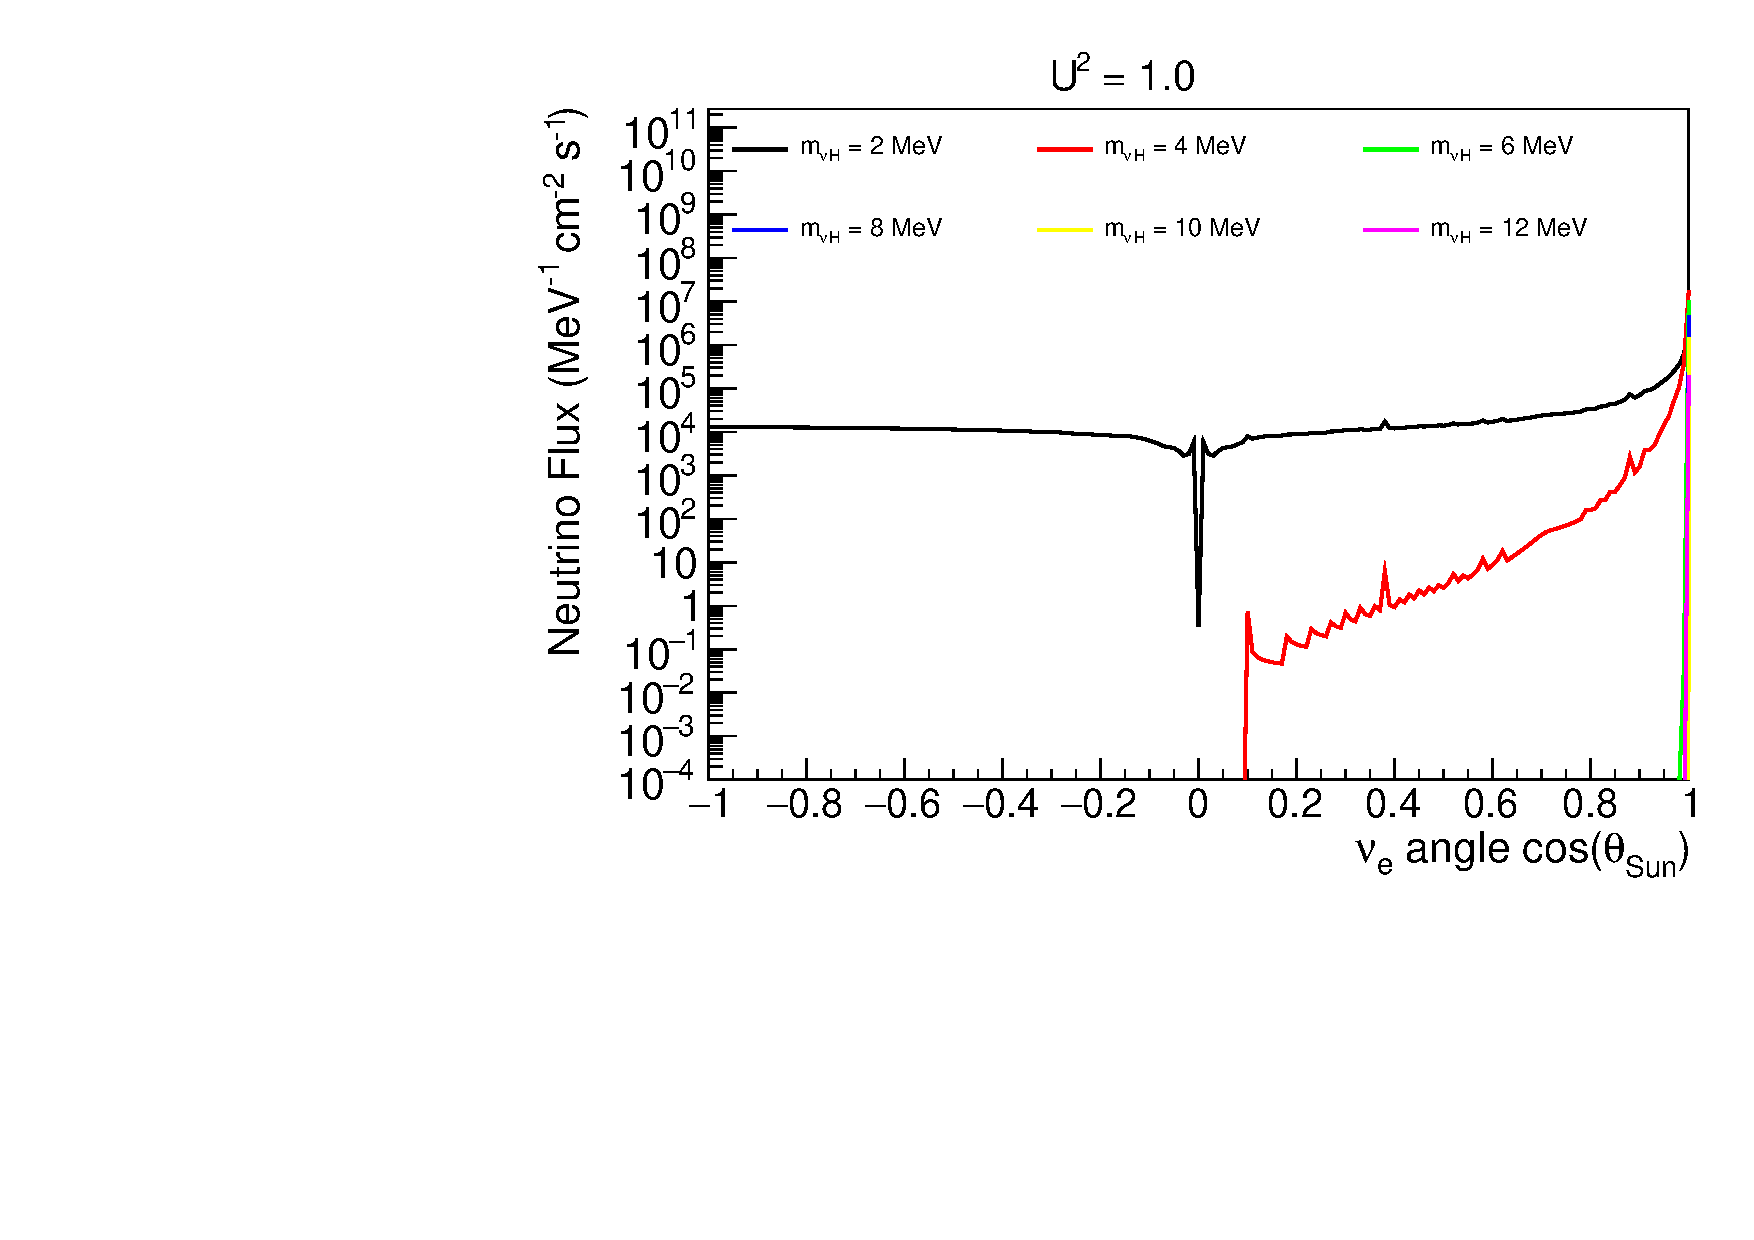
\includegraphics[width=0.99\columnwidth]{../plots/DecayInFlightNuLCosthetaSun_U1.0_AllMass_linXlogY.pdf}
\caption{Distributions of solar angle $\cos(\theta_{Sun})$ of $\nu_e$'s that come from $\nu_H$ decay in flight and then reach the detector on earth. Different curves are for different $\nu_H$ masses $m_{\nu H}$, and the mixing angle $|U_{eH}|^2 = 1$.}
\label{fig:DecayInFlightTheta_U1em0_AllMass}
\end{figure}

\begin{figure}[!htbp]
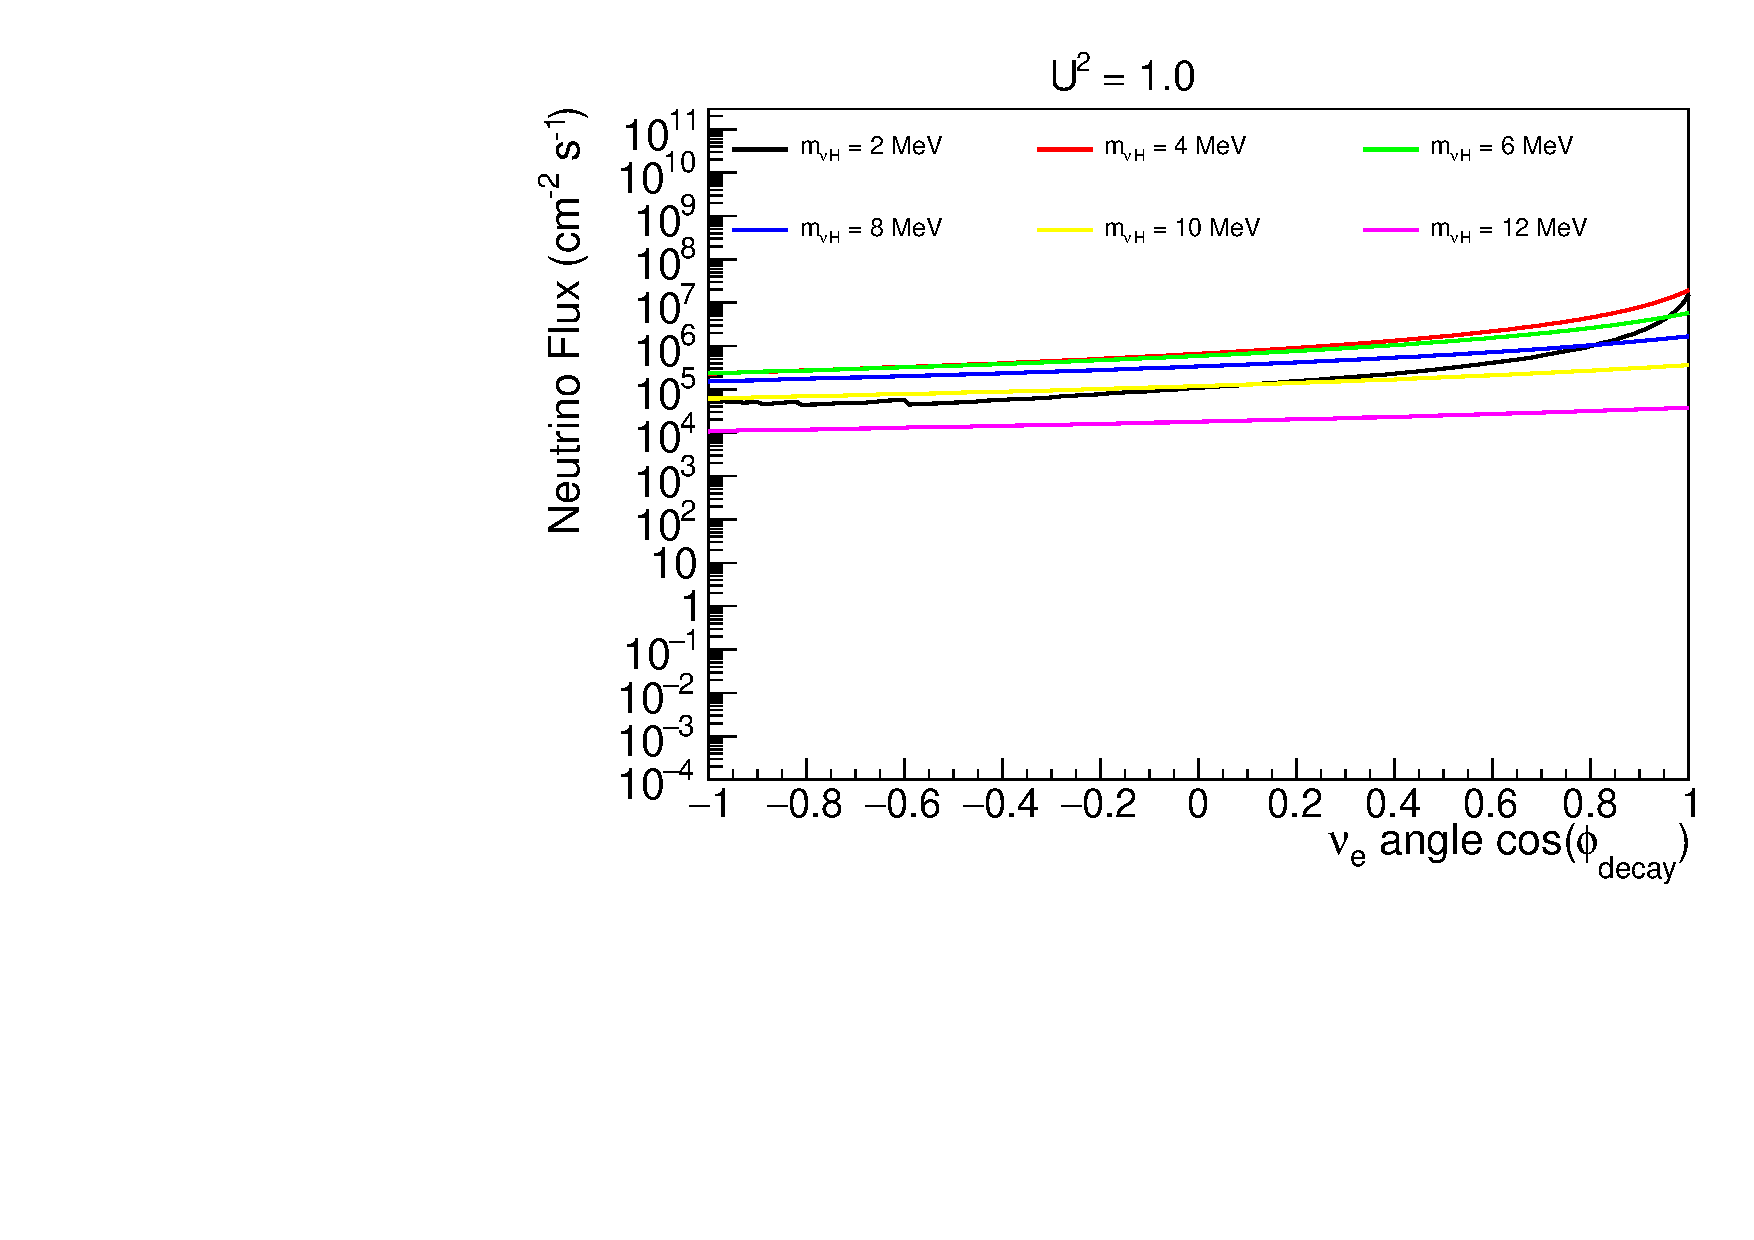
\includegraphics[width=0.99\columnwidth]{../plots/DecayInFlightNuLCosphiSun_U1.0_AllMass_linXlogY.pdf}
\caption{Distributions of emission angle $\cos(\phi_{decay})$ of $\nu_e$'s that come from $\nu_H$ decay in flight and then reach the detector on earth. Different curves are for different $\nu_H$ masses $m_{\nu H}$, and the mixing angle $|U_{eH}|^2 = 1$.}
\label{fig:DecayInFlightPhi_U1em0_AllMass}
\end{figure}

\clearpage

\section{\label{sec:NueSpectrum} Search for $\nu_H$ with $\nu_e$ spectrum}

\begin{figure}[!htbp]
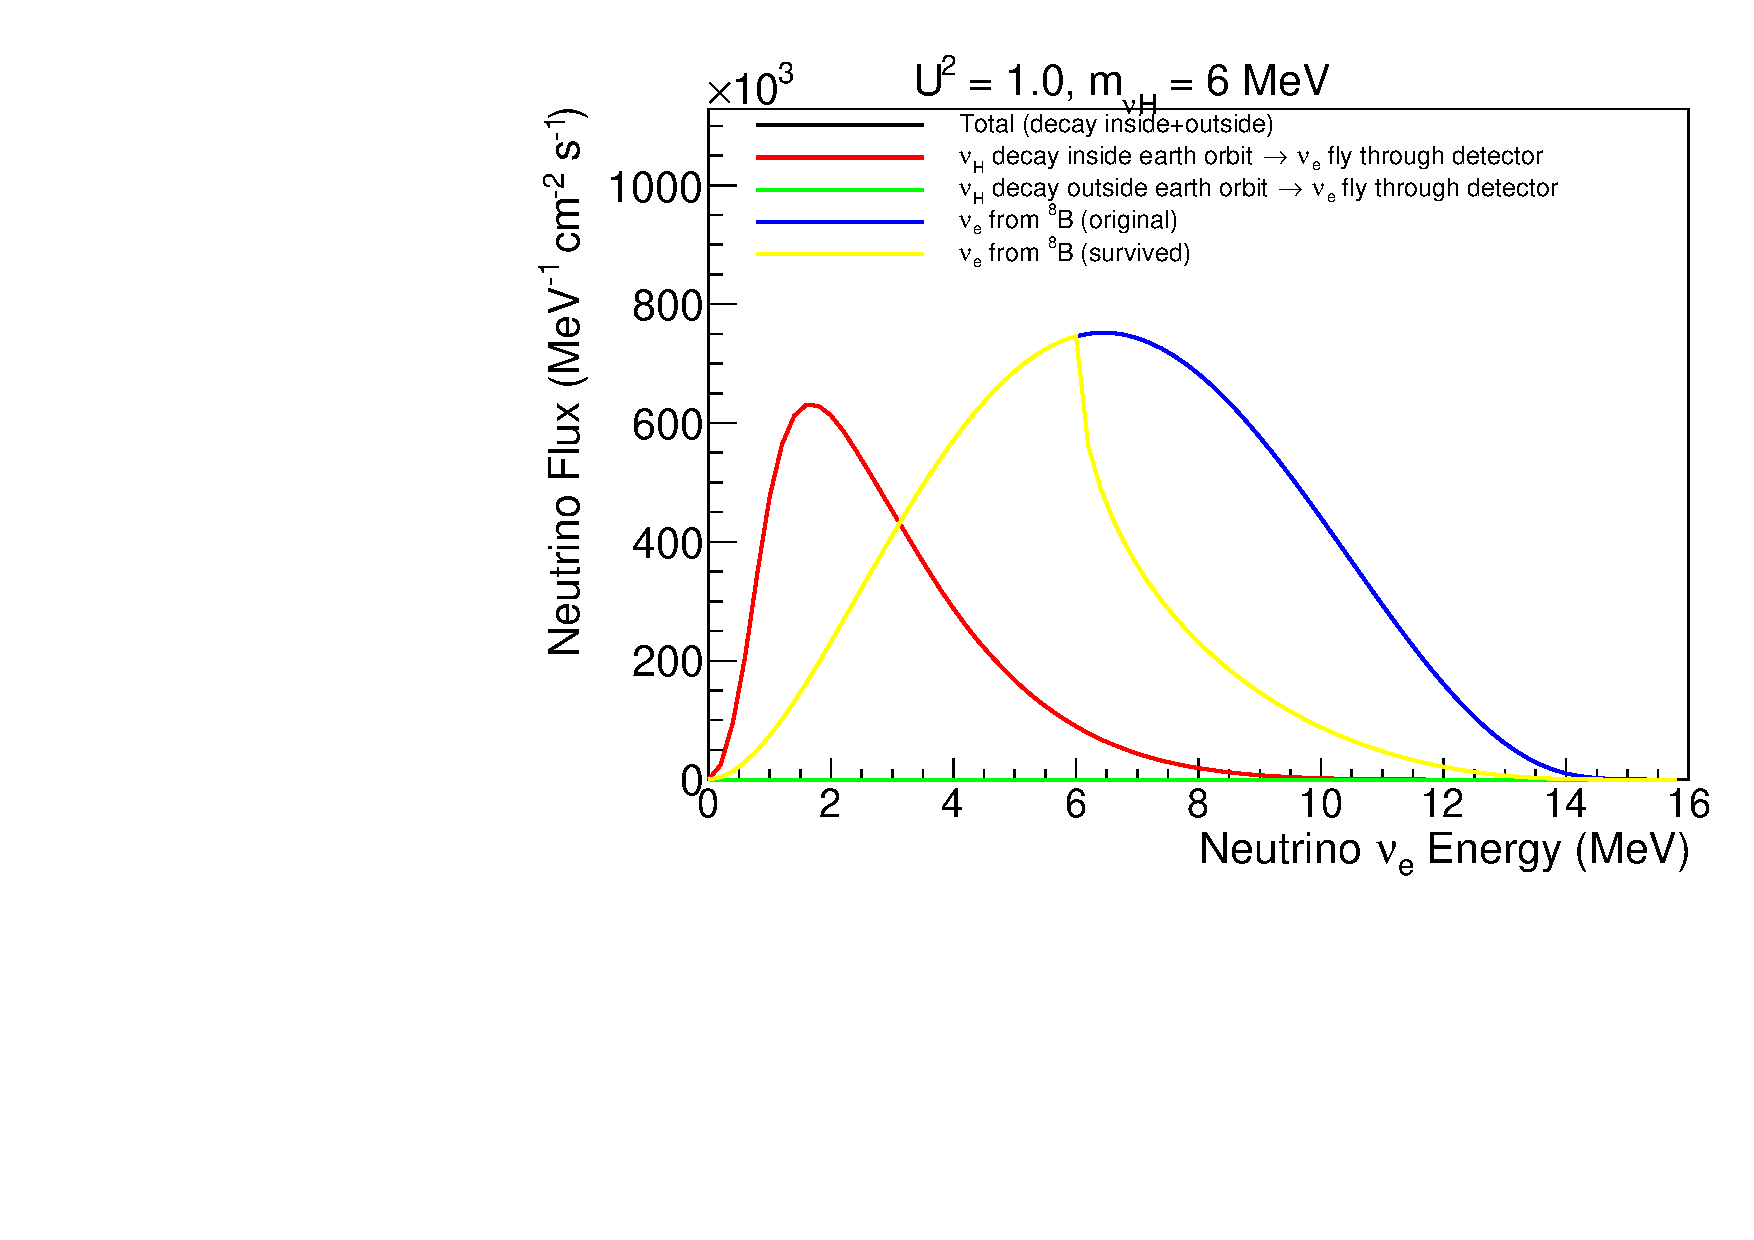
\includegraphics[width=0.99\columnwidth]{../plots/DecayInFlightNuLEnergy_U1.0_M6.0_InsideOutside_linXlinY.pdf}
\caption{Energy spectra of $\nu_e$'s that come from $\nu_H$ decay in flight and then reach the detector on earth. The spectra for $\nu_H$ decay inside and outside earth orbit are shown separately. 
The original solar neutrino spectrum that come from $^8 B$ decay in the Sun, and spectrum of solar neutrino that survived the mix to $\nu_H$ during $^{8}B$ decay, are also shown in the plot. The signal model shown in this plot is $m_{\nu H} = 6$ MeV and $|U_{eH}|^2 = 1.0$.}
\label{fig:DecayInFlightSpectrum_U_M6} 
\end{figure}

\begin{figure}[!htbp]
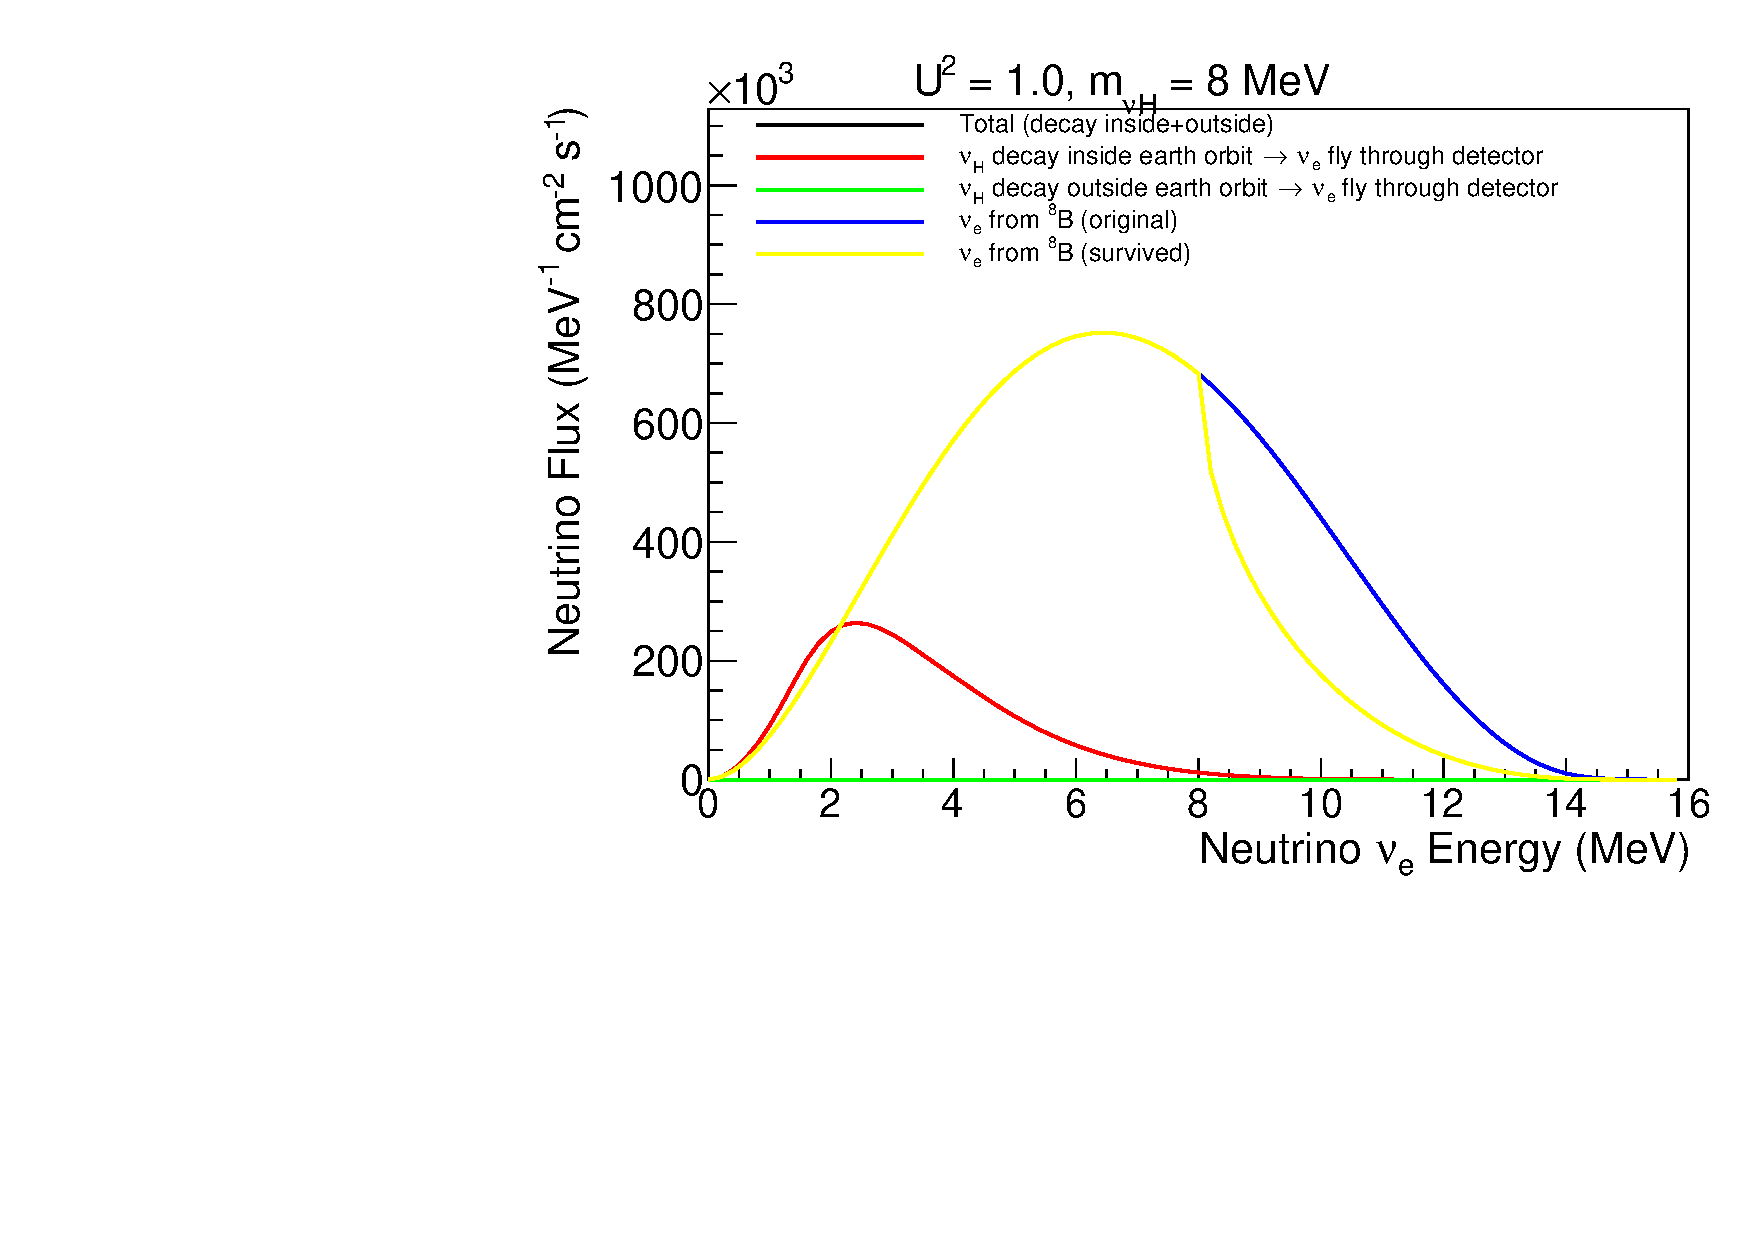
\includegraphics[width=0.99\columnwidth]{../plots/DecayInFlightNuLEnergy_U1.0_M8.0_InsideOutside_linXlinY.pdf}
\caption{Energy spectra of $\nu_e$'s that come from $\nu_H$ decay in flight and then reach the detector on earth. The spectra for $\nu_H$ decay inside and outside earth orbit are shown separately. 
The original solar neutrino spectrum that come from $^8 B$ decay in the Sun, and spectrum of solar neutrino that survived the mix to $\nu_H$ during $^{8}B$ decay, are also shown in the plot. The signal model shown in this plot is $m_{\nu H} = 8$ MeV and $|U_{eH}|^2 = 1.0$.}
\label{fig:DecayInFlightSpectrum_U_M8} 
\end{figure}


\begin{figure}[!htbp]
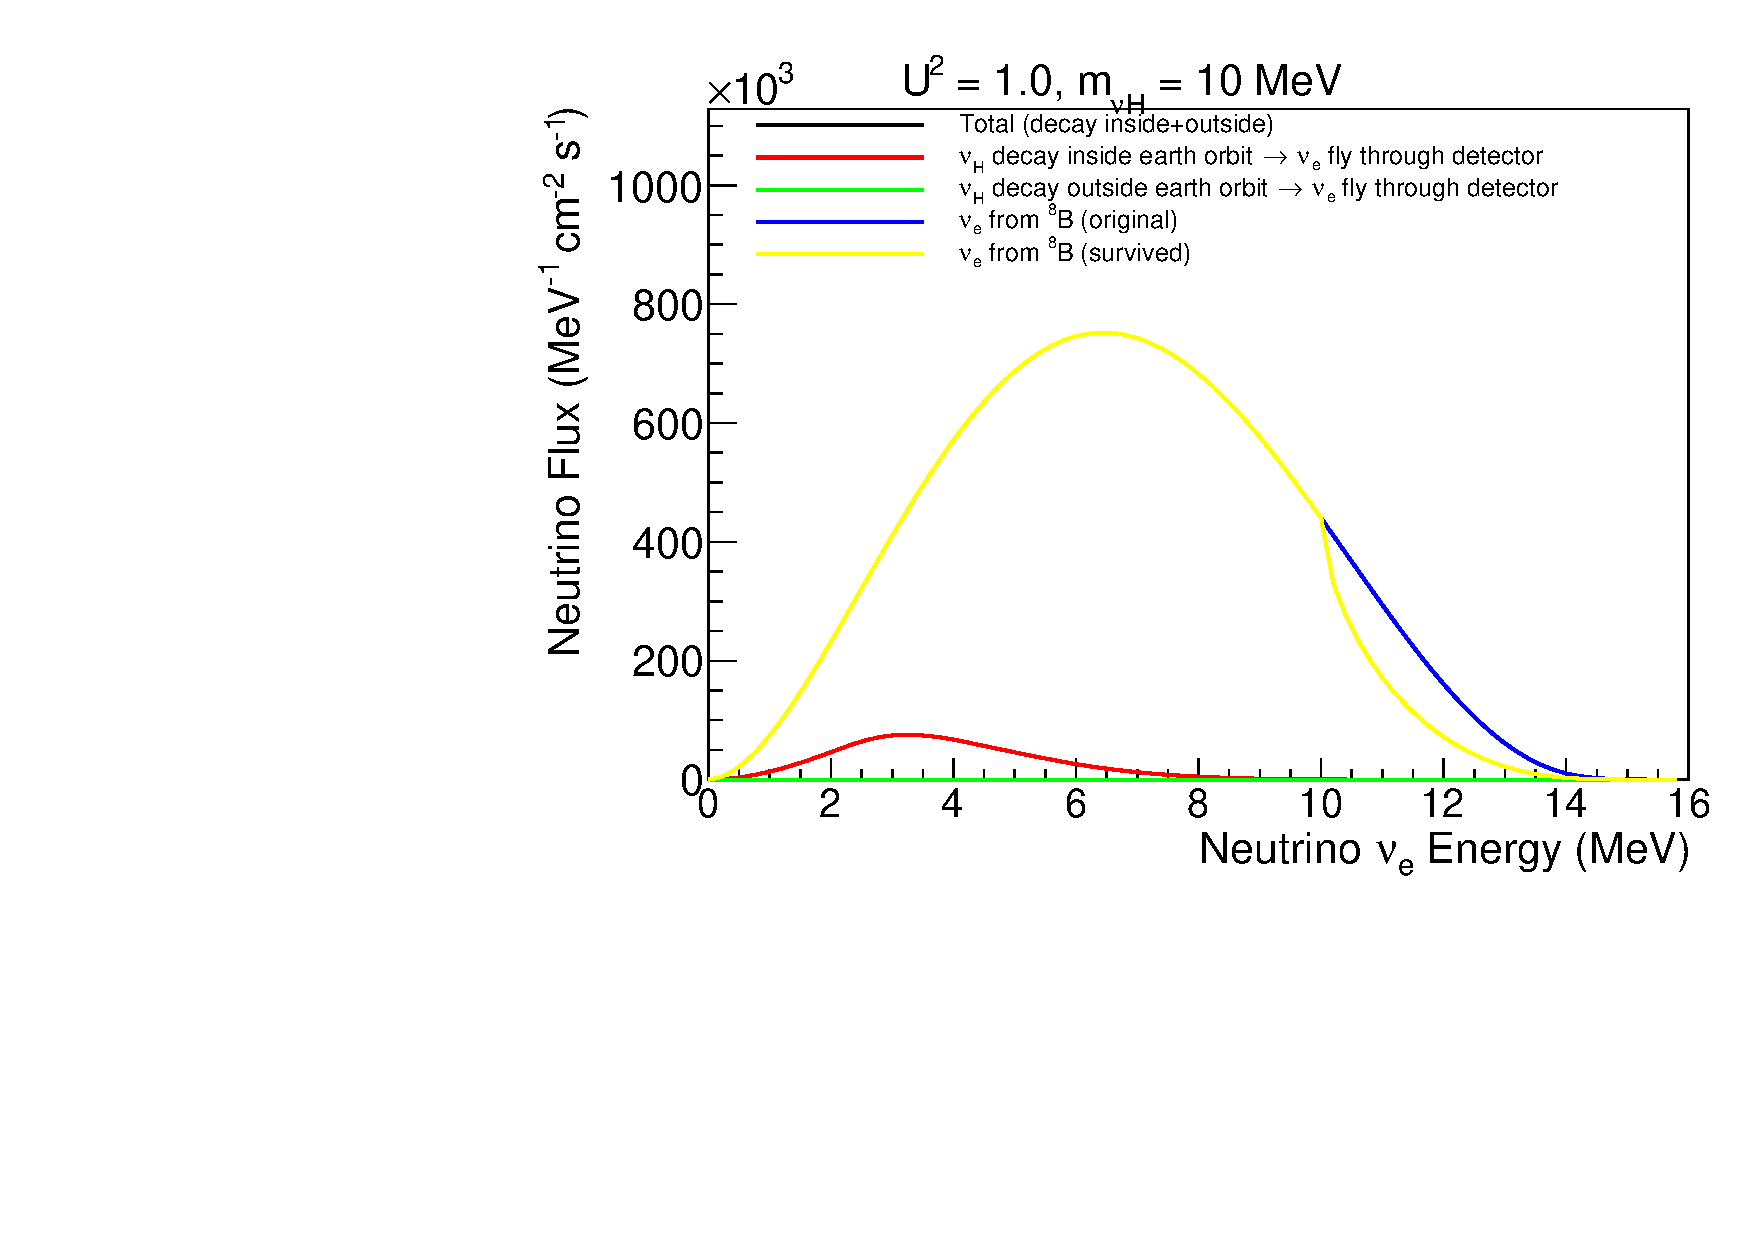
\includegraphics[width=0.99\columnwidth]{../plots/DecayInFlightNuLEnergy_U1.0_M10.0_InsideOutside_linXlinY.pdf}
\caption{Energy spectra of $\nu_e$'s that come from $\nu_H$ decay in flight and then reach the detector on earth. The spectra for $\nu_H$ decay inside and outside earth orbit are shown separately. 
The original solar neutrino spectrum that come from $^8 B$ decay in the Sun, and spectrum of solar neutrino that survived the mix to $\nu_H$ during $^{8}B$ decay, are also shown in the plot. The signal model shown in this plot is $m_{\nu H} = 10$ MeV and $|U_{eH}|^2 = 1.0$.}
\label{fig:DecayInFlightSpectrum_U1_M10} 
\end{figure}


\begin{figure}[!htbp]
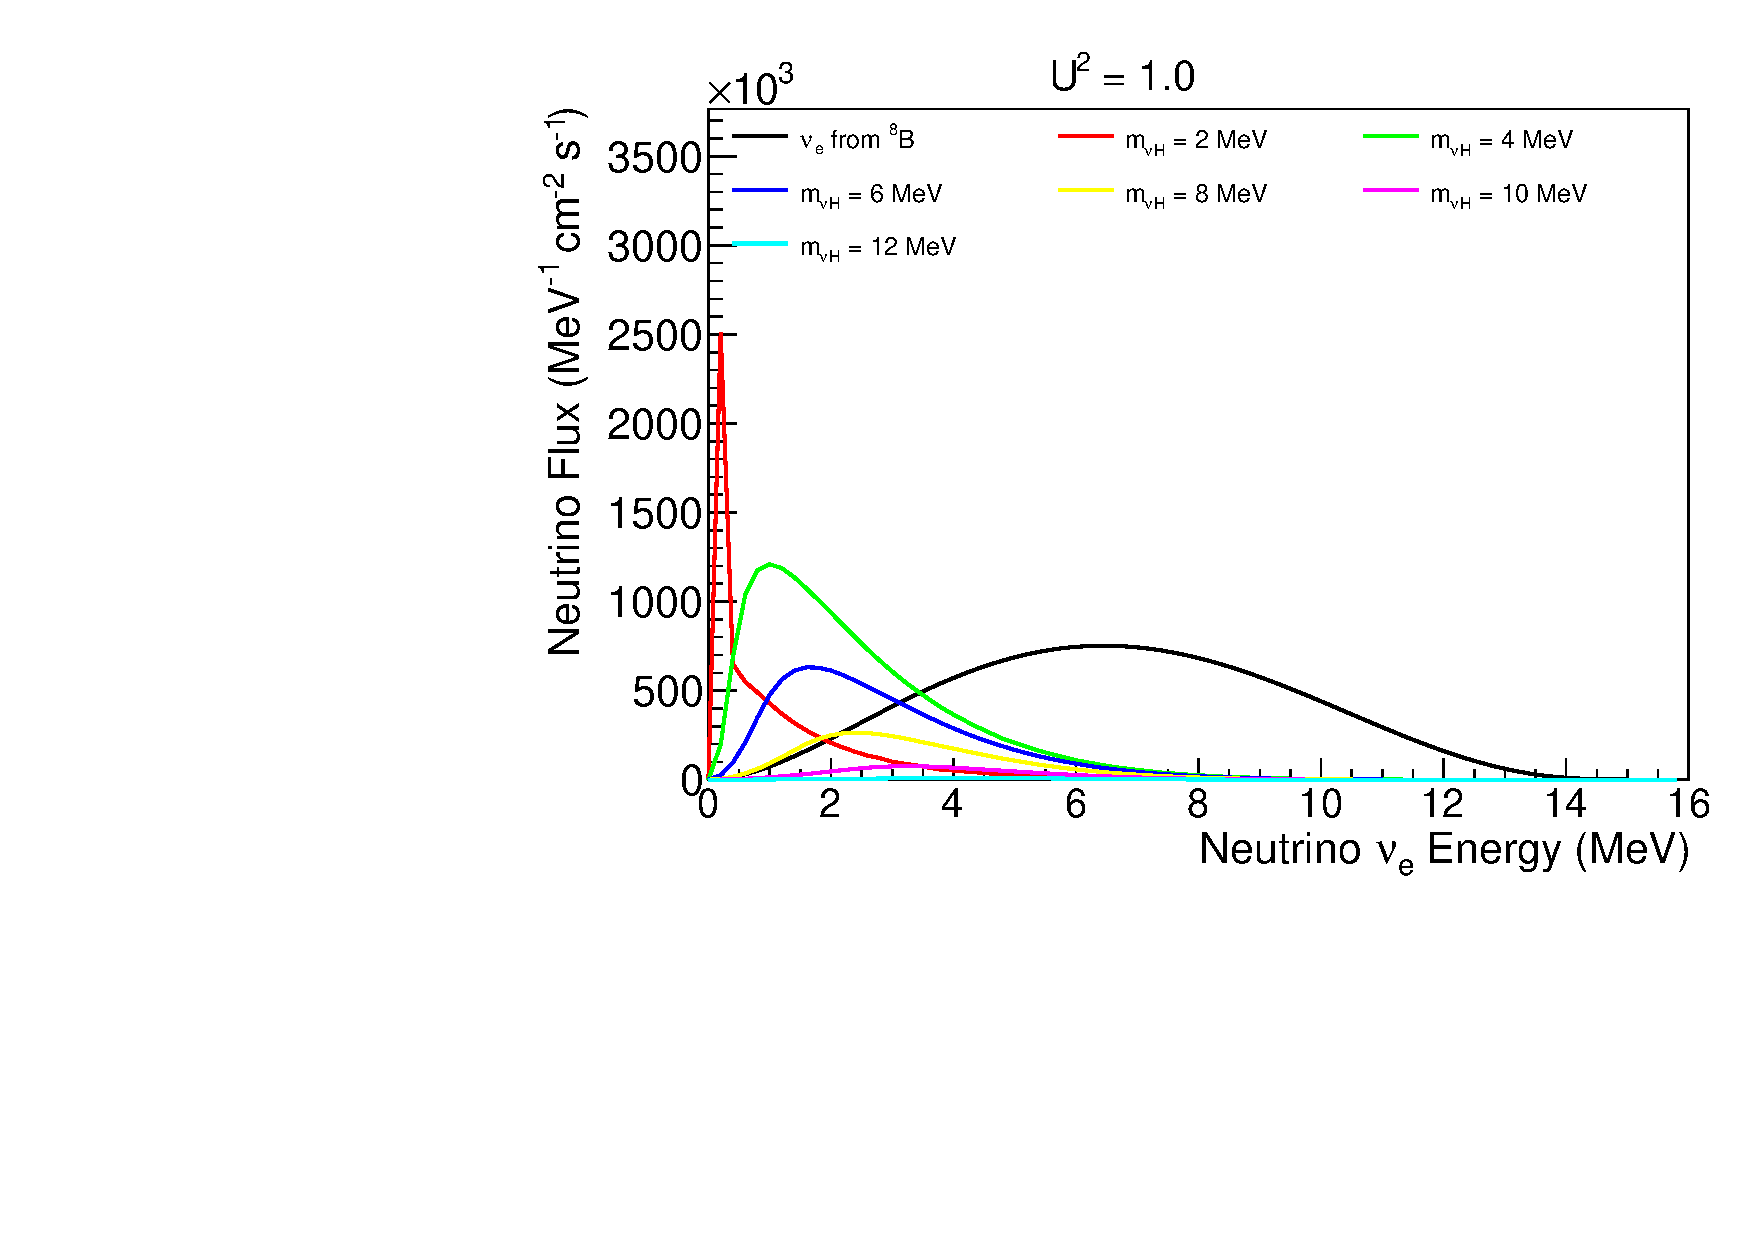
\includegraphics[width=0.99\columnwidth]{../plots/DecayInFlightNuLEnergy_U1.0_AllMass_linXlinY.pdf}
\caption{Energy spectra of $\nu_e$'s that come from $\nu_H$ decay in flight and then reach the detector on earth. Different curves are for different $\nu_H$ masses $m_{\nu H}$, and the mixing angle $|U_{eH}|^2 = 1.0$. 
The background (original solar neutrino spectrum that come from $^8 B$ decay in the Sun) spectrum is also shown in the plot.}
\label{fig:DecayInFlightSpectrum_U1em0_AllMass}
\end{figure}

\clearpage

\begin{figure}[!htbp]
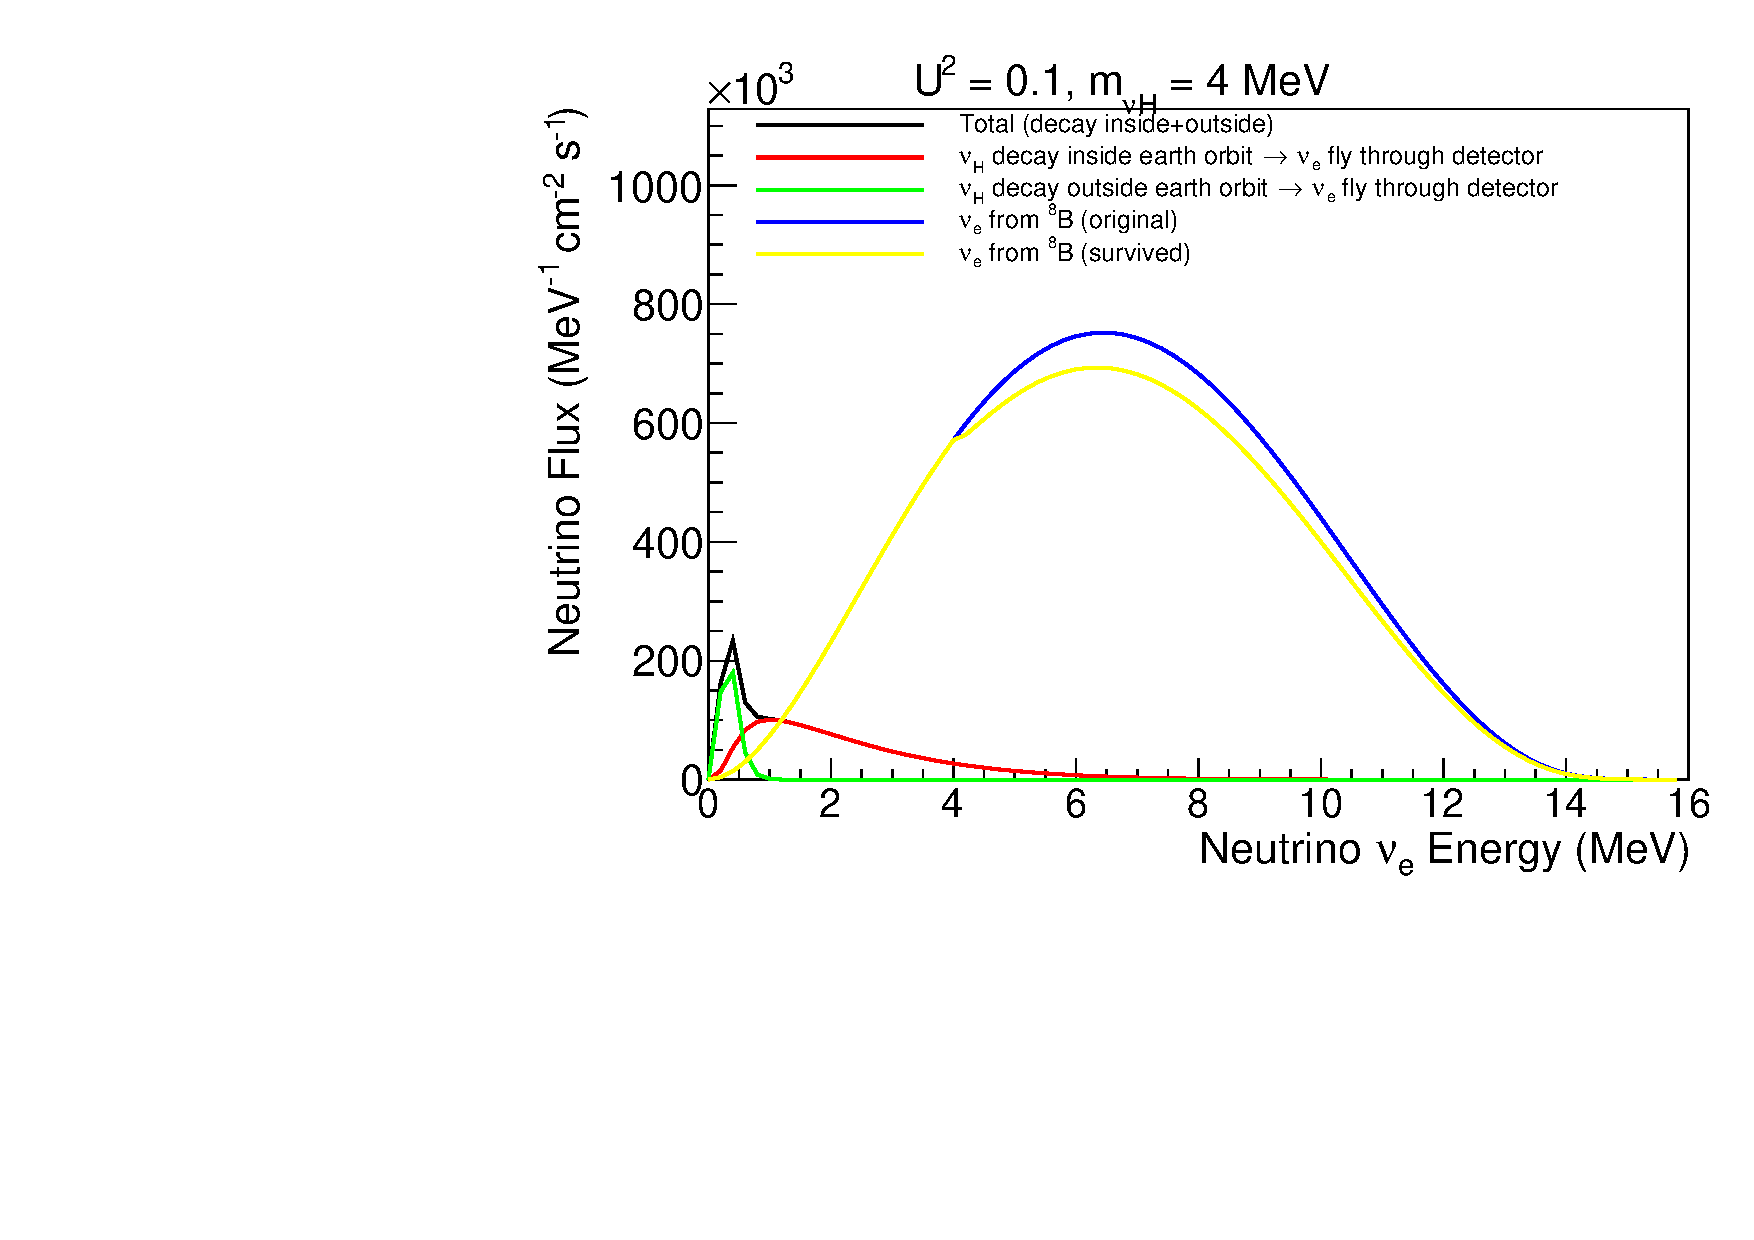
\includegraphics[width=0.99\columnwidth]{../plots/DecayInFlightNuLEnergy_U0.1_M4.0_InsideOutside_linXlinY.pdf}
\caption{Energy spectra of $\nu_e$'s that come from $\nu_H$ decay in flight and then reach the detector on earth. The spectra for $\nu_H$ decay inside and outside earth orbit are shown separately. 
The original solar neutrino spectrum that come from $^8 B$ decay in the Sun, and spectrum of solar neutrino that survived the mix to $\nu_H$ during $^{8}B$ decay, are also shown in the plot. The signal model shown in this plot is $m_{\nu H} = 4$ MeV and $|U_{eH}|^2 = 10^{-1}$.}
\label{fig:DecayInFlightSpectrum_U1em1_M4} 
\end{figure}


\begin{figure}[!htbp]
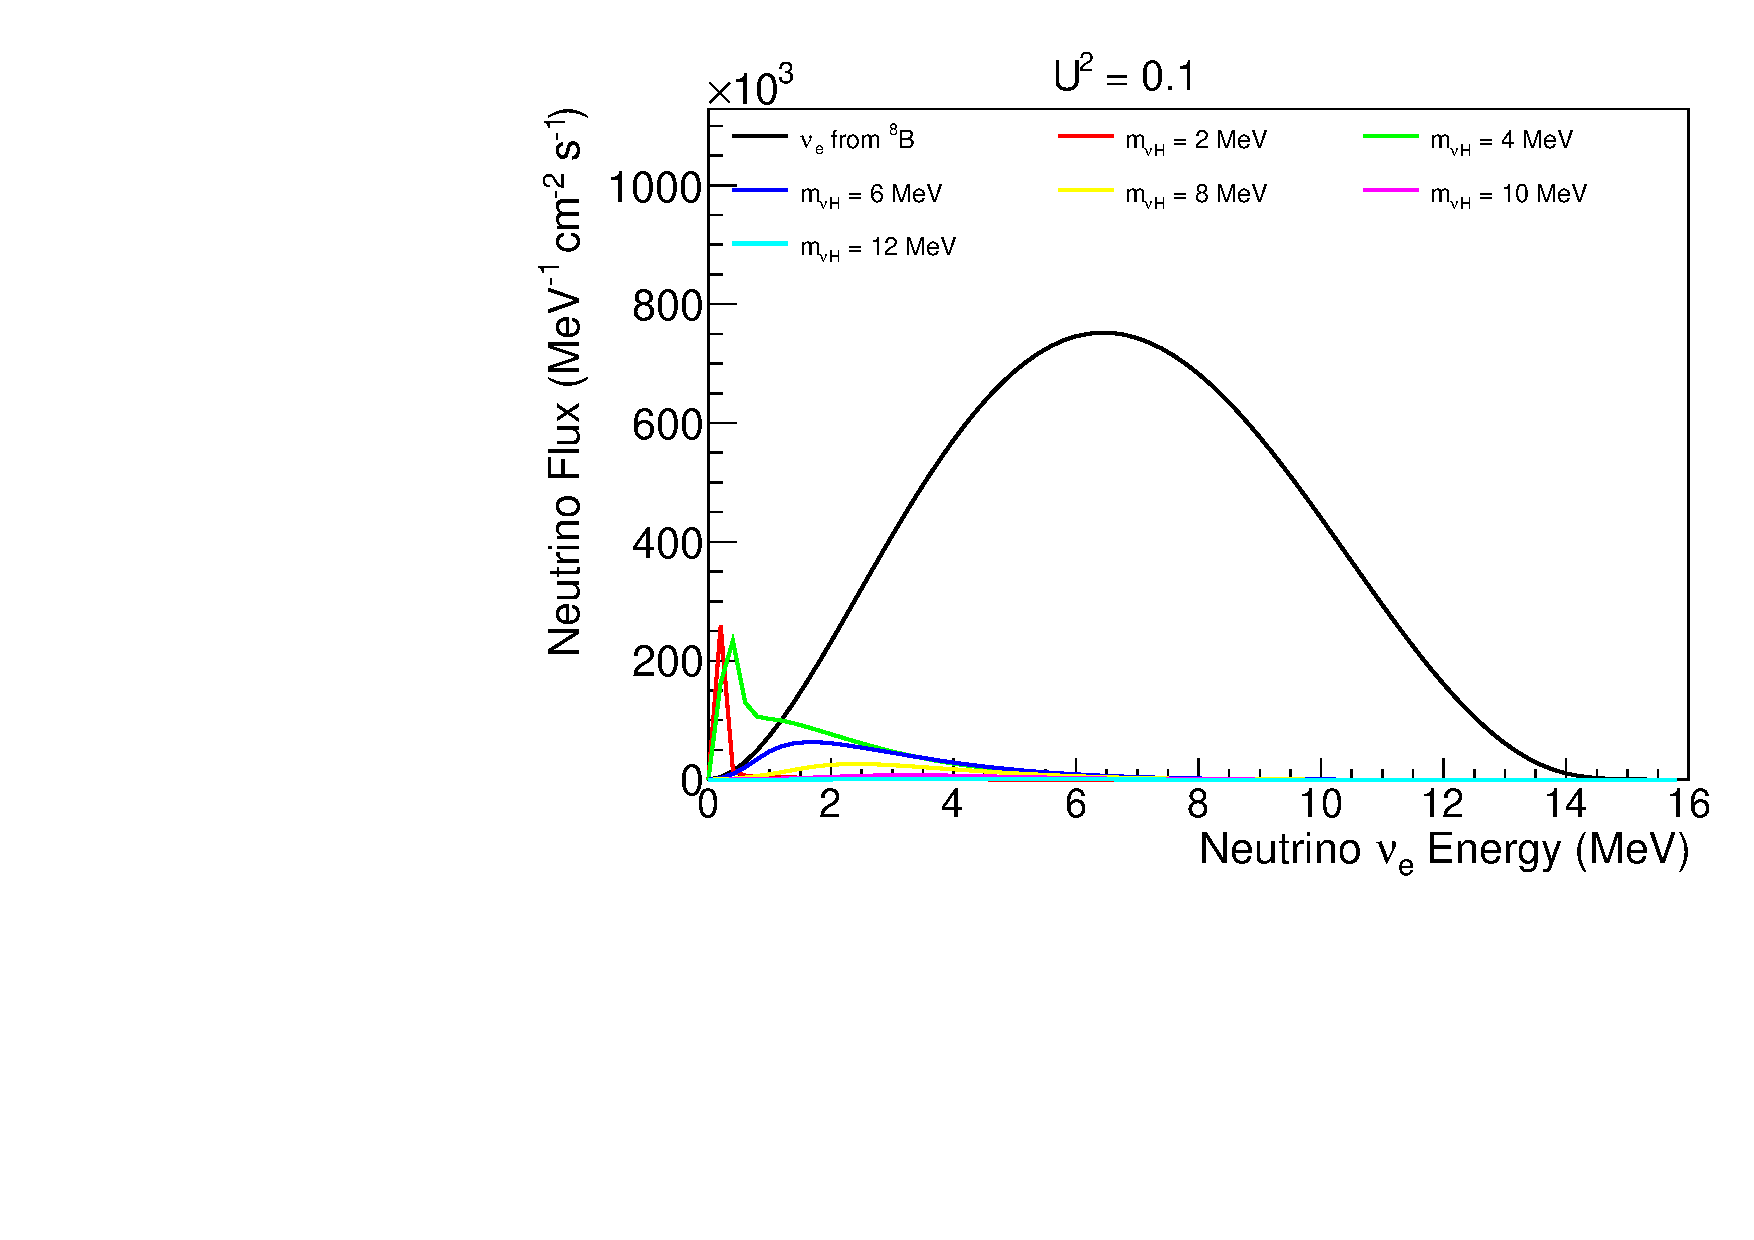
\includegraphics[width=0.99\columnwidth]{../plots/DecayInFlightNuLEnergy_U0.1_AllMass_linXlinY.pdf}
\caption{Energy spectra of $\nu_e$'s that come from $\nu_H$ decay in flight and then reach the detector on earth. Different curves are for different $\nu_H$ masses $m_{\nu H}$, and the mixing angle $|U_{eH}|^2 = 10^{-1}$. 
The background (original solar neutrino spectrum that come from $^8 B$ decay in the Sun) spectrum is also shown in the plot.}
\label{fig:DecayInFlightSpectrum_U1em1_AllMass}
\end{figure}

\begin{figure}[!htbp]
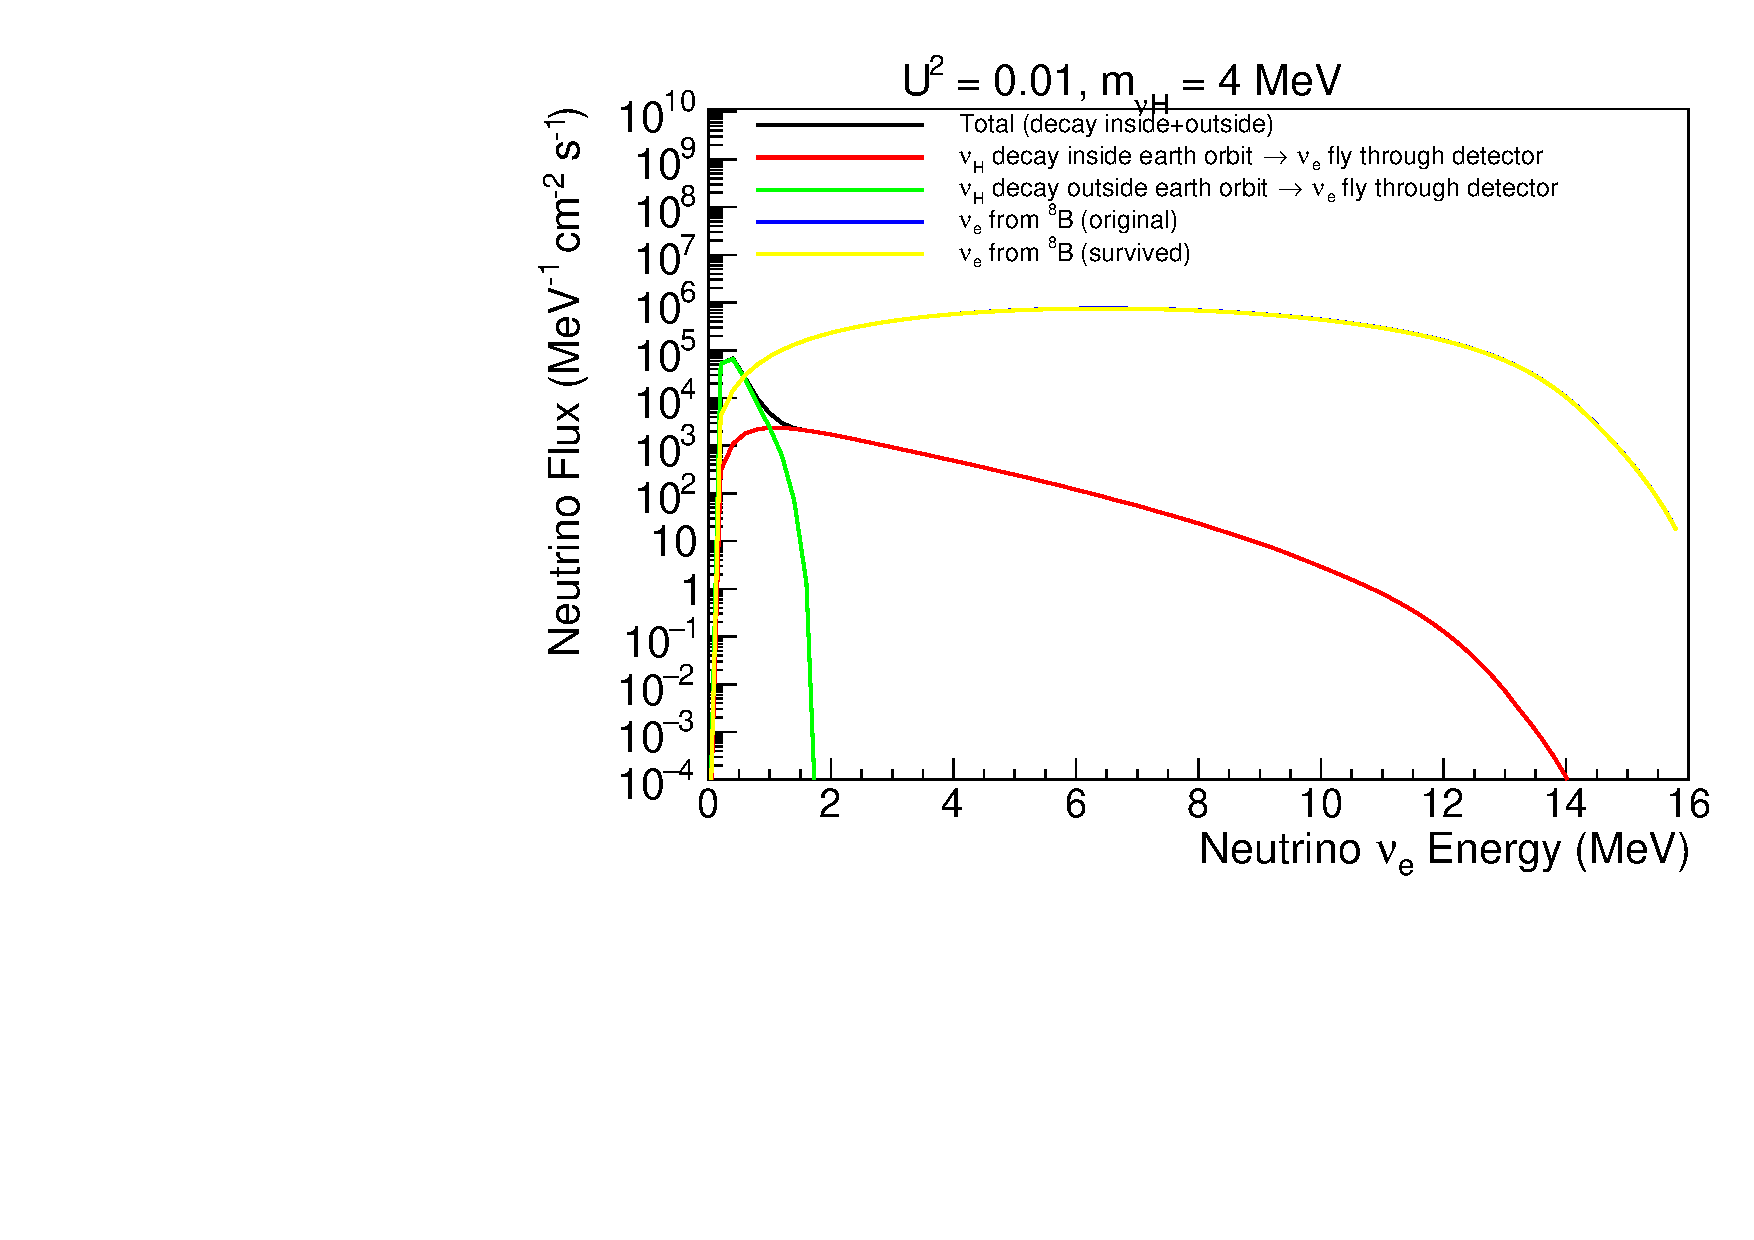
\includegraphics[width=0.99\columnwidth]{../plots/DecayInFlightNuLEnergy_U0.01_M4.0_InsideOutside_linXlogY.pdf}
\caption{Energy spectra of $\nu_e$'s that come from $\nu_H$ decay in flight and then reach the detector on earth. The spectra for $\nu_H$ decay inside and outside earth orbit are shown separately. 
The original solar neutrino spectrum that come from $^8 B$ decay in the Sun, and spectrum of solar neutrino that survived the mix to $\nu_H$ during $^{8}B$ decay, are also shown in the plot. The signal model shown in this plot is $m_{\nu H} = 4$ MeV and $|U_{eH}|^2 = 10^{-2}$.}
\label{fig:DecayInFlightSpectrum_U1em2_M4} 
\end{figure}


\begin{figure}[!htbp]
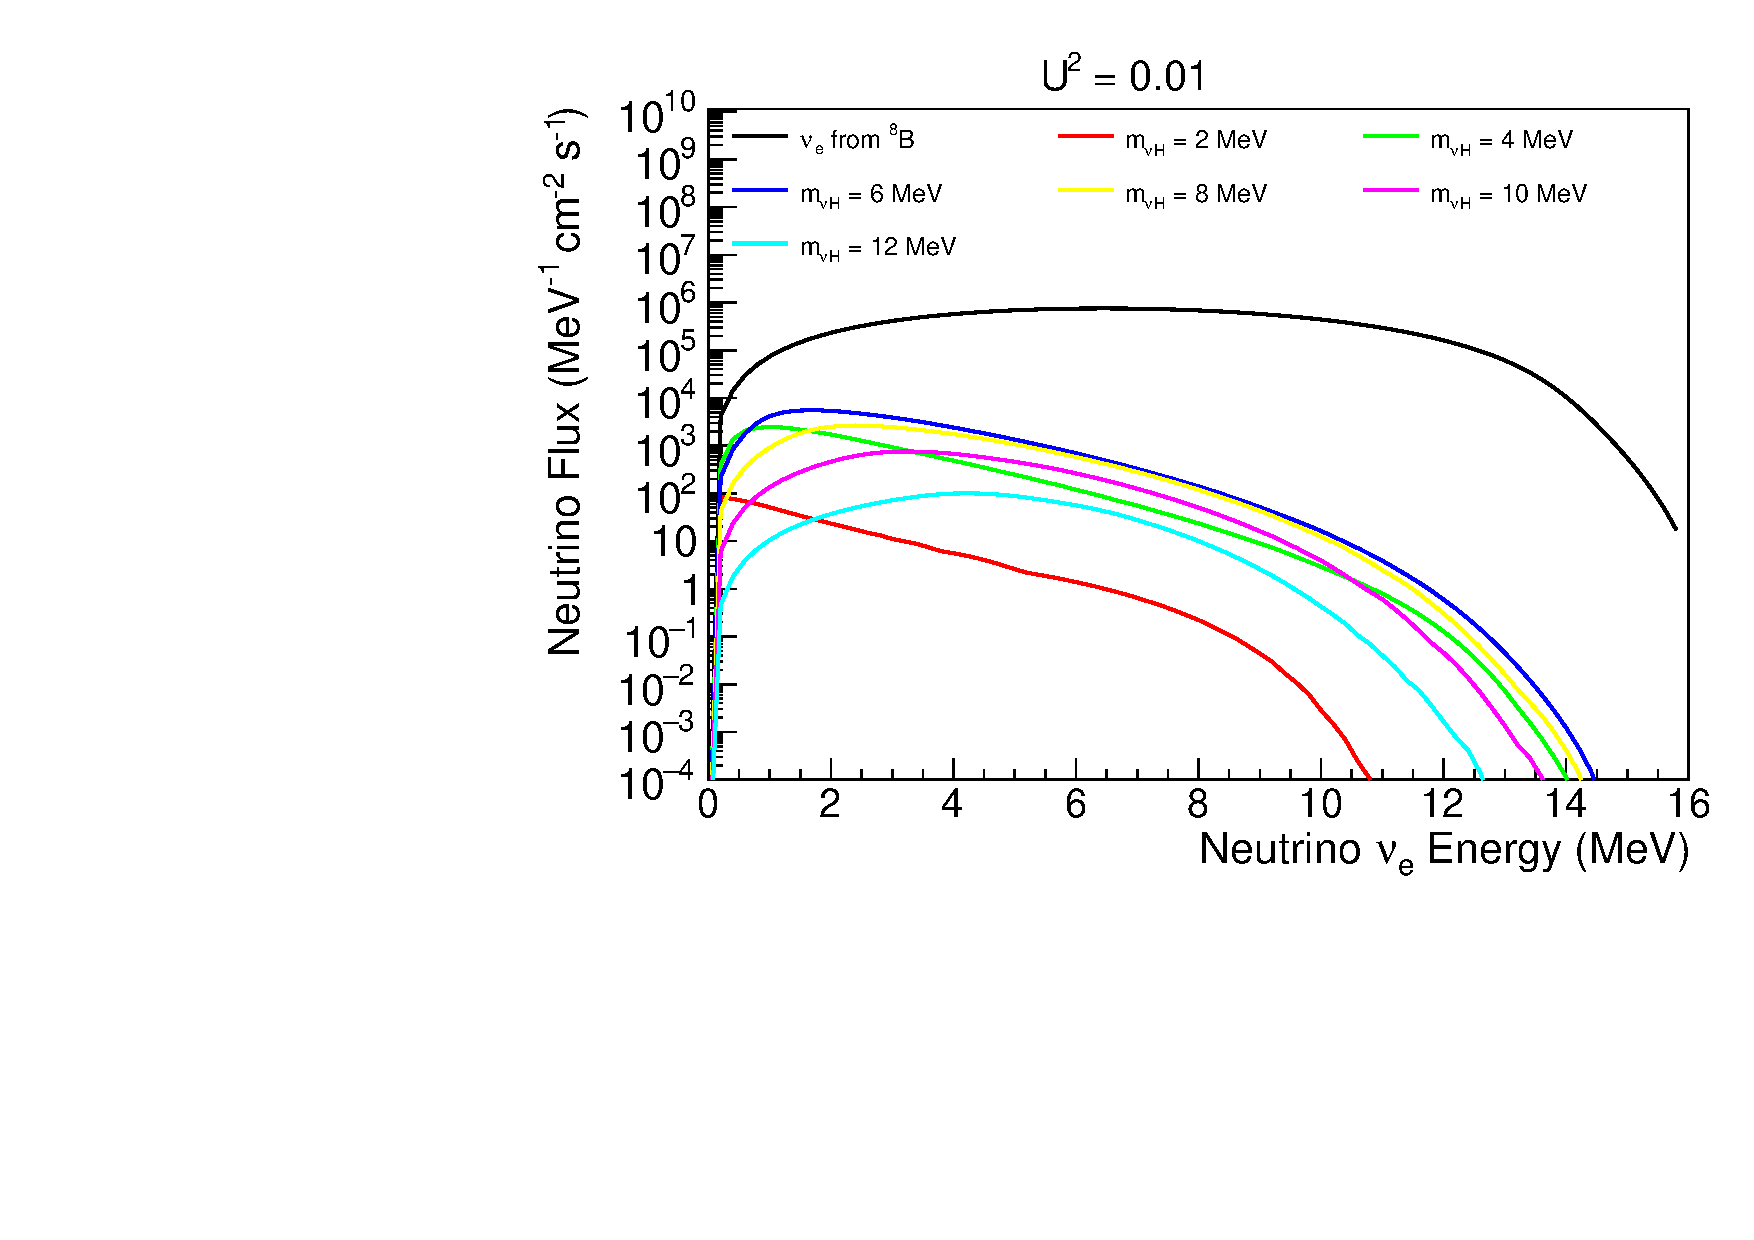
\includegraphics[width=0.99\columnwidth]{../plots/DecayInFlightNuLEnergy_U0.01_AllMass_linXlogY.pdf}
\caption{Energy spectra of $\nu_e$'s that come from $\nu_H$ decay in flight and then reach the detector on earth. Different curves are for different $\nu_H$ masses $m_{\nu H}$, and the mixing angle $|U_{eH}|^2 = 10^{-2}$. 
The background (original solar neutrino spectrum that come from $^8 B$ decay in the Sun) spectrum is also shown in the plot.}
\label{fig:DecayInFlightSpectrum_U1em2_AllMass}
\end{figure}

\begin{figure}[!htbp]
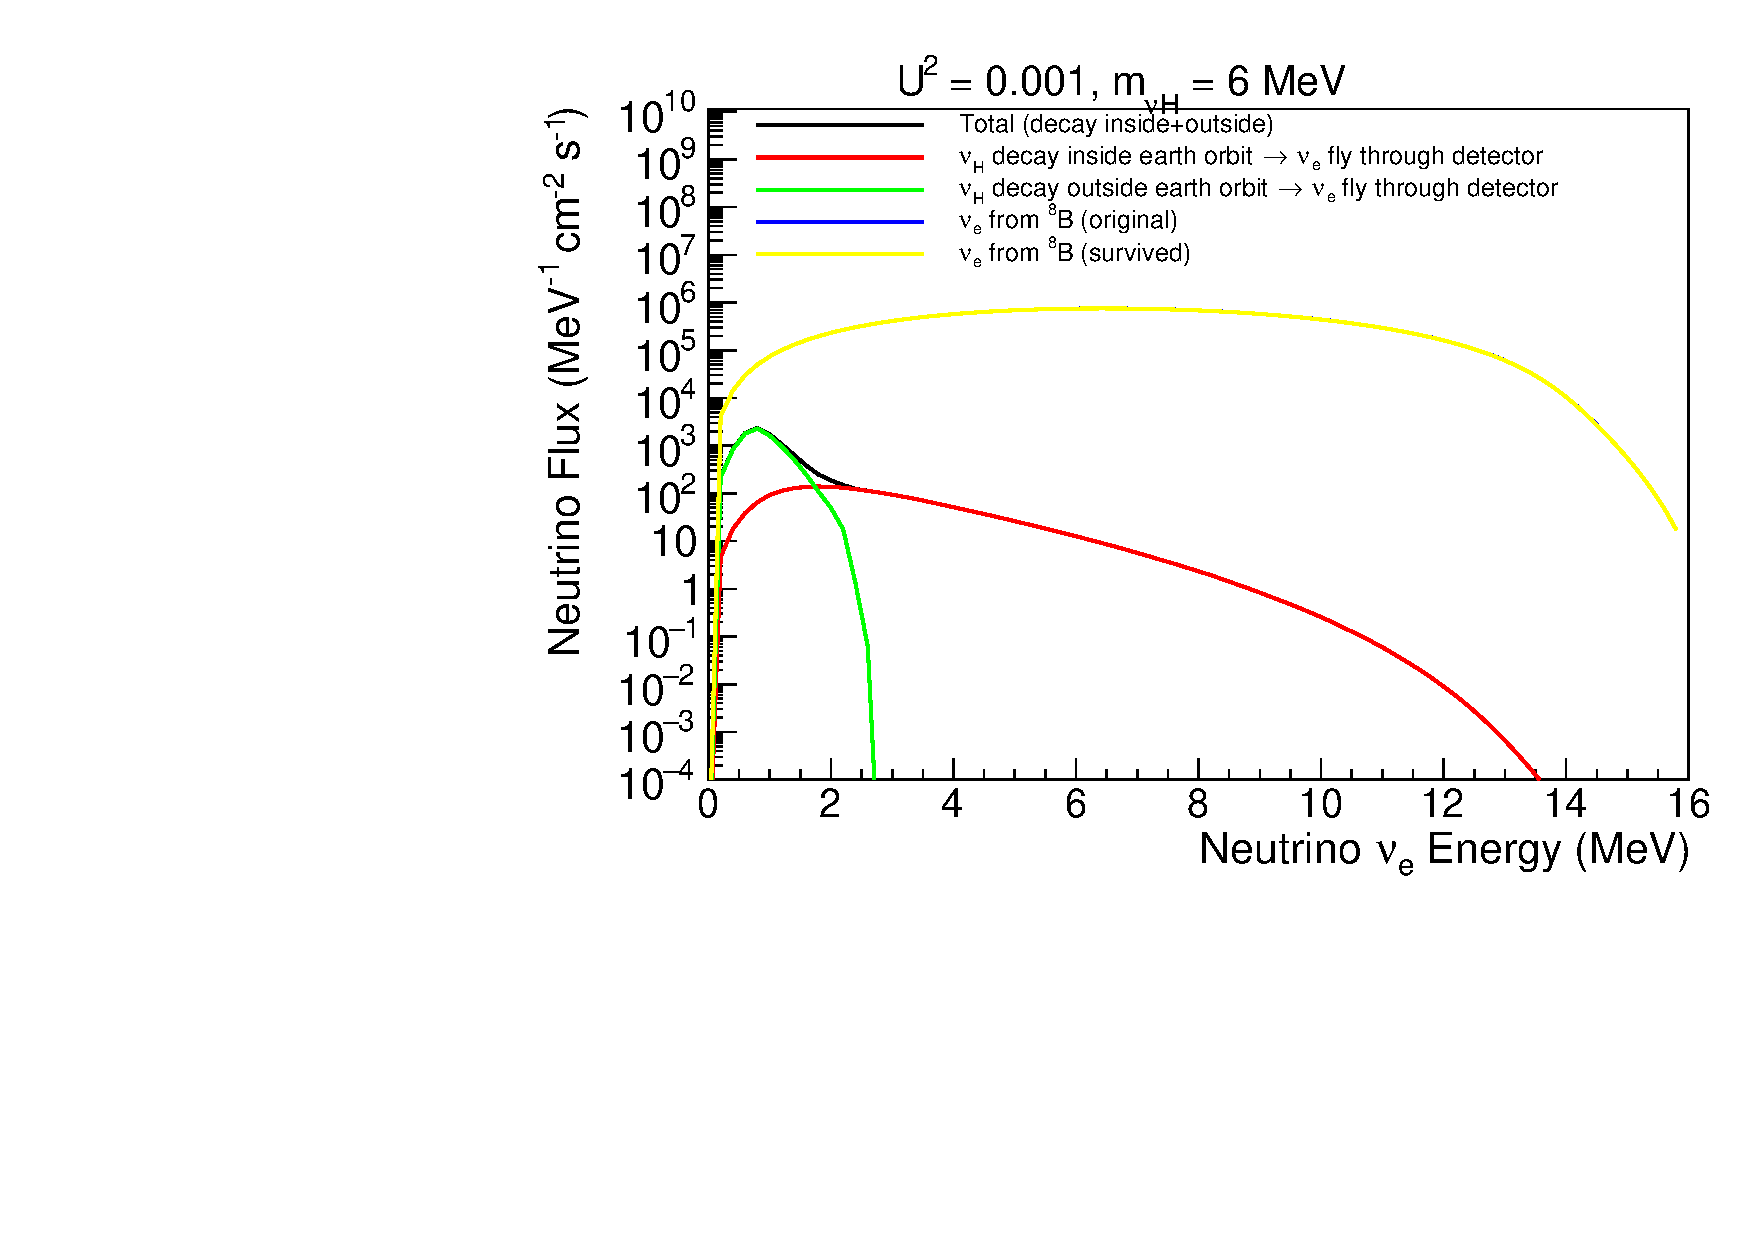
\includegraphics[width=0.99\columnwidth]{../plots/DecayInFlightNuLEnergy_U0.001_M6.0_InsideOutside_linXlogY.pdf}
\caption{Energy spectra of $\nu_e$'s that come from $\nu_H$ decay in flight and then reach the detector on earth. The spectra for $\nu_H$ decay inside and outside earth orbit are shown separately. 
The original solar neutrino spectrum that come from $^8 B$ decay in the Sun, and spectrum of solar neutrino that survived the mix to $\nu_H$ during $^{8}B$ decay, are also shown in the plot. The signal model shown in this plot is $m_{\nu H} = 6$ MeV and $|U_{eH}|^2 = 10^{-3}$.}
\label{fig:DecayInFlightSpectrum_U1em3_M6} 
\end{figure}


\begin{figure}[!htbp]
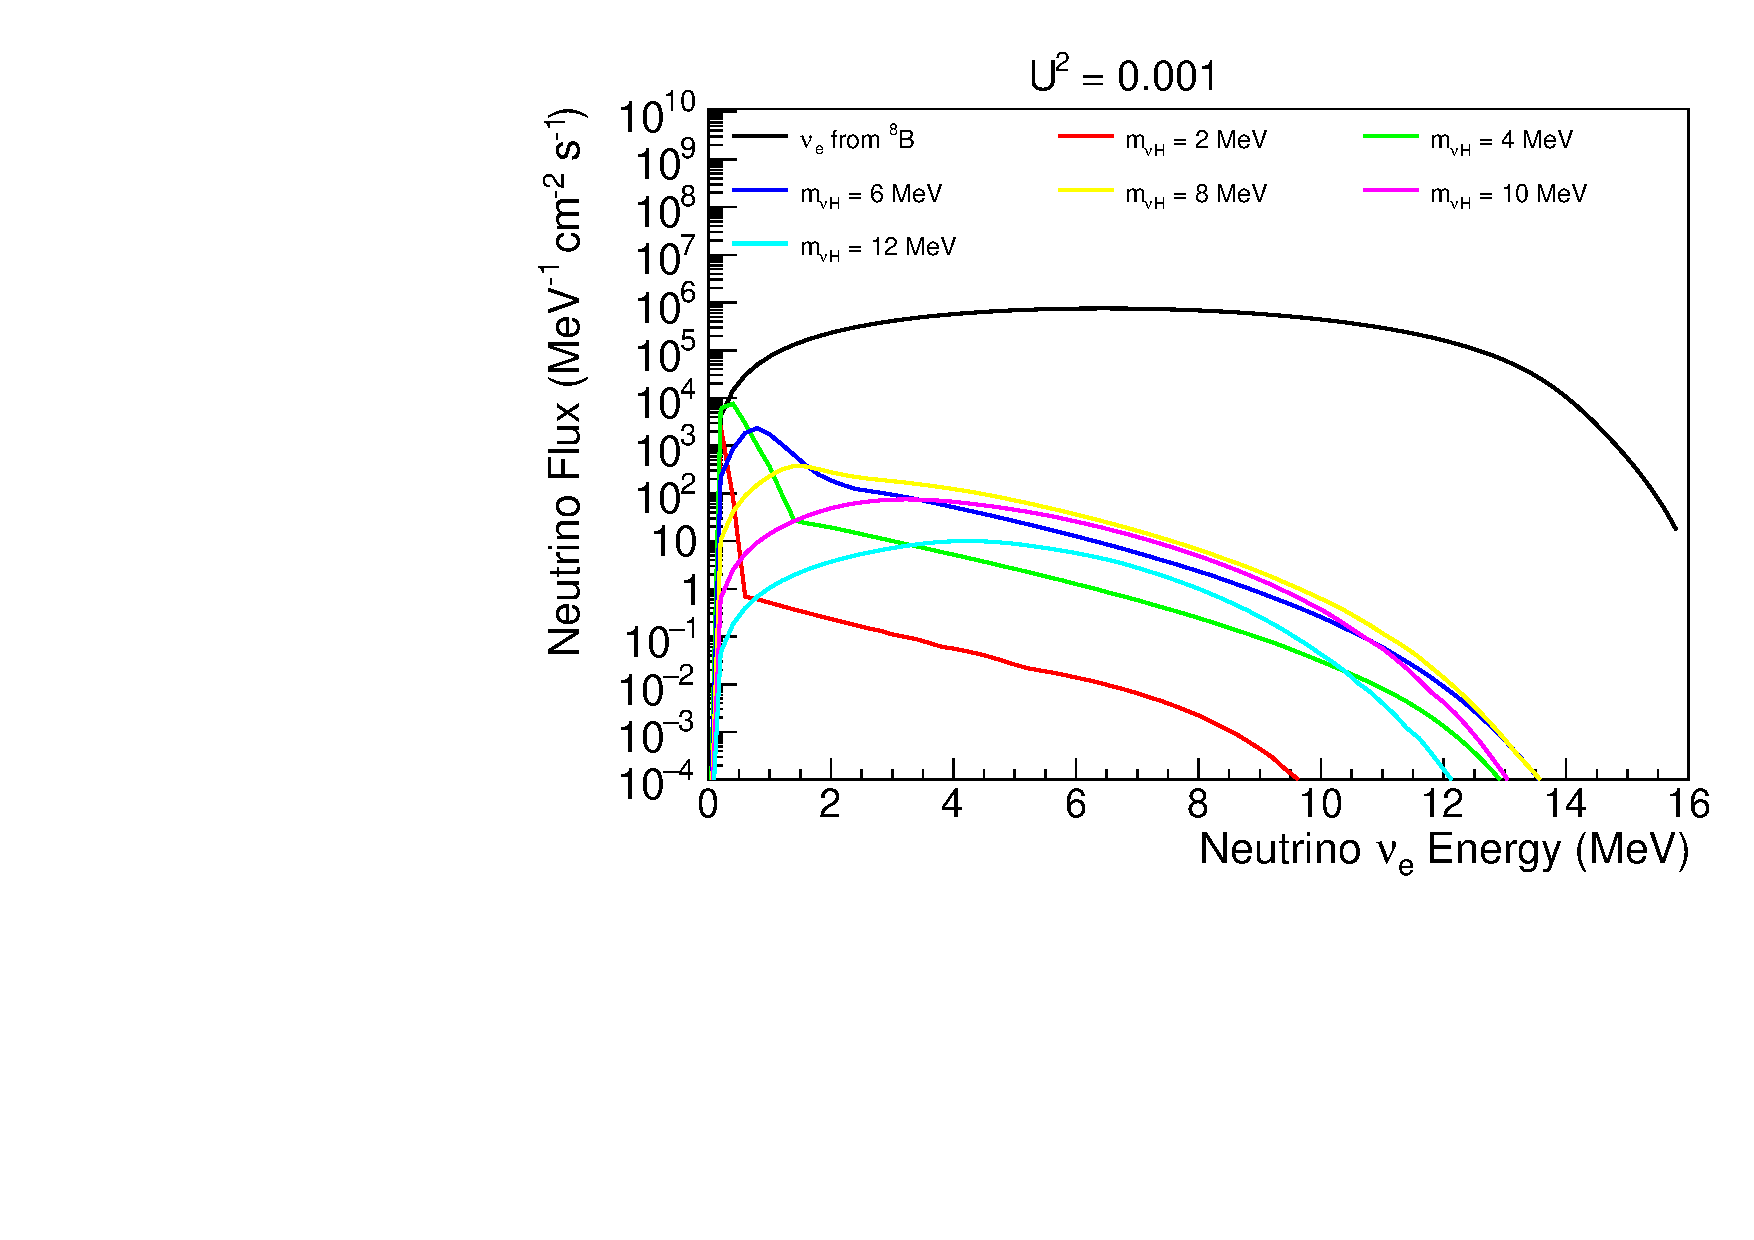
\includegraphics[width=0.99\columnwidth]{../plots/DecayInFlightNuLEnergy_U0.001_AllMass_linXlogY.pdf}
\caption{Energy spectra of $\nu_e$'s that come from $\nu_H$ decay in flight and then reach the detector on earth. Different curves are for different $\nu_H$ masses $m_{\nu H}$, and the mixing angle $|U_{eH}|^2 = 10^{-3}$. 
The background (original solar neutrino spectrum that come from $^8 B$ decay in the Sun) spectrum is also shown in the plot.}
\label{fig:DecayInFlightSpectrum_U1em3_AllMass}
\end{figure}


\begin{figure}[!htbp]
\includegraphics[width=0.99\columnwidth]{../plots/DecayInFlightNuLEnergy_U0.0001_M8.0_InsideOutside_linXlogY.pdf}
\caption{Energy spectra of $\nu_e$'s that come from $\nu_H$ decay in flight and then reach the detector on earth. The spectra for $\nu_H$ decay inside and outside earth orbit are shown separately. 
The original solar neutrino spectrum that come from $^8 B$ decay in the Sun, and spectrum of solar neutrino that survived the mix to $\nu_H$ during $^{8}B$ decay, are also shown in the plot. The signal model shown in this plot is $m_{\nu H} = 8$ MeV and $|U_{eH}|^2 = 10^{-4}$.}
\label{fig:DecayInFlightSpectrum_U1em4_M8} 
\end{figure}


\begin{figure}[!htbp]
\includegraphics[width=0.99\columnwidth]{../plots/DecayInFlightNuLEnergy_U0.0001_AllMass_linXlogY.pdf}
\caption{Energy spectra of $\nu_e$'s that come from $\nu_H$ decay in flight and then reach the detector on earth. Different curves are for different $\nu_H$ masses $m_{\nu H}$, and the mixing angle $|U_{eH}|^2 = 10^{-4}$. 
The background (original solar neutrino spectrum that come from $^8 B$ decay in the Sun) spectrum is also shown in the plot.}
\label{fig:DecayInFlightSpectrum_U1em4_AllMass}
\end{figure}

\begin{figure}[!htbp]
\includegraphics[width=0.99\columnwidth]{../plots/DecayInFlightNuLEnergy_U1e-05_M8.0_InsideOutside_linXlogY.pdf}
\caption{Energy spectra of $\nu_e$'s that come from $\nu_H$ decay in flight and then reach the detector on earth. The spectra for $\nu_H$ decay inside and outside earth orbit are shown separately. 
The original solar neutrino spectrum that come from $^8 B$ decay in the Sun, and spectrum of solar neutrino that survived the mix to $\nu_H$ during $^{8}B$ decay, are also shown in the plot. The signal model shown in this plot is $m_{\nu H} = 8$ MeV and $|U_{eH}|^2 = 10^{-5}$.}
\label{fig:DecayInFlightSpectrum_U1em5_M8} 
\end{figure}


\begin{figure}[!htbp]
\includegraphics[width=0.99\columnwidth]{../plots/DecayInFlightNuLEnergy_U1e-05_AllMass_linXlogY.pdf}
\caption{Energy spectra of $\nu_e$'s that come from $\nu_H$ decay in flight and then reach the detector on earth. Different curves are for different $\nu_H$ masses $m_{\nu H}$, and the mixing angle $|U_{eH}|^2 = 10^{-5}$. 
The background (original solar neutrino spectrum that come from $^8 B$ decay in the Sun) spectrum is also shown in the plot.}
\label{fig:DecayInFlightSpectrum_U1em5_AllMass}
\end{figure}




%\section{\label{sec:summary} Summary }

\clearpage

\bibliography{reference}

\end{document}
